\documentclass{article}
\usepackage[utf8]{inputenc}
\usepackage[main=russian,english]{babel}
\usepackage{geometry}
\usepackage{tabularx}
\usepackage[fontsize=12pt]{scrextend}
\geometry{a4paper, top=2cm}
\usepackage[colorlinks,linkcolor=black, urlcolor=cyan, citecolor=blue]{hyperref} %гиперссылки
\usepackage{graphicx}
\usepackage{xcolor}
\DeclareGraphicsExtensions{.jpg, .png}
\usepackage{float} %для H в figure
\usepackage{enumitem} %настрока перечислений

\usepackage[bottom]{footmisc} % фиксируем сноски внизу страницы

\usepackage{listings}

\usepackage[pagesize]{typearea} 

\usepackage{stringenc}
\usepackage{amsmath} 

\usepackage{caption}
\captionsetup[lstlisting]{justification=centering}

\lstset{
    language=C++,
    basicstyle=\ttfamily\normalsize,
    frame=single,
    numbers=left,
    captionpos=b,
    breaklines=true,
    extendedchars=false,
    keywordstyle=\color{black},
    commentstyle=\color{black},
    stringstyle=\color{black},
    keepspaces=true,           
    columns=flexible
}

\newcolumntype{L}{>{\raggedright\arraybackslash}X}

\begin{document}

%ТИтульник
\thispagestyle{empty}
\begin{center}
{\large 
МИНОБРНАУКИ РОССИЙСКОЙ ФЕДЕРАЦИИ \\ФЕДЕРАЛЬНОЕ ГОСУДАРСТВЕННОЕ  
АВТОНОМНОЕ ОБРАЗОВАТЕЛЬНОЕ УЧРЕЖДЕНИЕ \\ ВЫСШЕГО ОБРАЗОВАНИЯ \\ \vspace{7pt} \textbf{«САНКТ-ПЕТЕРБУРГСКИЙ ПОЛИТЕХНИЧЕСКИЙ УНИВЕРСИТЕТ ПЕТРА ВЕЛИКОГО»}\\ \vspace{7pt} Институт компьютерных наук и кибербезопасности\\ \vspace{4pt} Высшая школа технологий искусственного ителлекта\\ \vspace{4pt} Направление: 02.03.01 «Математика и компьютерные науки»

\vspace{100pt}
\textbf{Отчет о выполнении курсовой роботы}\\ \textbf{по дисциплине «Теоретические основы баз данных»}
\\ \vspace{5pt} \textbf{ на тему: «Организация выставочной деятельности музея» }
}
\end{center}

\vspace{70pt}
\noindent Выполнил студент группы 5130201/40002 \vspace{-25pt} \begin{flushright} \underline{\hspace{4cm}} Гасов А.Е. \hspace{0pt}
\end{flushright} \par

\noindent Принял доцент к.т.н.\vspace{-25pt}\begin{flushright} \underline{\hspace{4cm}} Попов С.Г. \end{flushright}

\vspace{70pt}
\begin{flushright}
    «\underline{\hspace{0.6cm}}» \underline{\hspace{2.5cm}} 2026 г.
\end{flushright}

\vspace{60pt}
\begin{center}
Санкт-Петербург \\ 2026
\end{center}

\newpage

%Содержание
\tableofcontents
\newpage

%Введение
\noindent
{\Large \textbf{\section*{Реферат}}}\par
\addcontentsline{toc}{section}{Реферат} \par

Курсовая работа посвящена предметной области <<Организация выставочной деятельности музея>>. 
Основной проблемой выступает отсутствие единой системы, способной каталогизировать выставки, учитывая перемещение экспонатов внутри музея, а это может привести к потере или порче экспонатов из-за неправильного экспонирования.
В рамках курсовой работы была реализована реляционна база данных, хранящая информацию о сотрудниках музея, выставках, выставочных залах музея, экспонатах и особенностях их хранения и экспонирования.
Для реализации базы данных была использована СУБД PostgreSQL, язык программирования Python и язык управления реляционными БД SQL.
Программу можно использовать для организации выставочной деятельности исторических музеев и музеев изобразительных искусств.

\newpage

\noindent
\vspace{-60pt}

{\Large \textbf{\section*{Введение}}}\par
\addcontentsline{toc}{section}{Введение} \par

Основной проблемой рассматриваемой предметной области «Организация выставочной деятельности музея» выступает отсутствие единой системы, способной осуществлять каталогизацию и контроль перемещения экспонатов внутри музея.
При регулярной организации новых выставок, из-за отсутствия четкого контроля перемещения экспонатов, не исключены потери экспонатов при перевозке из залов в фондохранилища и обратно.

Другая проблема — это сохранность экспонатов. Каждому экспонату нужны свои условия: определенная температура, влажность, свет или специальная витрина. Если поставить старинную картину или вещь в зал, который для этого не предназначен, она может испортиться или вовсе разрушиться. Поэтому важно, чтобы система сама проверяла, подходят ли условия зала для конкретного экспоната.

Для решения указанных проблем была спроектирована и реализована реляционная база данных, хранящая информацию о сотрудниках музея, планируемых и текущих выставках, характеристиках выставочных залов, а также о самих экспонатах и особенностях их хранения и экспонирования.

Для реализации БД была выбрана система управления базами данных PostgreSQL. Данный выбор обусловлен поддержкой возможности масштабирования под большие объёмы данных. Взаимодействие с БД осуществлялось при помощи языка SQL. Логика управления создания и заполнения таблиц была реализована на языке программирования Python, потому что он предоставляет множество библиотек для обработки и визуализации данных, например Mathplotlob.

\newpage

%Постановка задачи
%\noindent
{\Large \textbf{\section{Постановка задачи}}}\par
Цель работы: реализовать калькулятор «большой» конечной арифметики $<Z_{11}^8;+,*>$ для варианта D2, который задан правилом «+1»: \par 

\vspace{8pt}

\begin{center}
    \begin{tabular}{|c|c|c|c|c|c|c|c|c|c|c|c|c|}
    \hline
    \multicolumn{2}{|c|}{Вариант} & \multicolumn{11}{c|}{Правило «+1»} \\
    \hline
    № & $Z_i$ & a & b & c & d & e & f & g & h & i & j & k \\
    \hline
    D2 & $Z_{11}$ & b & d & a & f & c & i & j & e & k & h & g \\
    \hline
    \end{tabular}
\end{center}

\vspace{8pt}

\noindent и выполняются свойства коммутативности $(+,*)$, ассоциативности $(+, *)$,
дистрибутивности * относительно +, заданы аддитивная единица «a» и
мультипликативная единица «b», а также выполняется свойство: для ($\forall$х) х*a=a.

\vspace{10pt}
Для достижения этой цели необходимо решить задачи:
%\vspace{7pt}
\begin{enumerate}[itemsep=-3pt]
    \item Создать сложение в «малой» конечной арифметике в соответствии с правилом +1.
    \item На основе сложения в «малой» конечной арифметике создать умножение, вычитание, деление.
    \item На основе «малой» конечной арифметики реализовать соответствующие действия для «большой» конечной арифметики.
    \item Создать методы для обработки ввода отрицательных чисел.
\end{enumerate}

\newpage

%Аналитика
\noindent
{\Large \textbf{\section{Аналитика}}} \par
\vspace{-20pt}

{\Large \textbf{\subsection{Описание предметной области}}} \par

Предметная область охватывает организацию выставочной деятельности музея. Исторический музей - это культурно-просветительское и научно-иссле-\\довательское учреждение, которое занимается сбором, изучением, реставрацией и демонстрацией различных предметов, имеющих культурно-историческую ценность. Эта ценность определяется историками - людьми, профессионально занимающимися изучением и описанием прошлого человеческого общества, основываясь на различных материальных и нематериальных источниках. К материальным источникам можно отнести различные документы и предметы, созданные в рассматриваемые периоды истории, к нематериальным - устное народное творчество, легенды и предания. Ценность предметов может оцениваться по-разному, это зависит от временного промежутка, в который они были созданы, материалов, уникальности, религиозной и культурной значимости для определенных сообществ. \par

Фонды музея - это совокупность всех материалов, которые в соответствии с установленными правилами были приняты музеем на постоянное хранение \cite{site:sources1}. При этом, они могут храниться непосредственно в фондохранилище или находиться на экспозиции. Фондохранилище - это пространство в музее, предназначенное для хранения предметов коллекции, не находящихся на экспозиции. В этом помещении (помещениях) каждый предмет хранится в соответствии с требуемыми условиями хранения, которые включают определенный уровень влажности, температуры и освещенности. \par

За сохранность фондов отвечает хранитель фондов - это специалист, который несёт персональную ответственность за сохранность, учёт, научное описание и движение музейных предметов, закреплённых за фондами музея. Его обязанностями являются, инвентаризация, паспортизация, научное описание предметов, контроль условий хранения, контроль транспортировки предметов на выставки и реставрации, содействие работе исследователей и кураторов выставок. \par

В соответствии со значением предметов для науки и культуры, музейные фонды делятся на основной фонд и фонд научно-вспомогательных материалов. Научно-вспомогательный фонд формируется из предметов, выполняющих вспомогательную функцию, то есть научно-вспомогательных материалов. Научно-вспомогательные материалы – это предметы, помогающие в изучении других экспонатов. К ним относят экспозиционные научно-вспомогательные материалы (муляжи, копии, макеты, модели, реконструкции, планы). По своим функциям научно-вспомогательные материалы помогают представить внешний облик предмета в случае его отсутствия в музее, или в целях его сохранности (копии, муляжи), помогают уяснить строение предмета (схемы машин, механизмов), показывают связи экспонатов с историческими событиями (диаграммы, карты-схемы). Кроме того, к ним относят предметы очень плохой сохранности, которые не отвечают критериям отбора в основной фонд \cite{site:sources2}. \par

Основной фонд музея состоит из подлинных предметов. Это могут быть предметы быта и одежды, драгоценности, оружие и доспехи, карты, договоры, документы, письма, картины и гравюры, статуи, различные религиозные элементы, мебель, технические устройства, транспортные средства. Для каждого объекта хранителем фондов составляется паспорт, который заполняется данными о хронологических рамках создания, материалах, размерах, весе, принадлежности к определенной коллекции (предметам, выделенным историками в определенную группу по общности некоторых временн\'{ы}х или культурных признаков) и условиях хранения. \par

В фондах музея также работают реставраторы - специалисты, которые занимаются сохранением, консервацией и восстановлением музейных предметов. Деятельность этих работников тесно связана с хранителем фондов, потому что именно от него им поступают задачи по оценке состояния экспонатов, в том числе для последующей реставрации (процесса возвращения вещи первоначального состояния). Кроме того, реставраторы определяют условия хранения предметов в фондохранилище и передают эту информацию хранителю фондов. \par

Куратор выставок занимается разработкой новых выставок на территории музея. Выставка представляет собой организованную демонстрацию предметов из музейных фондов, объединённых общей темой и концепцией. Деятельность куратора заключается в разработке идей и концепций экспозиций, определении актуальности выбранной тематики, проектировании архитектуры выставочного пространства, реализации образовательных программ. На выставках демонстрируется ограниченная часть музейных фондов, поскольку не все экспонаты могут быть представлены публике из-за необходимости соблюдения определенных условий хранения, а иногда и потребности в реставрационных работах. \par

Всего выделяют шесть основных типов современных музейных экспозиций: созерцательный, тематический, средовой, систематический, интерактивный и прикладной. Созерцательный тип предполагает предъявление предметов преимущественно в эстетическом ключе с акцентом на эмоциональное восприятие. Тематический тип строится на включении экспонатов в более широкий исторический, социальный или культурный контекст с использованием пояснительных материалов. Средовой тип ориентирован на воссоздание атмосферы времени и пространства, в которых существовали представленные объекты. Систематический тип основывается на упорядоченном, классификационном показе собрания, нередко в формате открытого хранения с расширенной информацией. Интерактивный тип предполагает активное вовлечение посетителя в процесс познания через диалоговые и мультимедийные средства. Прикладной тип предоставляет возможность непосредственного практического взаимодействия с объектами и получения личного опыта \cite{site:sources3}. \par

Подготовка любой выставки проходит через определенную последовательность этапов. Первым идет разработка концепции. Куратор предлагает идею, учитывая научный интерес и предпочтения публики, определяет цели и задачи будущего проекта. После этого требуется отбор произведений, который происходит при работе с предметами в фондохранилище. После примерного отбора экспонатов следует согласование концепции и состава выставки с экспертами-историками и хранителем фондов. При этом необходимо, чтобы тема и концепция соответствовали стратегии выставочной работы музея на ближайшие годы. Далее следует создание заявки на выставку и составление подробной сметы расходов. После этого заявка со сметой рассматриваются директором музея. Раз в год все одобренные директором выставочные заявки отправляют в Министерство культуры, где специальная комиссия определяет, какие проекты будут поддержаны, а какие будут ждать своей очереди. \par

Если выставочный проект одобрен, то для выставки находят организатора, который занимается реализацией планов куратора.  Для этого определяется место проведения и утверждаются точные даты экспонирования, утверждается финансирование определённых закупок и услуг, необходимых для создания и проведения выставки. После согласования статей расходов начинается самый насыщенный этап - поиск исполнителей и заключение контрактов, закупка, организация транспортировки, работа над дизайном экспозиции, подготовка сопроводительных материалов, аннотаций, программы мероприятий, запуск PR-кампании выставки, освещение в СМИ и социальных сетях. Завершается подготовка монтажом выставки, который чаще всего длится 3-4 дня и включает в себя расположение экспонатов в соответствии с экспозиционным планом, оформление зала, настройку света. Этот долгий путь завершается вернисажем выставки (вернисаж - это торжественное открытие выставки, на котором присутствуют приглашенные персоны и СМИ) \cite{site:sources4}. \par


%\vspace{-10pt}
{\Large \textbf{\subsection{Цели функционирования базы данных}}} \par

\begin{enumerate}
    \item Ведение централизованного реестра музейных предметов.
    \item Ведение реестра проводимых в музее выставок.
    \item Хранение планов размещения выставок в залах музея.
\end{enumerate}


\vspace{-40pt}
{\Large \textbf{\subsection{Перечень сущностей и их атрибутов}}} \par


\begin{enumerate}
    \item \textbf{Сотрудник} - учетная запись специалиста музея, определяющая его полномочия и зону ответственности в работе с фондами или при организации выставок.
    \begin{itemize}
        \item Фамилия.
        \item Имя.
        \item Отчество.
        \item Должность (куратор, организатор, хранитель, реставратор).
        \item Номер телефона.
    \end{itemize}

    \item \textbf{Фонд} - полное собрание музейных предметов, прошедших научный отбор и принятых музеем на постоянное хранение в соответствии с установленными правилами содержания.
    \begin{itemize}
        \item Тип фонда (основной, вспомогательный).
        \item Принадлежность к коллекции (Пример: <<Ближневосточные монеты периода высокого средневековья>>).
        \item Уровень доступа.
        \item Ответственный хранитель.
    \end{itemize}

    \item \textbf{Фондохранилище} - специализированное помещение, оборудованное для долгосрочного хранения предметов коллекции, не задействованных в текущих экспозициях музея.
    \begin{itemize}
        \item Вместимость (максимальное количество объектов для размещения).
        \item Температура.
        \item Влажность.
        \item Освещенность.
    \end{itemize}

    \item \textbf{Экспонат} - предмет, который обладает культурной и научной ценностью, а также числится на хранении в фонде музея с целью изучения или участия в выставках. 
    \begin{itemize}
        \item Инвентарный номер.
        \item Название.
        \item Текущий статус (в хранилище, на экспозиции, на реставрации).
        \item Принадлежность к коллекции.
    \end{itemize}

    \item \textbf{Технический паспорт} - документ, приписанный к определенному экспонату из фондов музея, который содержит информацию о его характеристиках, состоянии и условиях содержания.
    \begin{itemize}
        \item Состояние (заключение реставратора о физической сохранности).
        \item Тип экспоната (оружие, одежда, документ, монета и др.).
        \item Вес.
        \item Эпоха.
        \item Материал.
        \item Требуемая влажность.
        \item Требуемая температура.
        \item Требуемая освещенность.
    \end{itemize}

    \item \textbf{Выставка} - временная тематическая демонстрация группы экспонатов, объединенных общей концепцией и определенными сроками показа посетителям музея.
    \begin{itemize}
        \item Название.
        \item Тема.
        \item Тип.
        \item Состояние (подбор экспонатов, согласование, организация пространства, действующая)
        \item Ответственный куратор.
    \end{itemize}

    \item \textbf{Экспозиционный план} - документ, фиксирующий перечень задействованных в выставке предметов и их размещение в выставочном пространстве.
    \begin{itemize}
        \item Версия плана (черновик, окончательная).
        \item Ответственный организатор.
        \item Необходимое количество витрин.
        \item Логика осмотра (хронологическая, тематическая, свободная).
        \item Концепция взаимодействия (атмосферная, интерактивная, традиционная выставка)
        
    \end{itemize}

    \item \textbf{Витрина} - специализированное выставочное оборудование, расположенное в залах музея и предназначенное для демонстрации экспонатов посетителям.
    \begin{itemize}
        \item Уровень освещенности.
        \item Поддерживаемая влажность.
        \item Поддерживаемая температура.
    \end{itemize}

    \item \textbf{Смета расходов} - финансовый документ, отражающий планируемые затраты на услуги логистики, страховки, монтажа, необходимые для реализации проекта выставки.
    \begin{itemize}
        \item Расходы на рекламу.
        \item Расходы на реставрацию.
        \item Расходы на создание сопровождающих материалов.
        \item Расходы на услуги наемных рабочих.
        \item Статус согласования.
    \end{itemize}

    \item \textbf{Выставочное пространство} - оборудованный зал или территория музея, предназначенная для публичного показа экспонатов, условия содержания которых подходят для данного пространства.
    \begin{itemize}
        \item Тип помещения (кабинет, арсенал, коридор).
        \item Вместимость посетителей.
        \item Уровень естественной освещенности.
        \item Уровень охраны.
    \end{itemize}
\end{enumerate}

\vspace{-40pt}
{\Large \textbf{\subsection{Перечень ролей}}} \par

\begin{enumerate}
    \item \textbf{Куратор выставок} — профессионал, разрабатывающий научную концепцию и тему выставки, а также осуществляющий подбор экспонатов из фондов музея и определяющий их роль в рамках конкретного выставочного проекта.
    \item \textbf{Организатор выставок} — специалист, отвечающий за техническую реализацию выставки, координацию логистики, закупок, монтажа экспозиции, а также ответственный за финансовый контроль утвержденной сметы расходов.
    \item \textbf{Хранитель фондов} - специалист, который несёт ответственность за сохранность, учёт, научное описание и движение музейных предметов, закреплённых за фондами музея.
    \item \textbf{Реставратор} — эксперт, занимающийся оценкой физического состояния предметов, проведением работ по их восстановлению и консервации, а также устанавливающий допустимые параметры среды для безопасного экспонирования.
\end{enumerate}

\vspace{-40pt}
{\Large \textbf{\subsection{ER-диаграмма и схема связи объектов}}} \par

ER-диаграмма с текстом ее чтения представлена на Рис.\ref{ER}. \par
Ниже выделен текст чтения ER-диаграммы.
\vspace{4pt}
\begin{enumerate}[noitemsep, topsep=0pt]
    \item Сотрудник занимает должность.
    \item Должность наделяет полномочиями.
    \item Полномочия заведовать фондом.
    \item Полномочия реставрировать экспонаты.
    \item Полномочия составлять технические паспорта.
    \item Полномочия курировать выставки.
    \item Полномочия составлять смету расходов.
    \item Фонд располагает коллекциями.
    \item Коллекция объединяет экспонаты. 
    \item Экспонат закреплен за фондохранилищем.
    \item Экспонат сопровождается техническим паспортом.
    \item Выставка реализуется по экспозиционному плану.
    \item Экспозиционный план обосновывает смету расходов.
    \item Экспозиционный план характеризует выставочное пространство.
    \item Выставочное пространство располагает местами экспонирования.
    \item Место экспонирования демонстрирует экспонат.
\end{enumerate}

\storeareas\MySavedValues 

% 2. Меняем формат на A3 и ориентацию на альбомную
% Важно: \clearpage обязателен перед сменой формата
%\clearpage
\KOMAoptions{
    paper=a3, 
    paper=landscape, 
    DIV=15,           % Делаем поля поменьше, так как на A3 их стандартный размер огромен
    BCOR=0mm,         % Убираем отступ под переплет для этого листа
    pagesize          % Гарантируем, что PDF поймет смену размера
}
\recalctypearea

\noindent
%\vspace{20pt}
\begin{figure}[H]
    \centering
    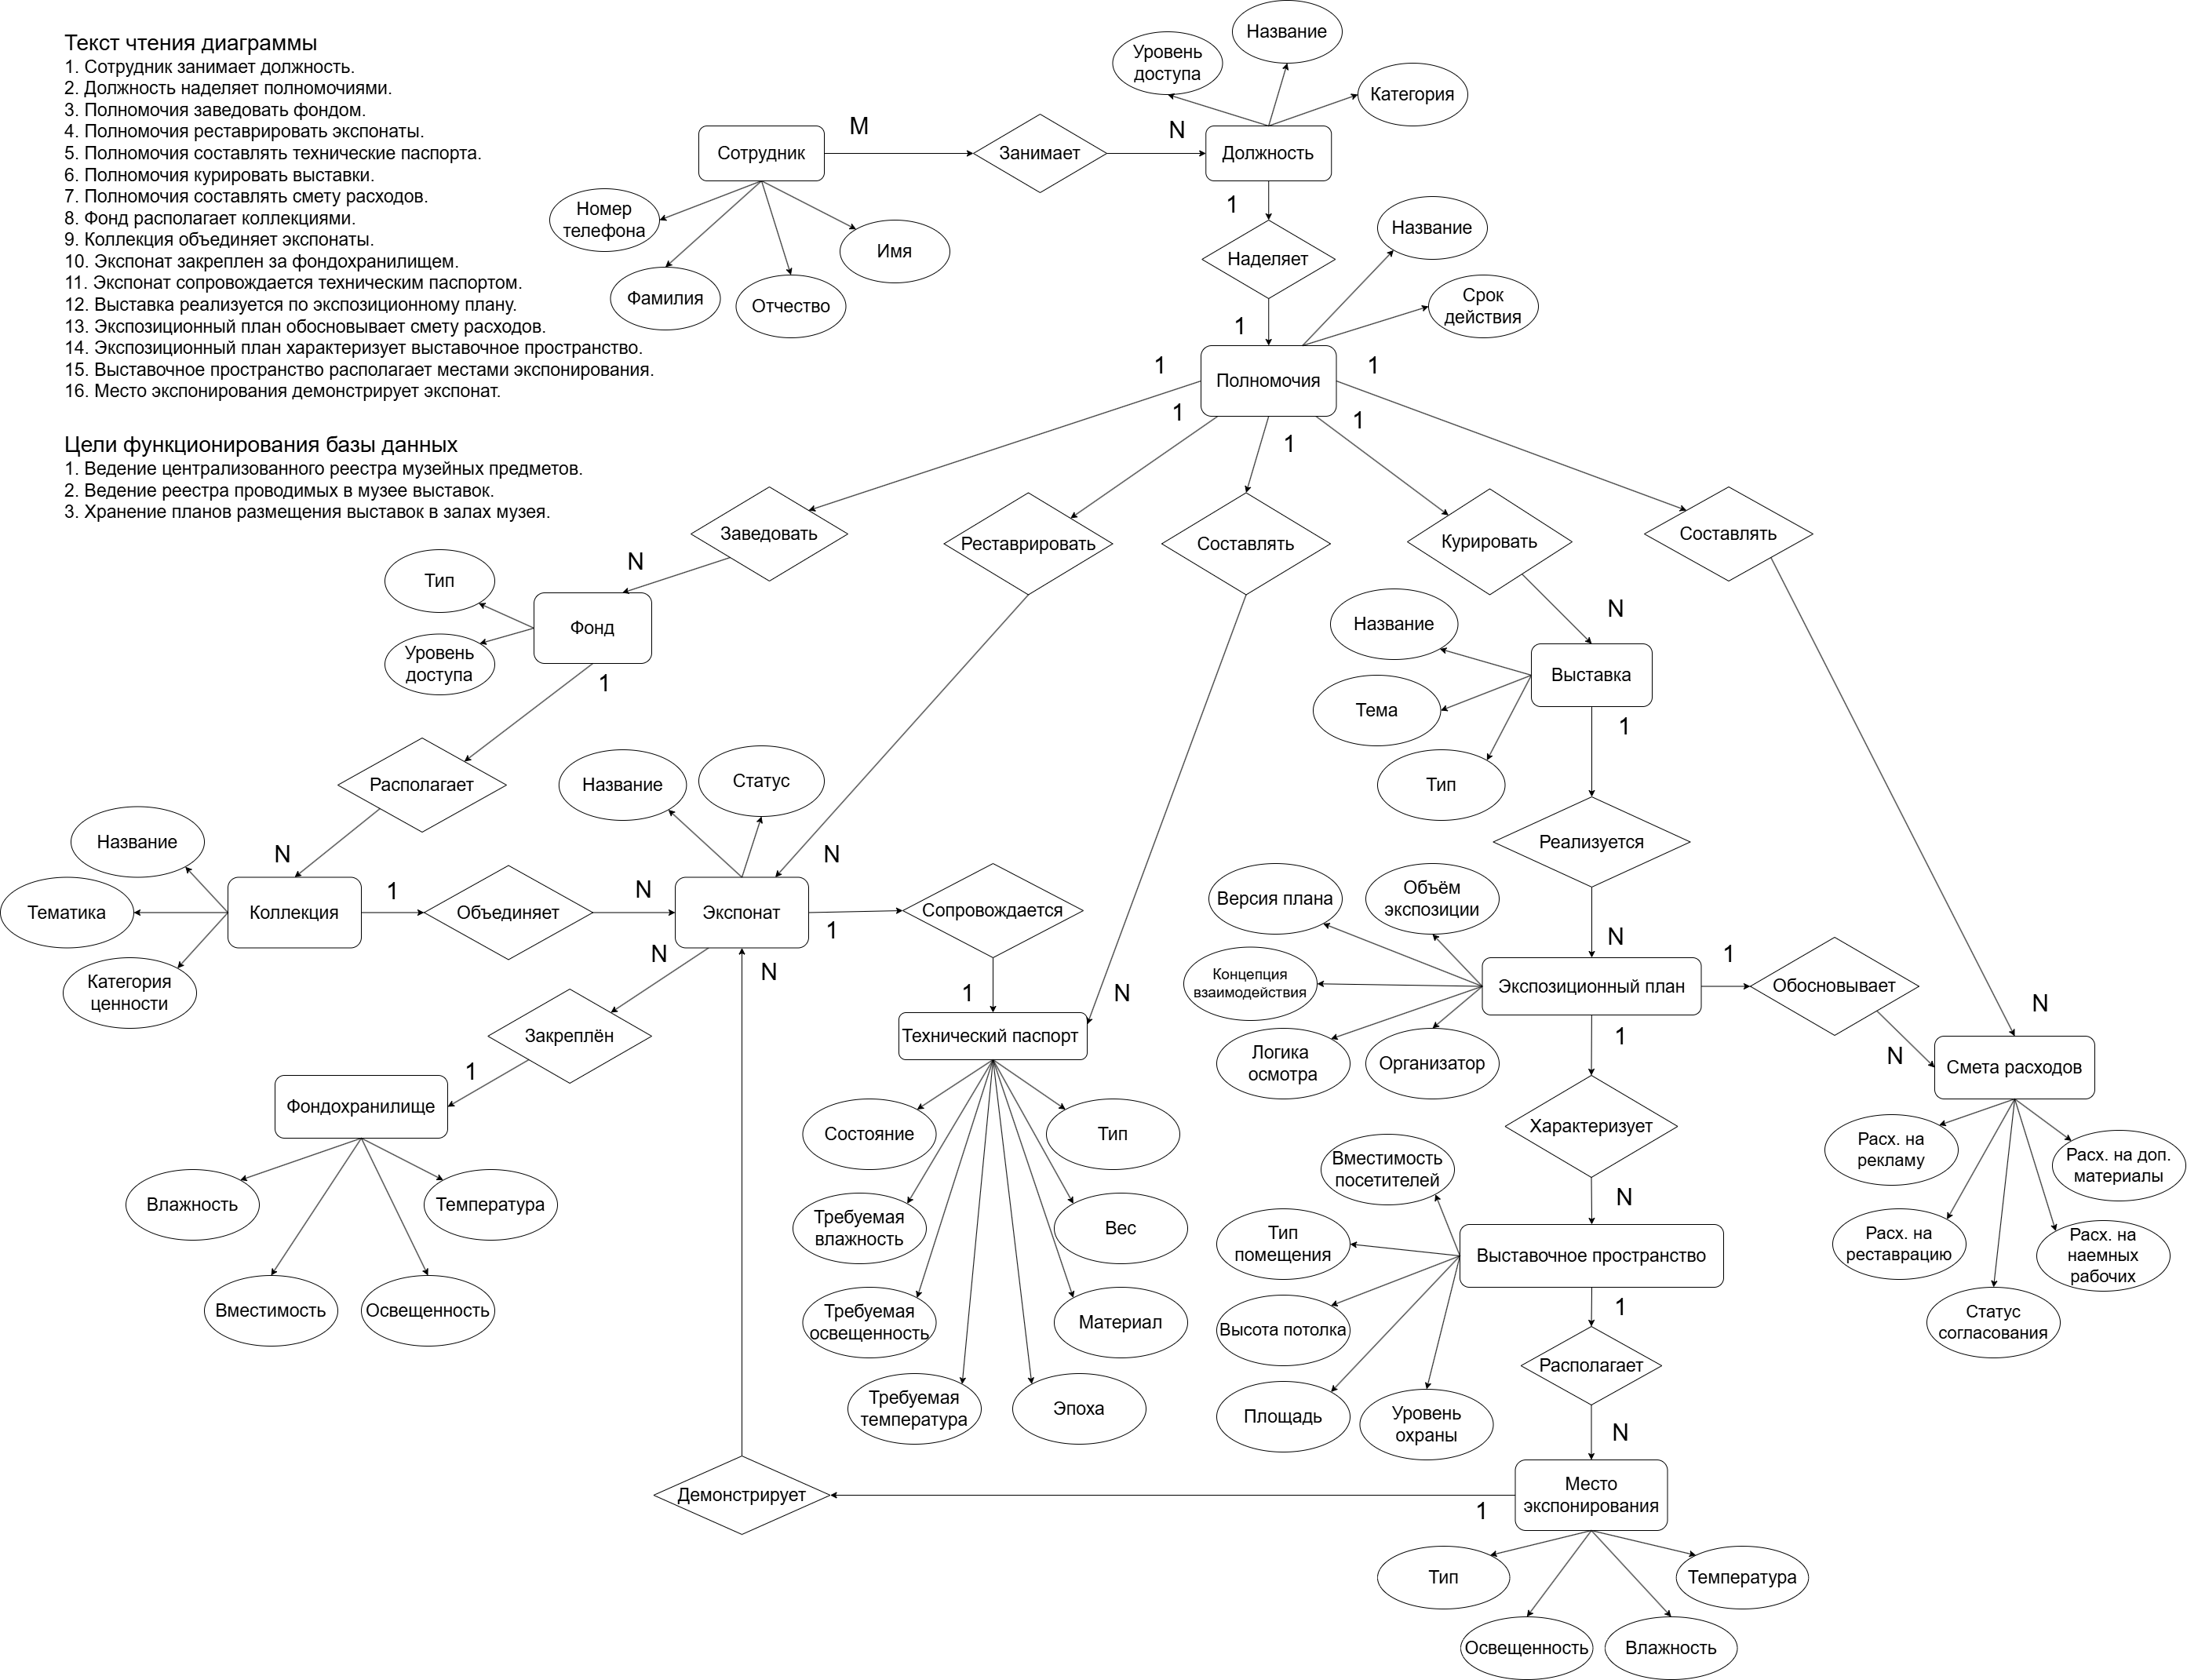
\includegraphics[height=24cm]{pic/ER версия 2.png}
    \caption{ER-диаграмма}
    \label{ER}
\end{figure}

\clearpage
\MySavedValues
\recalctypearea

\newpage


Схема связи объектов представлена на Рис.\ref{objects_shema}.

\begin{figure}[H]
    \centering
    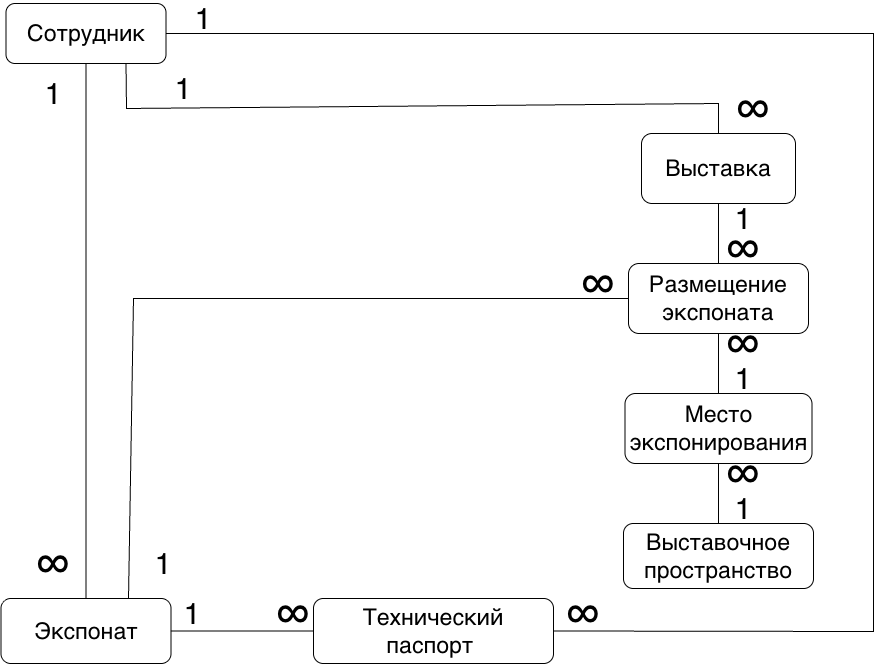
\includegraphics[height=10cm]{pic/Иерархия сокращенная.png}
    \caption{Схема связи объектов}
    \label{objects_shema}
\end{figure}


\begin{enumerate}
    \item Один сотрудник может курировать множество выставок (1 - $\infty$).
    \item За одним сотрудником может быть закреплено много экспонатов (1 - $\infty$).
    \item Один сотрудник может составить много технических паспортов (1 - $\infty$).
    \item Одно выставочное пространство включает в себя множество конкретных мест экспонирования (стендов, витрин) (1 - $\infty$).
    \item В рамках одной выставки выставляется множество экспонатов в местах экспонирования (размещение экспоната) (1 - $\infty$).
    \item Одно место экспонирования может быть связано с множеством записей о размещении экспонатов (разные предметы в разное время) (1 - $\infty$).
    \item Один экспонат может иметь разные версии технических паспортов (1 - $\infty$).
    \item Один экспонат может быть размещен в разных местах экспонирования на разных выставках (размещение экспоната) (1 - $\infty$).
\end{enumerate}

%Проектирование
\noindent
{\Large \textbf{\section{Проектирование}}} \par

% =============================================================
% СПРАВОЧНИКИ
% =============================================================
{\Large \textbf{\subsection{Лингвистическое описание схемы БД}}} \par


\begin{enumerate}
    \item exhibition\_status (exhibition\_status\_id (SERIAL), \\ exhibition\_status\_name (VARCHAR(11))).
    \item exhibition\_type (exhibition\_type\_id (SERIAL), exhibition\_type\_name \\(VARCHAR(15))).
    \item exhibition\_subject (exhibition\_subject\_id (SERIAL), exhibition\_subject\_name (VARCHAR(25))).
    \item exhibit\_status (exhibit\_status\_id (SERIAL), exhibit\_status\_name \\(VARCHAR(25))).
    \item materials (material\_id (SERIAL), material\_name (VARCHAR(25))).
    \item exhibit\_conditions (exhibit\_conditions\_id (SERIAL), exhibit\_conditions\_name (VARCHAR(18))).
    \item epochs (epoch\_id (SERIAL), epoch\_name (VARCHAR(30))).
    \item temp\_categories (temp\_category\_id (SERIAL), temp\_category\_name \\(VARCHAR(9)), min\_value (DECIMAL(4,2)), max\_value (DECIMAL(4,2))).
    \item humidity\_categories (humidity\_category\_id (SERIAL), humidity\_category\_name (VARCHAR(10)), min\_value (DECIMAL(5,2)), max\_value (DECIMAL(5,2))).
    \item lighting\_categories (lighting\_category\_id (SERIAL), \\ lighting\_category\_name (VARCHAR(7)), min\_value (DECIMAL(7,2)), max\_value (DECIMAL(7,2))).
    \item room\_type (room\_type\_id (SERIAL), room\_type\_name (VARCHAR(132))).
    \item employees (employee\_id (SERIAL), first\_name (VARCHAR(60)), \\ last\_name (VARCHAR(60)), middle\_name (VARCHAR(60)), \\ phone\_number (VARCHAR(15))).
    \item exhibits (exhibit\_id (SERIAL), exhibit\_status\_id (INT), exhibit\_name \\(VARCHAR(200))).
    \item exhibitions (exhibition\_id (SERIAL), exhibition\_status\_id (INT), \\exhibition\_type\_id (INT), exhibition\_subject\_id (INT), \\ exhibition\_name (VARCHAR(150))).
    \item exhibition\_spaces (exhibition\_space\_id (SERIAL), room\_type\_id (INT), \\ visitor\_capacity (INT), ceiling\_height (DECIMAL(4,2)), area (DECIMAL(7,2))).
    \item passports (passport\_id (SERIAL), employee\_id (INT), exhibit\_id (INT), \\ condition\_id (INT), epoch\_id (INT), req\_temp\_category\_id (INT), \\ req\_humidity\_category\_id (INT), req\_lighting\_category\_id (INT), \\ weight (DECIMAL(8,3)), passport\_version (INT)).
    \item exhibition\_curators (curator\_id (SERIAL), employee\_id (INT), exhibition\_id (INT)).
    \item display\_places (display\_place\_id (SERIAL), exhibition\_space\_id (INT), \\temp\_category\_id (INT), humidity\_category\_id (INT), lighting\_category\_id (INT), place\_name (VARCHAR(50))).
    \item exhibit\_materials (material\_in\_passport\_id (SERIAL), passport\_id (INT), \\ material\_id (INT)).
    \item exhibit\_placements (exhibit\_placement\_id (SERIAL), \\ exhibit\_id (INT), exhibition\_id (INT), display\_place\_id (INT)).
\end{enumerate}

\vspace{-30pt}

{\Large \textbf{\subsection{Атрибуты таблиц БД}}} \par


% 1. exhibition_status
\begin{table}[H]
{\footnotesize
\begin{tabularx}{\textwidth}{|c|c|L|L|L|L|L|}
\hline
№ & Ключ & Имя RU & Имя EN & Тип & По умолч. & Ссылка \\
\hline
1 & PK & id\_\allowbreak статуса\_\allowbreak выставки & exhibition\_\allowbreak status\_\allowbreak id & SERIAL & NOT NULL & - \\
\hline
2 & - & Статус\_\allowbreak выставки & exhibition\_\allowbreak status\_\allowbreak name & VARCHAR (11) & NOT NULL & - \\
\hline
\end{tabularx}}
\caption{Статус выставки - Exhibition Status}
\end{table}

\noindent Поле exhibition\_status\_name хранит статус выставки.
Определены следующие значения:
\begin{enumerate}
    \item Планируется
    \item Активна
    \item Завершена
    \item Отменена
\end{enumerate}
Самое длинное значение <<Планируется>> содержит 11~символов.


% 2. exhibition_type
\begin{table}[H]
{\footnotesize
\begin{tabularx}{\textwidth}{|c|c|L|L|L|L|L|}
\hline
№ & Ключ & Имя RU & Имя EN & Тип & По умолч. & Ссылка \\
\hline
1 & PK & id\_\allowbreak типа\_\allowbreak выставки & exhibition\_\allowbreak type\_\allowbreak id & SERIAL & NOT NULL & - \\
\hline
2 & - & Тип\_\allowbreak выставки & exhibition\_\allowbreak type\_\allowbreak name & VARCHAR (15) & NOT NULL & - \\
\hline
\end{tabularx}}
\caption{Тип выставки - Exhibition Type}
\end{table}

\noindent Поле exhibition\_type\_name хранит организационный формат выставки.
Определены следующие значения:
\begin{enumerate}
    \item Cозерцательный
    \item Тематический
    \item Средовой
    \item Систематический
    \item Интерактивный
    \item Прикладной
\end{enumerate}
Самое длинное значение <<Систематический>> содержит 15~символов.


% 3. exhibition_subject
\begin{table}[H]
{\footnotesize
\begin{tabularx}{\textwidth}{|c|c|L|L|L|L|L|}
\hline
№ & Ключ & Имя RU & Имя EN & Тип & По умолч. & Ссылка \\
\hline
1 & PK & Id\_\allowbreak тематики & exhibition\_\allowbreak subject\_\allowbreak id & SERIAL & NOT NULL & - \\
\hline
2 & - & Тематика & exhibition\_\allowbreak subject\_\allowbreak name & VARCHAR (25) & NOT NULL & - \\
\hline
\end{tabularx}}
\caption{Тематика - Exhibition Subject}
\end{table}

\noindent Для тематик определены следующие значения:
\begin{enumerate}
    \item Военная история
    \item Быт
    \item Религия
    \item Нумизматика
    \item Этнография
\end{enumerate}
Самое длинное значение <<Военная история>> содержит 15~символов, однако
VARCHAR(25) выбран с запасом.


% 4. exhibit_status
\begin{table}[H]
{\footnotesize
\begin{tabularx}{\textwidth}{|c|c|L|L|L|L|L|}
\hline
№ & Ключ & Имя RU & Имя EN & Тип & По умолч. & Ссылка \\
\hline
1 & PK & id\_\allowbreak статуса\_\allowbreak экспоната & exhibit\_\allowbreak status\_\allowbreak id & SERIAL & NOT NULL & - \\
\hline
2 & - & Статус\_\allowbreak экспоната & exhibit\_\allowbreak status\_\allowbreak name & VARCHAR (25) & NOT NULL & - \\
\hline
\end{tabularx}}
\caption{Статус экспоната - Exhibit Status}
\end{table}

\noindent Поле exhibit\_status\_name отражает местонахождение и состояние учёта экспоната.
Определены следующие значения:
\begin{enumerate}
    \item В хранилище
    \item На выставке
    \item На реставрации
    \item Утерян
\end{enumerate}
Самое длинное значение <<На реставрации>> содержит 14~символов, однако VARCHAR(25) выбран с запасом (для добавления новых статусов).


% 5. materials
\begin{table}[H]
{\footnotesize
\begin{tabularx}{\textwidth}{|c|c|L|L|L|L|L|}
\hline
№ & Ключ & Имя RU & Имя EN & Тип & По умолч. & Ссылка \\
\hline
1 & PK & id\_\allowbreak материала & material\_\allowbreak id & SERIAL & NOT NULL & - \\
\hline
2 & - & Материал & material\_\allowbreak name & VARCHAR (25) & NOT NULL & - \\
\hline
\end{tabularx}}
\caption{Материалы - Materials}
\end{table}

\noindent Поле material\_name хранит наименование материала изготовления экспоната.
Определены следующие базовые значения:
\begin{enumerate}
    \item Дерево
    \item Металл
    \item Керамика
    \item Ткань
    \item Бумага
    \item Камень
    \item Стекло
\end{enumerate}
Самое длинное текущее значение
<<Керамика>> содержит 8~символов, однака VARCHAR(25) выбран с существенным
запасом для расширения списка.


% 6. exhibit_conditions
\begin{table}[H]
{\footnotesize
\begin{tabularx}{\textwidth}{|c|c|L|L|L|L|L|}
\hline
№ & Ключ & Имя RU & Имя EN & Тип & По умолч. & Ссылка \\
\hline
1 & PK & id\_\allowbreak состояния\_\allowbreak экспоната & exhibit\_\allowbreak conditions\_\allowbreak id & SERIAL & NOT NULL & - \\
\hline
2 & - & Состояние\_\allowbreak экспоната & exhibit\_\allowbreak conditions\_\allowbreak name & VARCHAR (18) & NOT NULL & - \\
\hline
\end{tabularx}}
\caption{Состояния экспонатов - Exhibit Conditions}
\end{table}

\noindent Поле exhibit\_conditions\_name хранит оценку физического состояния предмета.
Градация соответствует общепринятой в российской музейной практике
(инструкция по учёту и хранению музейных ценностей, утверждённая
Министерством культуры СССР в 1984~г. и применяемая по сей день).
Определены следующие значения:
\begin{enumerate}
    \item Отличное
    \item Хорошее
    \item Удовлетворительное
    \item Плохое
    \item Критическое
\end{enumerate}
Самое длинное значение <<Удовлетворительное>> содержит 18~символов.


% 7. epochs
\begin{table}[H]
{\footnotesize
\begin{tabularx}{\textwidth}{|c|c|L|L|L|L|L|}
\hline
№ & Ключ & Имя RU & Имя EN & Тип & По умолч. & Ссылка \\
\hline
1 & PK & id\_\allowbreak эпохи & epoch\_\allowbreak id & SERIAL & NOT NULL & - \\
\hline
2 & - & Название\_\allowbreak эпохи & epoch\_\allowbreak name & VARCHAR (30) & NOT NULL & - \\
\hline
\end{tabularx}}
\caption{Эпохи - Epochs}
\end{table}

\noindent Поле epoch\_name хранит историческую эпоху происхождения экспоната.
Определены следующие значения:
\begin{enumerate}
    \item Древний мир
    \item Средневековье
    \item Возрождение
    \item Новое время
    \item Новейшее время
    \item Современность
\end{enumerate}
Самое длинное значение <<Новейшее время>> содержит 14~символов, однако
VARCHAR(30) выбран с запасом (для возможности выделения более маленьких временных промежутков).


% 8. temp_categories
\begin{table}[H]
{\footnotesize
\begin{tabularx}{\textwidth}{|c|c|L|L|L|L|L|}
\hline
№ & Ключ & Имя RU & Имя EN & Тип & По умолч. & Ссылка \\
\hline
1 & PK & id\_\allowbreak категории\_\allowbreak температуры & temp\_\allowbreak category\_\allowbreak id & SERIAL & NOT NULL & - \\
\hline
2 & - & Названние\_\allowbreak категории & temp\_\allowbreak category\_\allowbreak name & VARCHAR (9) & NOT NULL & - \\
\hline
3 & - & Мин\_\allowbreak температура & min\_\allowbreak value & DECIMAL (4,2) & NULL & - \\
\hline
4 & - & Макс\_\allowbreak температура & max\_\allowbreak value & DECIMAL (4,2) & NULL & - \\
\hline
\end{tabularx}}
\caption{Температура - Temperature Categories}
\end{table}

\noindent Таблица задаёт категории температурного режима хранения.
Определены следующие значения:
\begin{enumerate}
    \item Низкая (до $+5$\,°C)
    \item Умеренная ($+5$\,..\,$+18$\,°C)
    \item Комнатная ($+18$\,..\,$+25$\,°C)
    \item Высокая (выше $+25$\,°C)
\end{enumerate}
Диапазоны основаны на требованиях предусмотренных ГОСТ-ами Российской Федерации.
DECIMAL(4,2) позволяет хранить значения в диапазоне от $-9{,}99$ до
$+9{,}99$\,°C, что позволяет хранить информацию о температуре
с точностью до $0{,}01$\,°C. Самое длинное
значение <<Умеренная>> в названии содержит 9~символов.


% 9. humidity_categories
\begin{table}[H]
{\footnotesize
\begin{tabularx}{\textwidth}{|c|c|L|L|L|L|L|}
\hline
№ & Ключ & Имя RU & Имя EN & Тип & По умолч. & Ссылка \\
\hline
1 & PK & id\_\allowbreak категории\_\allowbreak влажности & humidity\_\allowbreak category\_\allowbreak id & SERIAL & NOT NULL & - \\
\hline
2 & - & Названние\_\allowbreak категории & humidity\_\allowbreak category\_\allowbreak name & VARCHAR (10) & NOT NULL & - \\
\hline
3 & - & Мин\_\allowbreak влажность & min\_\allowbreak value & DECIMAL (5,2) & NULL & - \\
\hline
4 & - & Макс\_\allowbreak влажность & max\_\allowbreak value & DECIMAL (5,2) & NULL & - \\
\hline
\end{tabularx}}
\caption{Влажность - Humidity Categories}
\end{table}

\noindent Таблица задаёт категории относительной влажности воздуха (в процентах).
Определены следующие значения:
\begin{enumerate}
    \item Сухо (< 30\,\%)
    \item Норма (30 - 60\,\%)
    \item Повышенная (60 - 75\,\%)
    \item Опасная (> 75\,\%)
\end{enumerate}
DECIMAL(5,2) перекрывает диапазон $0{,}00$\,..\,$100{,}00$\,\%
с точностью $0{,}01$\,\%. Самое длинное
значение <<Повышенная>> в названии содержит 10~символов.


% 10. lighting_categories
\begin{table}[H]
{\footnotesize
\begin{tabularx}{\textwidth}{|c|c|L|L|L|L|L|}
\hline
№ & Ключ & Имя RU & Имя EN & Тип & По умолч. & Ссылка \\
\hline
1 & PK & id\_\allowbreak категории\_\allowbreak освещенности & lighting\_\allowbreak category\_\allowbreak id & SERIAL & NOT NULL & - \\
\hline
2 & - & Названние\_\allowbreak категории & lighting\_\allowbreak category\_\allowbreak name & VARCHAR (7) & NOT NULL & - \\
\hline
3 & - & Мин\_\allowbreak освещенность & min\_\allowbreak value & DECIMAL (7,2) & NULL & - \\
\hline
4 & - & Макс\_\allowbreak освещенность & max\_\allowbreak value & DECIMAL (7,2) & NULL & - \\
\hline
\end{tabularx}}
\caption{Освещённость - Lighting Categories}
\end{table}

\noindent Таблица определяет категории освещённости в люксах (лк).
Определены следующие значения:
\begin{enumerate}
    \item Темное (0 - 50\,лк)
    \item Слабое (50 - \,150\,лк)
    \item Среднее (150 - \,300\,лк)
    \item Яркое (> 300\,лк)
\end{enumerate}
Нормы основаны на рекомендациях международной комиссии по освещению: для светочувствительных экспонатов (акварель, ткань) не более
50\,лк, для живописи до 150\,лк, для скульптуры и металла до 300\,лк
и выше. DECIMAL(7,2) позволяет хранить значения до $99999{,}99$\,лк
с точностью до $0{,}01$\,лк, чего достаточно для любых условий
музейного освещения. Таблица используется в passports.


% 11. room_type
\begin{table}[H]
{\footnotesize
\begin{tabularx}{\textwidth}{|c|c|L|L|L|L|L|}
\hline
№ & Ключ & Имя RU & Имя EN & Тип & По умолч. & Ссылка \\
\hline
1 & PK & id\_\allowbreak типа\_\allowbreak помещения & room\_\allowbreak type\_\allowbreak id & SERIAL & NOT NULL & - \\
\hline
2 & - & Тип\_\allowbreak помещения & room\_\allowbreak type\_\allowbreak name & VARCHAR (132) & NOT NULL & - \\
\hline
\end{tabularx}}
\caption{Тип помещения - Room Type}
\end{table}

\noindent Поле room\_type\_name хранит архитектурно-функциональный тип помещения.
Определены следующие значения:
\begin{enumerate}
    \item Зал
    \item Галерея
    \item Атриум
    \item Подвал
\end{enumerate}
VARCHAR(132) выбран с запасом на возможное уточнение формулировок.


% 12. employees
\begin{table}[H]
{\footnotesize
\begin{tabularx}{\textwidth}{|c|c|L|L|L|L|L|}
\hline
№ & Ключ & Имя RU & Имя EN & Тип & По умолч. & Ссылка \\
\hline
1 & PK & id\_\allowbreak сотрудника & employee\_\allowbreak id & SERIAL & NOT NULL & - \\
\hline
2 & - & Имя & first\_\allowbreak name & VARCHAR (60) & NOT NULL & - \\
\hline
3 & - & Фамилия & last\_\allowbreak name & VARCHAR (60) & NOT NULL & - \\
\hline
4 & - & Отчество & middle\_\allowbreak name & VARCHAR (60) & NULL & - \\
\hline
5 & - & Номер\_\allowbreak телефона & phone\_\allowbreak number & VARCHAR (15) & NULL & - \\
\hline
\end{tabularx}}
\caption{Сотрудники - Employees}
\end{table}

\noindent Поля first\_name, last\_name и middle\_name должны иметь длину 60 символов, согласно приказу ФНС России от 18.12.2012 \cite{site:sources5}. Поэтому был выбран формат \\ VARCHAR(60). Отчество допускает NULL,
поскольку ряд сотрудников может не иметь отчества
(иностранные граждане).

\noindent Поле phone\_number: международный стандарт ITU‑T E.164 задаёт
максимальную длину номера в 15~символов.


% 13. exhibits
\begin{table}[H]
{\footnotesize
\begin{tabularx}{\textwidth}{|c|c|L|L|L|L|L|}
\hline
№ & Ключ & Имя RU & Имя EN & Тип & По умолч. & Ссылка \\
\hline
1 & PK & id\_\allowbreak экспоната & exhibit\_\allowbreak id & SERIAL & NOT NULL & - \\
\hline
2 & FK & id\_\allowbreak статуса\_\allowbreak экспоната & exhibit\_\allowbreak status\_\allowbreak id & INT & NOT NULL & exhibit\_\allowbreak status (exhibit\_\allowbreak status\_\allowbreak id) \\
\hline
3 & - & Название & exhibit\_\allowbreak name & VARCHAR (200) & NOT NULL & - \\
\hline
\end{tabularx}}
\caption{Экспонаты - Exhibits}
\end{table}

\noindent Поле exhibit\_name хранит полное музейное наименование предмета.
В музейной инвентарной практике наименование экспоната обычно состоит из вида
предмета, техники и краткого описания, например <<Сабля офицерская
с золоченой гардой, Россия, XIX~в.>>. VARCHAR(200) выбран для возможности составления развернутых описаний.


% 14. exhibitions
\begin{table}[H]
{\footnotesize
\begin{tabularx}{\textwidth}{|c|c|L|L|L|L|L|}
\hline
№ & Ключ & Имя RU & Имя EN & Тип & По умолч. & Ссылка \\
\hline
1 & PK & id\_\allowbreak выставки & exhibition\_\allowbreak id & SERIAL & NOT NULL & - \\
\hline
2 & FK & id\_\allowbreak статуса\_\allowbreak выставки & exhibition\_\allowbreak status\_\allowbreak id & INT & NULL & exhibition\_\allowbreak status (exhibition\_\allowbreak status\_\allowbreak id) \\
\hline
3 & FK & id\_\allowbreak типа\_\allowbreak выставки & exhibition\_\allowbreak type\_\allowbreak id & INT & NULL & exhibition\_\allowbreak type (exhibition\_\allowbreak type\_\allowbreak id) \\
\hline
4 & FK & id\_\allowbreak тематики & exhibition\_\allowbreak subject\_\allowbreak id & INT & NULL & exhibition\_\allowbreak subject (exhibition\_\allowbreak subject\_\allowbreak id) \\
\hline
5 & - & Название & exhibition\_\allowbreak name & VARCHAR (150) & NOT NULL & - \\
\hline
\end{tabularx}}
\caption{Выставки - Exhibitions}
\end{table}

\noindent Поле exhibition\_name хранит официальное название выставки. VARCHAR(150) выбран достаточным для развёрнутых названий. Поля exhibition\_status\_id, \\ exhibition\_subject\_id и exhibition\_type\_id
допускают NULL, т.к. выставка может быть внесена в систему на стадии замысла,
до того как все атрибуты определены.


% 15. exhibition_spaces
\begin{table}[H]
{\footnotesize
\begin{tabularx}{\textwidth}{|c|c|L|L|L|L|L|}
\hline
№ & Ключ & Имя RU & Имя EN & Тип & По умолч. & Ссылка \\
\hline
1 & PK & id\_выставоч-ного\_\allowbreak пространства & exhibition\_\allowbreak space\_\allowbreak id & SERIAL & NOT NULL & - \\
\hline
2 & FK & id\_\allowbreak типа\_\allowbreak помещения & room\_\allowbreak type\_\allowbreak id & INT & NULL & room\_\allowbreak type (room\_\allowbreak type\_\allowbreak id) \\
\hline
3 & - & Вместимость\_\allowbreak посетителей & visitor\_\allowbreak capacity & INT & NULL & - \\
\hline
4 & - & Высота\_\allowbreak потолка & ceiling\_\allowbreak height & DECIMAL (4,2) & NULL & - \\
\hline
5 & - & Площадь & area & DECIMAL (7,2) & NULL & - \\
\hline
\end{tabularx}}
\caption{Выставочное пространство - Exhibition Spaces}
\end{table}

\noindent Поле visitor\_capacity: INT, так как количество людей является
целым числом, при этом NULL допускается, если вместимость официально не определена.
Поле ceiling\_height DECIMAL(4,2) позволяет хранить значения до
$99{,}99$\,м с точностью до 1\,см. Реальные высоты потолков музейных
залов укладываются в диапазон $2{,}50$\,..\,$15{,}00$\,м, тип выбран
с запасом. Поле area DECIMAL(7,2) позволяет хранить значения до
$99999{,}99$\,м$^2$, что перекрывает площади даже самых крупных
музейных пространств мира, например общая площадь музейного комплекса Эрмитажа  233 345м$^2$.


% 16. passports
\begin{table}[H]
{\footnotesize
\begin{tabularx}{\textwidth}{|c|c|L|L|L|L|L|}
\hline
№ & Ключ & Имя RU & Имя EN & Тип & По умолч. & Ссылка \\
\hline
1 & PK & id\_\allowbreak паспорта & passport\_\allowbreak id & SERIAL & NOT NULL & - \\
\hline
2 & FK & id\_\allowbreak сотрудника & employee\_\allowbreak id & INT & NOT NULL & employees (employee\_\allowbreak id) \\
\hline
3 & FK & id\_\allowbreak экспоната & exhibit\_\allowbreak id & INT & NOT NULL & exhibits (exhibit\_\allowbreak id) \\
\hline
4 & FK & id\_\allowbreak состояния\_\allowbreak экспоната & condition\_\allowbreak id & INT & NULL & exhibit\_\allowbreak conditions (exhibit\_\allowbreak conditions\_\allowbreak id) \\
\hline
5 & FK & id\_\allowbreak эпохи & epoch\_\allowbreak id & INT & NULL & epochs (epoch\_\allowbreak id) \\
\hline
6 & FK & id\_\allowbreak категории\_\allowbreak температуры & req\_\allowbreak temp\_\allowbreak category\_\allowbreak id & INT & NULL & temp\_\allowbreak categories (temp\_\allowbreak category\_\allowbreak id) \\
\hline
7 & FK & id\_\allowbreak категории\_\allowbreak влажности & req\_\allowbreak humidity\_\allowbreak category\_\allowbreak id & INT & NULL & humidity\_\allowbreak categories (humidity\_\allowbreak category\_\allowbreak id) \\
\hline
8 & FK & id\_\allowbreak категории\_\allowbreak освещенности & req\_\allowbreak lighting\_\allowbreak category\_\allowbreak id & INT & NULL & lighting\_\allowbreak categories (lighting\_\allowbreak category\_\allowbreak id) \\
\hline
9 & - & Вес & weight & DECIMAL (8,3) & NULL & - \\
\hline
10 & - & Версия\_\allowbreak паспорта & passport\_\allowbreak version & INT & NULL & - \\
\hline
\end{tabularx}}
\caption{Технические паспорта - Passports}
\end{table}

\noindent Поле weight: музейные экспонаты варьируются от монет весом в несколько
граммов до скульптур весом в сотни килограммов. DECIMAL(8,3) позволяет хранить
значения до $99999{,}999$\,кг с точностью до 1~грамма. Поля req\_temp\_category\_id,
req\_humidity\_category\_id и req\_lighting\_category\_id хранят ссылки на категории из соответствующих
словарей: на практике условия хранения задаются
диапазонами, а не единственным значением. Все три поля
допускают NULL — паспорт может быть оформлен до проведения экспертизы
условий хранения. Поля condition\_id и epoch\_id допускают NULL аналогично.


% 17. exhibition_curators
\begin{table}[H]
{\footnotesize
\begin{tabularx}{\textwidth}{|c|c|L|L|L|L|L|}
\hline
№ & Ключ & Имя RU & Имя EN & Тип & По умолч. & Ссылка \\
\hline
1 & PK & id\_\allowbreak куратора\_\allowbreak выставок & curator\_\allowbreak id & SERIAL & NOT NULL & - \\
\hline
2 & FK & id\_\allowbreak сотрудника & employee\_\allowbreak id & INT & NOT NULL & employees (employee\_\allowbreak id) \\
\hline
3 & FK & id\_\allowbreak выставки & exhibition\_\allowbreak id & INT & NOT NULL & exhibitions (exhibition\_\allowbreak id) \\
\hline
\end{tabularx}}
\caption{Кураторы выставок - Exhibition Curators}
\end{table}

\noindent Таблица реализует связь многие-ко-многим между сотрудниками и выставками. Один сотрудник может курировать несколько выставок, у одной выставки может быть несколько кураторов. Текстовых полей нет.


% 18. display_places
\begin{table}[H]
{\footnotesize
\begin{tabularx}{\textwidth}{|c|c|L|L|L|L|L|}
\hline
№ & Ключ & Имя RU & Имя EN & Тип & По умолч. & Ссылка \\
\hline
1 & PK & id\_\allowbreak места\_\allowbreak экспониро-вания & display\_\allowbreak place\_\allowbreak id & SERIAL & NOT NULL & - \\
\hline
2 & FK & id\_выставоч-ного\_\allowbreak пространства & exhibition\_\allowbreak space\_\allowbreak id & INT & NOT NULL & exhibition\_\allowbreak spaces (exhibition\_\allowbreak space\_\allowbreak id) \\
\hline
3 & FK & id\_\allowbreak категории\_\allowbreak температуры & temp\_\allowbreak category\_\allowbreak id & INT & NULL & temp\_\allowbreak categories (temp\_\allowbreak category\_\allowbreak id) \\
\hline
4 & FK & id\_\allowbreak категории\_\allowbreak влажности & humidity\_\allowbreak category\_\allowbreak id & INT & NULL & humidity\_\allowbreak categories (humidity\_\allowbreak category\_\allowbreak id) \\
\hline
5 & FK & id\_\allowbreak категории\_\allowbreak освещенности & lighting\_\allowbreak category\_\allowbreak id & INT & NULL & lighting\_\allowbreak categories (lighting\_\allowbreak category\_\allowbreak id) \\
\hline
6 & - & Тип & place\_\allowbreak name & VARCHAR (50) & NULL & - \\
\hline
\end{tabularx}}
\caption{Места экспонирования - Display Places}
\end{table}

\noindent Поле place\_name хранит описание конкретного места экспонирования внутри выставочного пространства (витрина, подиум, стена, постамент и т.д.). VARCHAR(50) оставлен строкой, поскольку перечень типов мест экспонирования не является жёстко фиксированным и зависит от конкретной экспозиции. Поля temp\_category\_id, humidity\_category\_id и lighting\_category\_id хранят ссылки на соответствующие словари, отражая измеренные показатели микроклимата непосредственно в месте экспонирования.


% 19. exhibit_materials
\begin{table}[H]
{\footnotesize
\begin{tabularx}{\textwidth}{|c|c|L|L|L|L|L|}
\hline
№ & Ключ & Имя RU & Имя EN & Тип & По умолч. & Ссылка \\
\hline
1 & PK & id\_\allowbreak материала\_\allowbreak экспоната & material\_\allowbreak in\_\allowbreak passport\_\allowbreak id & SERIAL & NOT NULL & - \\
\hline
2 & FK & id\_\allowbreak паспорта & passport\_\allowbreak id & INT & NOT NULL & passports (passport\_\allowbreak id) \\
\hline
3 & FK & id\_\allowbreak материала & material\_\allowbreak id & INT & NOT NULL & materials (material\_\allowbreak id) \\
\hline
\end{tabularx}}
\caption{Материалы экспонатов - Exhibit Materials}
\end{table}

\noindent Таблица реализует связь многие-ко-многим между паспортами
и материалами. Необходимость такой связки обусловлена тем, что один экспонат
может быть изготовлен из нескольких материалов одновременно.
Хранение списка материалов в одном поле таблицы нарушало бы
первую нормальную форму.


% 20. exhibit_placements
\begin{table}[H]
{\footnotesize
\begin{tabularx}{\textwidth}{|c|c|L|L|L|L|L|}
\hline
№ & Ключ & Имя RU & Имя EN & Тип & По умолч. & Ссылка \\
\hline
1 & PK & id\_\allowbreak размещения\_\allowbreak экспонатов & exhibit\_\allowbreak placement\_\allowbreak id & SERIAL & NOT NULL & - \\
\hline
2 & FK & id\_\allowbreak экспоната & exhibit\_\allowbreak id & INT & NOT NULL & exhibits (exhibit\_\allowbreak id) \\
\hline
3 & FK & id\_\allowbreak выставки & exhibition\_\allowbreak id & INT & NOT NULL & exhibitions (exhibition\_\allowbreak id) \\
\hline
4 & FK & id\_\allowbreak места\_\allowbreak экспони-рования & display\_\allowbreak place\_\allowbreak id & INT & NOT NULL & display\_\allowbreak places (display\_\allowbreak place\_\allowbreak id) \\
\hline
\end{tabularx}}
\caption{Размещение экспонатов - Exhibit Placements}
\end{table}

\noindent Таблица фиксирует тройную связь — размещение экспоната на конкретном месте в рамках определённой выставки. Благодаря
этой таблице возможно получить полный маршрут любого экспоната
(какие выставки, в каком зале, на какой витрине) и контролировать,
не назначено ли одно место сразу нескольким экспонатам.



\vspace{-20pt}
{\Large \textbf{\subsection{Cхема базы данных}}} \par

Схема базы данных на русском языке представлена на Рис.\ref{db_shema_rus}, а на английском языке представлена на Рис.\ref{db_shema_eng}. Над каждой таблицей указан уровень заполнения и ожидаемое число записей.


\vspace{-10pt}
{\Large \textbf{\subsection{Cхема заполнения уровней БД}}} \par

Cхема заполнения уровней БД представлена на Рис.\ref{fill_levels}. На первом уровне все таблицы независимы и являются словарями. Исключением является таблица <<Сотрудники>>, которая независима, но не является словарем.  

\storeareas\DesigningSavedValues

% 2. Меняем формат на A3 и ориентацию на альбомную
% Важно: \clearpage обязателен перед сменой формата
\clearpage
\KOMAoptions{
    paper=a3, 
    paper=landscape, 
    DIV=15,           % Делаем поля поменьше, так как на A3 их стандартный размер огромен
    BCOR=0mm,         % Убираем отступ под переплет для этого листа
    pagesize          % Гарантируем, что PDF поймет смену размера
}
\recalctypearea

\noindent
\vspace{20pt}
\begin{figure}[H]
    \centering
    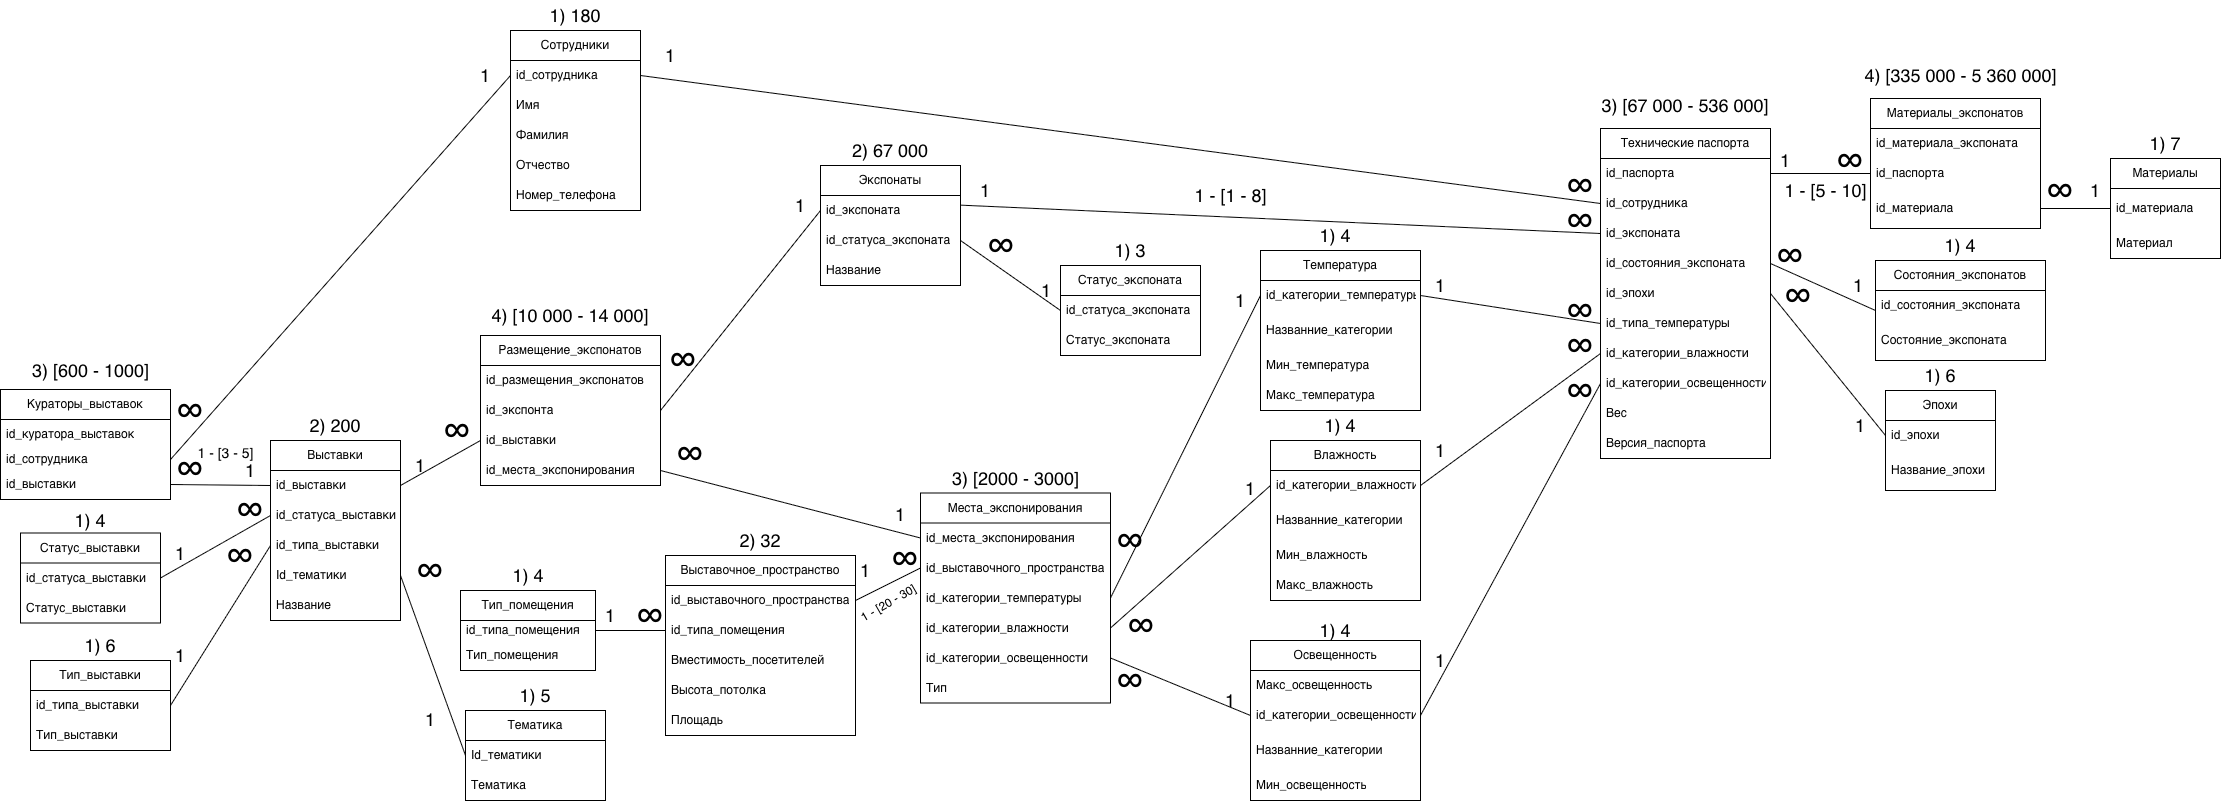
\includegraphics[height=13.5cm]{pic/Схема БД РУС 4.png}
    \caption{Схема базы данных на русском языке}
    \label{db_shema_rus}
\end{figure}

\newpage
\noindent
\vspace{20pt}

\begin{figure}[H]
    \centering
    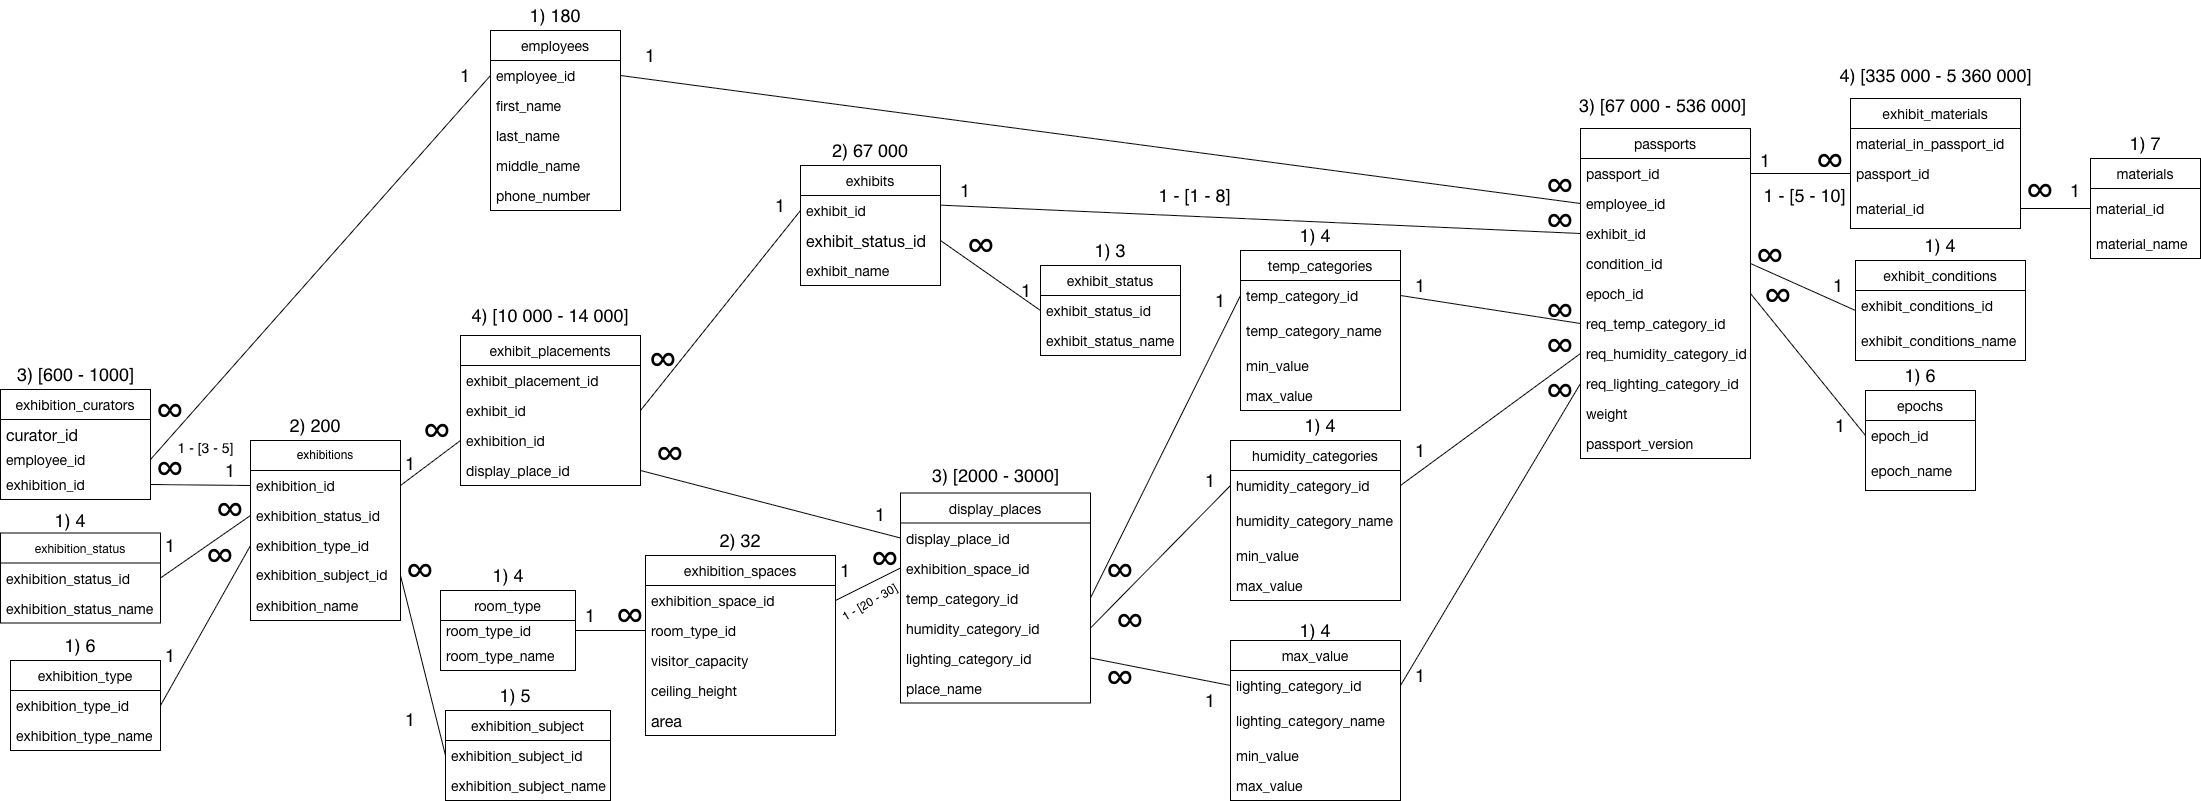
\includegraphics[height=13.5cm]{pic/Схема БД ENG 4.png}
    \caption{Схема базы данных на английском языке}
    \label{db_shema_eng}
\end{figure}

\newpage
\noindent
\vspace{20pt}

\begin{figure}[H]
    \centering
    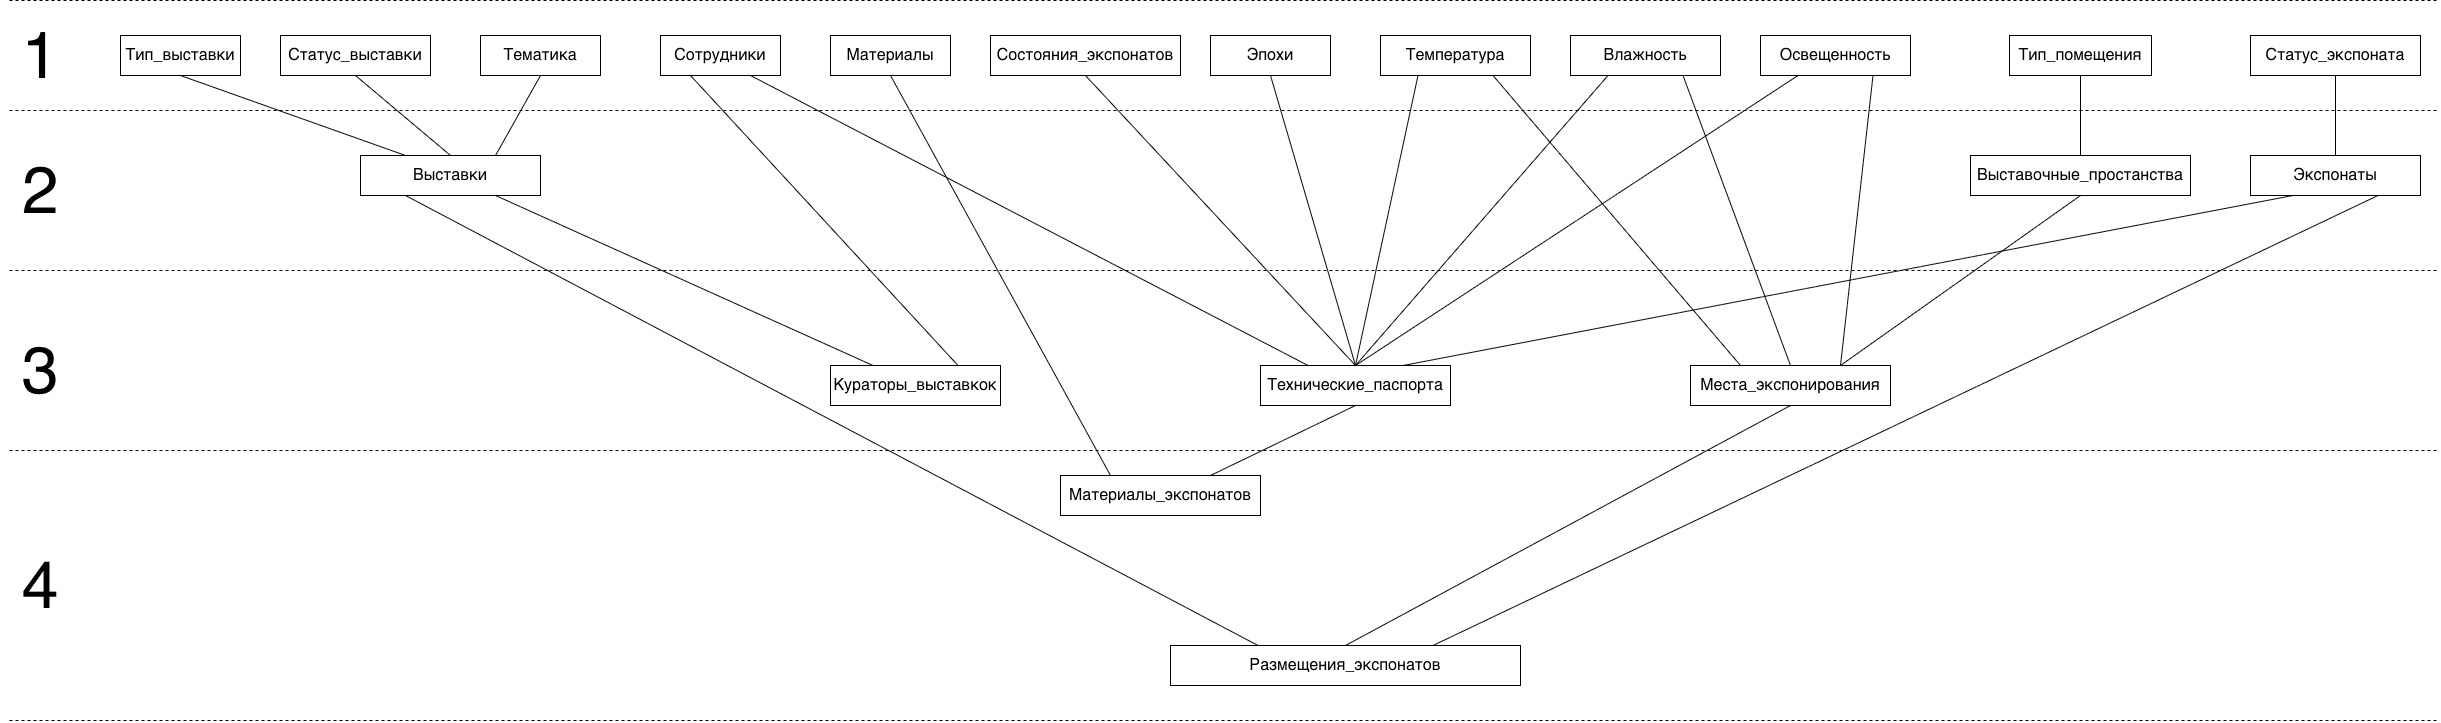
\includegraphics[height=10.5cm]{pic/Уровни заполнения.png}
    \caption{Схема заполнения уровней БД}
    \label{fill_levels}
\end{figure}


\clearpage
\DesigningSavedValues
\recalctypearea
























\iffalse
Программа была реализована на языке C++ c использованием стандартных контейнеров STL, а именно map, string и vector. \par 
Структура проекта представлена на Рис.\ref{structure}.

\begin{figure}[H]
    \centering
    \includegraphics[height=12cm]{pic/structure.jpg}
    \caption{Структура проекта}
    \label{structure}
\end{figure}

\begin{enumerate}
    \item main - точка входа программы.
    \item Exceptions.h - файл с самописными исключениями для использования их в throw - catch
    \item Сonfig.h - файл, в котором задано правило +1.
    \item Interface содержит функции, отвечающие за ввод значений пользователем.
    \item Menu реализует пользовательское меню.
    \item Arithmetic\_class - алгебраическая структура.
    \item Small\_arithmetic.cpp - действия «малой» арифметики.
    \item Big\_arithmetic.cpp - действия «большой» арифметики.
\end{enumerate}


\noindent{\Large \textbf{\subsection{Сonfig.h}}} \par

В Сonfig.h при помощи std::map<char, char> hasse задано правило +1, а также строка-алфавит str\_hasse. 
\begin{lstlisting}[caption=Сonfig.h, label=lst:Сonfig.h]
std::map<char, char> hasse = {
    {'a', 'b'},
    {'b', 'd'},
    {'c', 'a'},
    {'d', 'f'},
    {'e', 'c'},
    {'f', 'i'},
    {'g', 'j'},
    {'h', 'e'},
    {'i', 'k'},
    {'j', 'h'},
    {'k', 'g'}
};

std::string str_hasse = "abcdefghijk";
\end{lstlisting}

\noindent{\Large \textbf{\subsection{Arithmetic\_class.h}}} \par

В Arithmetic\_class.h объявлены методы-действия малой и большой конечной арифметики, а также таблица сложения (с переносами) и умножения (с переносами), которые вычисляются при создании класса Arithmetic, однако далее используются лишь для вывода пользователю, сами вычисления выражений происходят при помощи методов. Также присутствует правило +1 std::map<char, char> hasse, аддитивная единица std::string str\_0 и мультипликативная единица std::string str\_1.

\begin{lstlisting}[caption=Arithmetic\_class.h, label=lst:Arithmetic-class.h]
class  Arithmetic {
public:
    //правило +1
    std::map<char, char> hasse;
    std::string str_hasse;
    //аддитивная единица
    std::string str_0;
    //мультипликативная
    std::string str_1;

    //таблица сложения
    std::vector<std::vector<char>> sum_table;
    //таблица умножения
    std::vector<std::vector<char>> mult_table;

    //таблица переносов при сложении
    std::vector<std::vector<char>> next_sum_table;
    //таблица переносов при умножении
    std::vector<std::vector<char>> next_mult_table;

    Arithmetic(std::map<char, char> input_hasse, std::string input_str_hasse);
    //выделение памяти под таблицы
    void memory_allocation();
    //выводит информацию о калькуляторе
    void print_info();
    //выводит правило +1
    void print_hasse();
    //печать одной любой таблицы
    void print_one_table(std::string title, std::vector<std::vector<char>>& table);
    //печать всех составленных таблиц
    void print_tables();
    //Вывод диапазона чисел
    void print_range();


    //ввод выражений
    void input_action();
    //обработка введенной суммы
    void call_and_out_sum(
        std::string left, std::string right, 
        std::string left_without_minus, std::string right_without_minus,
        int minus_count
    );
    //обработка введенной разности
    void call_and_out_diff(
        std::string left, std::string right, 
        std::string left_without_minus, std::string right_without_minus,
        int minus_count
    );
    //обработка введенного умножения
    void call_and_out_mult(
        std::string left_without_minus, std::string right_without_minus,
        int minus_count
    );
    //обработка введенного частного
    void call_and_out_div(
        std::string left, std::string right, 
        std::string left_without_minus, std::string right_without_minus,
        int minus_count
    );


    //сложение в малой арифметике, возвращает число и перенос в next разряд 
    std::vector<char> small_sum(char left, char right);
    //умножение в малой арфифметике, возвращает число и перенос в next разряд 
    std::vector<char> small_mult(char left, char right);
    //вычитанние в малой арифметике, возвращает число и заем из next разряда 
    std::vector<char> small_diff(char left, char right);
    //деление в малой арифметике, возвращает число и остаток 
    std::vector<char> small_div(char left, char right);


    //сравнение двух чисел, возвращает 1 если left больше, -1 если right больше, 0 если равны
    int compare(std::string left, std::string right);
    //проверяет левое и правое число на 0
    std::vector<bool> find_null(std::string left, std::string right);
    //сложение в большой арифметике
    std::string big_sum(std::string left, std::string right);
    //вычитанние в большой арифметике
    std::string big_diff(std::string left, std::string right);
    //умножение в большой арфифметике
    std::string big_mult(std::string left, std::string right);
    //деление в большой арифметике, возвращает частное и остаток
    std::vector<std::string> big_div(std::string left, std::string right);
};
\end{lstlisting}

\noindent{\Large \textbf{\subsection{Small\_arithmetic.cpp}}} \par

В Small\_arithmetic.cpp реализованы методы вычислений действий «малой» конечной арифметики.
\vspace{8pt}

\textbf{Функция small\_sum } \par
\textbf{Вход:} char left, char right - слагаемые \par
\textbf{Выход:} std::vector<char> result = \{sum, next\} - вектор, содержащий результат суммы и перенос в следующий разряд \par
\textbf{Описание:} Изначально результат суммы равен левому слагаемому, а перенос нулю. Далее к результату суммы и изначально нулевому current\_el начинают одновременно прибвлять единицу в соответствии с правилом +1, пока current\_el не станет равен правому слагаемому. Если во время этого сумма становится равна нулю, то это означает обнуление разряда, значение переноса при этом увеличивается на единицу.\par
\vspace{10pt}

\textbf{Функция small\_mult } \par
\textbf{Вход:} char left, char right - множители \par
\textbf{Выход:} std::vector<char> result = \{mult, next\} - вектор, содержащий результат произведения и перенос в следующий разряд \par
\textbf{Описание:} Изначально результат произведения равен левому слагаемому, а перенос нулю. Далее происходит проверка умножения на ноль, при котором и произведение, и перенос равны нулю. Умножение left*right можно представить как сложение left с самим собой right-1 раз, поэтому к mult прибавляется right, пока current\_el не станет равен right-1, при этом перенос умножения равен сумме всех переносов этих сложений.\par
\vspace{10pt}

\begin{lstlisting}[caption=small\_sum и small\_mult, label=lst:small-sum и small-mult]
//сложение в малой арифметике, возвращает число и перенос в next разряд 
std::vector<char> Arithmetic::small_sum(char left, char right){
    //левое слагаемое будем двигать, пока не достигнем суммы
    char sum = left;
    //по умолчанию перенос равен нулю
    char next = str_hasse[0];

    //будем делать +1 у левого, пока current_el = 0 не сравняется с right
    char current_el = str_hasse[0];
    while(current_el != right){
        current_el = hasse[current_el];

        sum = hasse[sum];
        // <=> обнулению круга
        if(sum == str_hasse[0]) next = hasse[next];
    }

    std::vector<char> result = {sum, next};
    return result;
}

//умножение в малой арфифметике, возвращает число и перенос в next разряд 
std::vector<char> Arithmetic::small_mult(char left, char right){
    //левое слагаемое будем двигать, пока не достигнем произведения
    char mult = left;
    //по умолчанию перенос равен нулю
    char next = str_hasse[0];

    //умножение на ноль
    if(left == str_hasse[0] || right == str_hasse[0]){
        std::vector<char> result = {str_hasse[0], str_hasse[0]};
        return result;
    }

    //умножение - это прибовление к left числа left right-1 раз
    char current_el = str_hasse[0];
    while(hasse[current_el] != right){ // <=> right-1 раз
        current_el = hasse[current_el];

        std::vector<char> sum_i = small_sum(mult, left);
        mult = sum_i[0];
        //к переносу умножения пребавляем перенос i-ой суммы
        next = small_sum(next, sum_i[1])[0];
    }

    std::vector<char> result = {mult, next};
    return result;
}
\end{lstlisting}

\textbf{Функция small\_diff } \par
\textbf{Вход:} char left - уменьшаемое, char right - вычитаемое \par
\textbf{Выход:} std::vector<char> result = \{diff, next\} - вектор, содержащий результат разности и заем из следующего разряда \par
\textbf{Описание:} Разность вычисляется как действие, обратное сложению. Изначально разность равна нулю. Далее ее увеличивают, пока сумма diff+rigth не становится равной left. При этом значения заема разности совпадает с переносом этой суммы.\par
\vspace{10pt}

\textbf{Функция small\_div } \par
\textbf{Вход:} char left - делимое, char right - делитель \par
\textbf{Выход:} std::vector<char> result = \{div, remain\} - вектор, содержащий результат деления и остаток \par
\textbf{Описание:} Деление вычисляется как действие, обратное умножению. Изначально частное и остаток равны нулю. Далее остаток remain увеличивают, пока он не станет равным делителю right, после чего он сбрасывается до нуля, а частное увеличивается на единицу. Это продолжается пока div * right + remain не сравняется с делимым left.\par
\vspace{10pt}

\begin{lstlisting}[caption=small\_diff и small\_div, label=lst:small-diff и small-div]
//вычитанние в малой арифметике, возвращает число и заем из next разряда 
std::vector<char> Arithmetic::small_diff(char left, char right){
    //a - b = c <=> с + b = a
    //будем двигать разность, пока не найдем вычитаемое
    char diff = str_hasse[0];
    std::vector<char> result;

    std::vector<char> sum_i;
    do{
        sum_i = small_sum(diff, right);
        //заем совпадает с переносом при сумме
        result = {diff, sum_i[1]};
        diff = hasse[diff]; 
    } while(sum_i[0] != left);

    return result;
}

//деление в малой арифметике, возвращает число и остаток 
std::vector<char> Arithmetic::small_div(char left, char right){
    //(a - ост) / b = c <=> a = b*c + ост,  ост < b
    //будем двигать частное и остаток для каждого частного, пока не найдем делимое
    char div = str_hasse[0];
    char remain = str_hasse[0]; //остаток
    std::vector<char> result;

    std::vector<char> sum_i;
    std::vector<char> mult_i;
    do{
        mult_i = small_mult(right, div);
        sum_i = small_sum(mult_i[0], remain);

        result = {div, remain};

        remain = hasse[remain];
        //если остаток сравнялся с делителем
        if(remain == right){
            //сбрасываем остаток и двигаем частное
            remain = str_hasse[0];
            div = hasse[div];
        }
    } while(sum_i[0] != left);

    return result;
}
\end{lstlisting}

\newpage

\noindent{\Large \textbf{\subsection{Big\_arithmetic.cpp}}} \par
В Big\_arithmetic.cpp реализованы методы вычислений действий «большой» конечной арифметики. \par
Для начала рассмотрим два вспомогательных метода. 
\vspace{8pt}

\textbf{Функция compare } \par
\textbf{Вход:} std::string left, std::string right - числа, которые требуется сравнить\par
\textbf{Выход:} int result, причем он равен -1 при left < right, равен 1 при left > right и равен 0 при left = right\par
\textbf{Описание:} В начале у чисел убираются незначащие нули. После этого уже можно считать, что число с большим числом разрядов больше другого. Если же числа равны по числу разрядов, то происходит поразрядное сравнение, начиная со старшего разряда, при котором изначально нулевые счетчики увеличиваются на единицу, пока не достигнут значения соответствующего разряда у левого или правого числа. При этом, если один из счетчиков не успел увеличится до соотв. разряда, а другой успел, то это значит, что число, в котором счетчик успел совпасть, меньше другого. Если же все разряды чисел совпали, то числа считаются равными, возвращается result = 0. \par
\vspace{10pt}

\textbf{Функция find\_null } \par
\textbf{Вход:} std::string left, std::string right - числа, которые требуется проверить на равенство нулю \par
\textbf{Выход:} std::vector<bool> result = \{left\_is\_zero, right\_is\_zero\} - вектор с результатами проверки равенства нулю для левого и правого числа\par
\textbf{Описание:} Происходит поразрядный перебор каждого числа. Если находится хотя бы один ненулевой разряд в числе, то результатом проверки возвращается false для этого числа. \par
\vspace{10pt}

\begin{lstlisting}[caption=compare и find\_null, label=lst:compare и find-null]
//сравнение двух чисел, возвращает 1 если left больше, -1 если right больше, 0 если равны
int Arithmetic::compare(std::string left, std::string right){
    //убираем незначащие нули
    while(left.size() > 1 && left[0] == str_hasse[0]) left = left.substr(1);
    while(right.size() > 1 && right[0] == str_hasse[0]) right = right.substr(1);

    //если длины разные, то больше то число, у которого длина больше
    if(left.size() > right.size()) return 1;
    if(left.size() < right.size()) return -1;

    //если длины равны, сравниваем поразрядно
    for(int i = 0; i < left.size(); i++){
        //сдвигаем от нуля до left[i] и right[i]
        char current_left_i = str_hasse[0];
        char current_right_i = str_hasse[0];
        while(current_left_i != left[i] && current_right_i != right[i]){
            current_left_i = hasse[current_left_i];
            current_right_i = hasse[current_right_i];
        }
        //кто успел до себя допрыгать, тот и меньше
        if(current_left_i == left[i] &&  current_right_i != right[i]) return -1;
        if(current_left_i != left[i] &&  current_right_i == right[i]) return 1;
    }

    //числа равны
    return 0;
}

//проверяет левое и правое число на 0
std::vector<bool> Arithmetic::find_null(std::string left, std::string right){
    bool left_is_zero = true;
    for(int i = 0; i < left.size(); i++){
        if(left[i] != str_hasse[0]){
            left_is_zero = false;
            break;
        }
    }

    bool right_is_zero = true;
    for(int i = 0; i < right.size(); i++){
        if(right[i] != str_hasse[0]){
            right_is_zero = false;
            break;
        }
    }

    std::vector<bool> result = {left_is_zero, right_is_zero};
    return result;
}
\end{lstlisting}

\textbf{Функция big\_sum } \par
\textbf{Вход:} std::string left, std::string right - слагаемые\par
\textbf{Выход:} std::string sum - результат суммы чисел\par
\textbf{Описание:} В начале у чисел убираются незначащие нули. После этого числа переворачиваются для суммирования, начиная с младших разрядов. Суммирование продолжается, пока не достигается старший разряд хотя бы одного из чисел или если есть перенос из текущего разряда. Если же порядок старшего разряда числа меньше, чем у текущего суммируемого разряда, то ему приписывается значение нуля. Суммирование разрядов и вычисление переноса осуществляется при помощи описанного выше метода small\_sum, значение суммы для разряда добавляется к результату sum. Так как суммирование происходит, начиная с младших разрядов, то результат необходимо перевернуть. Если после суммирования получилось число, у которого больше 8 разрядов, то вызывается исключение с сообщением о переполнении.\par
\vspace{10pt}

\textbf{Функция big\_mult } \par
\textbf{Вход:} std::string left, std::string right - множители \par
\textbf{Выход:} std::string mult - результат произведения чисел\par
\textbf{Описание:} В начале у чисел убираются незначащие нули. После этого происходит проверка чисел на равенство нулю при помощи описанного выше метода find\_null. Если хотя бы одно из них является нулем, то и произведение равно нулю. Если же оба числа ненулевые, то они переворачиваются для умножения, начиная с младших разрядов. При вычислениях столбиком, число left поочередно умножается на каждый разряд числа right (умножаются разряды left, при этом учитываются переносы), при помощи описанного выше метода small\_mult. Каждое такое произведение переворачивается и происходит сдвиг на порядок соответствующего рязряда right. Такой результат произведения для каждого разряда right прибавляется к итоговому mult при помощи big\_sum. Если результатом произведения получилось число, у которого больше 8 разрядов, то вызывается исключение с сообщением о переполнении. \par
\vspace{10pt}

\begin{lstlisting}[caption=big\_sum и big\_mult, label=lst:big-sum и big-mult]
//сложение в большой арифметике
std::string Arithmetic::big_sum(std::string left, std::string right){
    std::string sum = "";
    //нужно убрать незначащие нули, потому что иначе программа падает
    while(left.size() > 1 && left[0] == str_hasse[0]) left = left.substr(1);
    while(right.size() > 1 && right[0] == str_hasse[0]) right = right.substr(1);

    int i = 0;
    int j = 0;

    //переворачиваем строки для суммирования от младших разрядов
    std::reverse(left.begin(), left.end());
    std::reverse(right.begin(), right.end());

    char next = str_hasse[0];
    while(i < left.size() || j < right.size() || next != str_hasse[0]){
        char left_i = (i < left.size()) ? left[i] : str_hasse[0];
        char right_j = (j < right.size()) ? right[j] : str_hasse[0];

        //вначале к первому числу прибавим перенос от предыдущей суммы
        std::vector<char> add_next = small_sum(left_i, next);
        left_i = add_next[0];
        next = add_next[1];

        std::vector<char> sum_i = small_sum(left_i, right_j);
        sum += sum_i[0];
        next = small_sum(sum_i[1], next)[0];
        i++;
        j++;
    }
    
    //убираем незначащие нули
    std::reverse(sum.begin(), sum.end());
    while(sum.size() > 1 && sum[0] == str_hasse[0]) sum = sum.substr(1);
    if(sum.size() > 8) throw Input_error("При вычислениях произошло переполнение разрядов!");
    return sum;
}

//умножение в большой арфифметике
std::string Arithmetic::big_mult(std::string left, std::string right){
    std::string mult = "";
    mult += str_hasse[0];

    //нужно убрать незначащие нули, потому что иначе программа падает
    while(left.size() > 1 && left[0] == str_hasse[0]) left = left.substr(1);
    while(right.size() > 1 && right[0] == str_hasse[0]) right = right.substr(1);

    //умножение на 0
    std::vector<bool> nulls = find_null(left, right);
    if(nulls[0] || nulls[1]) return mult;

    //переворачиваем строки для умножения от младших разрядов
    std::reverse(left.begin(), left.end());
    std::reverse(right.begin(), right.end());

    //умножение столбиком
    int j = 0;
    while(j < right.size()){
        //берем разряд второго множителя
        char right_j = right[j];
        
        //произведение для текущего разряда
        std::string tmp_mult = "";
        char next = str_hasse[0];
        
        int i = 0;
        while(i < left.size() || next != str_hasse[0]){
            char left_i = (i < left.size()) ? left[i] : str_hasse[0];

            //умножаем текущий разряд left на текущий разряд right
            std::vector<char> mult_i = small_mult(left_i, right_j);
            
            //добавляем перенос от предыдущего умножения
            std::vector<char> add_next = small_sum(mult_i[0], next);
            tmp_mult += add_next[0];
            next = small_sum(mult_i[1], add_next[1])[0];
            
            i++;
        }

        //переворачиваем tmp_mult обратно и добавляем сдвиг нулями справа
        std::reverse(tmp_mult.begin(), tmp_mult.end());
        for(int k = 0; k < j; k++){
            tmp_mult += str_hasse[0];
        }

        //добавляем к общему результату
        mult = big_sum(mult, tmp_mult);
        
        j++;
    }

    //убираем незначащие нули, если есть
    while(mult.size() > 1 && mult[0] == str_hasse[0]) mult = mult.substr(1);

    if(mult.size() > 8) throw Input_error("При вычислениях произошло переполнение разрядов!");

    return mult;
}
\end{lstlisting}

\textbf{Функция big\_diff } \par
\textbf{Вход:} std::string left - уменьшаемое, std::string right - вычитаемое\par
\textbf{Выход:} std::string diff - результат разности чисел\par
\textbf{Описание:} В начале у чисел убираются незначащие нули. После этого числа переворачиваются для вычитания, начиная с младших разрядов. Вычитание продолжается, пока не достигается старший разряд хотя бы одного из чисел. Если же порядок старшего разряда числа меньше, чем у текущего суммируемого разряда, то ему приписывается значение нуля. Вычитание разрядов и вычисление заема осуществляется при помощи описанного выше метода small\_diff, значение разности для разряда добавляется к результату diff. Так как вычитание происходит, начиная с младших разрядов, то результат необходимо перевернуть. Если после вычитания получилось число, у которого больше 8 разрядов, то вызывается исключение с сообщением о переполнении.\par
\vspace{10pt}

\textbf{Функция big\_div } \par
\textbf{Вход:} std::string left - делимое, std::string right - делитель \par
\textbf{Выход:} std::vector<std::string> result = \{div, remain\} - вектор, содержащий значение частного и остатка\par
\textbf{Описание:} В начале происходит проверка чисел на равенство нулю при помощи метода find\_null. Если оба числа равны нулю, то выводится весь диапазон чисел (для варианта D2 это $[-cccccccc, +cccccccc]$). Если только делитель равен нулю, то выводится пустое множество «Ø». Если только делимое равно нулю, то частное и остаток равны нулю. Далее у чисел убираются незначащие нули. Деление реализовано подбором значений частного div и остатка remain. Происходит увеличение остатка на единицу, пока он не сравняется с делителем. Когда остаток становится равен делителю, то его значение сбрасывается до нуля, а частное увеличивается на единицу. Это продолжается, пока $right * div + remain \not= left$.\par
\vspace{10pt}

\begin{lstlisting}[caption=big\_diff и big\_div, label=lst:big-diff и big-div]
//вычитанние в большой арифметике
std::string Arithmetic::big_diff(std::string left, std::string right){
    //нужно убрать незначащие нули, потому что иначе программа падает
    while(left.size() > 1 && left[0] == str_hasse[0]) left = left.substr(1);
    while(right.size() > 1 && right[0] == str_hasse[0]) right = right.substr(1);

    //переворачиваем строки для вычитания от младших разрядов
    std::reverse(left.begin(), left.end());
    std::reverse(right.begin(), right.end());

    std::string diff = "";
    int i = 0;
    int j = 0;

    char next = str_hasse[0];
    while(i < left.size() || j < right.size()){
        char left_i = (i < left.size()) ? left[i] : str_hasse[0];
        char right_j = (j < right.size()) ? right[j] : str_hasse[0];

        //вначале из первого числа вычтем заем от предыдущей разности
        std::vector<char> diff_next = small_diff(left_i, next);
        left_i = diff_next[0];
        next = diff_next[1];

        std::vector<char> diff_i = small_diff(left_i, right_j);
        diff += diff_i[0];
        next = small_sum(diff_i[1], next)[0];
        i++;
        j++;
    }

    //убираем незначащие нули
    std::reverse(diff.begin(), diff.end());
    while(diff.size() > 1 && diff[0] == str_hasse[0]) diff = diff.substr(1);

    if(diff.size() > 8) throw Input_error("При вычислениях произошло переполнение разрядов!");

    return diff;
}

//деление в большой арифметике, возвращает частное и остаток
std::vector<std::string> Arithmetic::big_div(std::string left, std::string right){
    //проверка a/0 и 0/0
    std::vector<bool> nulls = find_null(left, right);

    if(nulls[0] && nulls[1]){
        print_range();
        throw Input_error("");
    }
    if(nulls[1]){
        std::cout << "Результат: Ø\n";
        throw Input_error("");
    }
    if(nulls[0]){
        std::vector<std::string> result = {str_0, str_0};
        return result;
    }

    //нужно убрать незначащие нули, потому что иначе программа падает
    while(left.size() > 1 && left[0] == str_hasse[0]) left = left.substr(1);
    while(right.size() > 1 && right[0] == str_hasse[0]) right = right.substr(1);
    
    std::string div = str_0;
    std::string remain = str_0;

    std::string sum_i;
    std::string mult_i;

    //a = bc + ост, ост < b
    //будем двигать частное и остаток для каждого частного, пока не найдем делимое
    do{
        mult_i = big_mult(right, div);
        sum_i = big_sum(mult_i, remain);

        if(compare(sum_i, left) == 0) break;

        //увеличиваем остаток на 1
        remain = big_sum(remain, str_1);

        if(compare(remain, right) == 0){
            //сбрасываем остаток и двигаем частное
            remain = str_0;
            div = big_sum(div, str_1);
        }
    } while(true);

    //убираем незначащие нули из частного
    while(div.size() > 1 && div[0] == str_hasse[0]) div = div.substr(1);
    //убираем незначащие нули из остатка
    while(remain.size() > 1 && remain[0] == str_hasse[0]) remain = remain.substr(1);

    std::vector<std::string> result = {div, remain};
    return result;
}
\end{lstlisting}



\noindent{\Large \textbf{\subsection{Обработка ввода чисел}}} \par
Описанные выше функции для действий «большой» конечной арифметики работают лишь для двух неотрицательных чисел, поэтому необходимо дополнительно обрабатывать вводимые пользователем числа для работы с отрицательными числами. \par
\vspace{10pt}

\textbf{Функция call\_and\_out\_sum } \par
\textbf{Вход:} std::string left, std::string right - числа, введенные пользователем; std::string left\_without\_minus, std::string right\_without\_minus - эти же числа, но гарантированно неотрицательные; int minus\_count - количество введенных отрицательных чисел (0 если оба неотрицательны, 1 если одно отрицательно, 2 если оба отрицательны)\par
\textbf{Выход:} результат суммирования с учетом знаков\par
\textbf{Описание:} Если оба введенных числа неотрицательные, то вызывается суммирование двух неотрицательных чисел big\_sum. Если же оба числа являются отрицательными, то снова вызывается big\_sum, но уже гарантированно для чисел без минусов, а к значению результата приписывается минус (если это не нуль). Суммирование двух чисел, одно из которых отрицательно, можно вычислить как разность двух неотрицательных чисел, поэтому после определения отрицательного числа (его исходная длина не совпадает с длиной без знака «-»), вызывается обработка разности, где на место вычитаемого ставится изначально отрицательное число без минуса.\par
\vspace{10pt}

\textbf{Функция call\_and\_out\_diff } \par
\textbf{Вход:} std::string left, std::string right - числа, введенные пользователем; std::string left\_without\_minus, std::string right\_without\_minus - эти же числа, но гарантированно неотрицательные; int minus\_count - количество введенных отрицательных чисел \par
\textbf{Выход:} результат вычитания с учетом знаков\par
\textbf{Описание:} Если оба введенных числа неотрицательные, то происходит поиск большего из них при помощи compare, потому что значение, вычисленное big\_diff может быть только положительным. Если left < right, то вычисляется big\_diff, в котором left и right поменяны местами, а к результату приписывается минус. Если же left $\geq$ right, то аргументами big\_diff являются числа в том же порядке. Случай, когда оба введенных числа оказываются отрицательными, можно рассматривать как -left - -right = right - left (разность двух неотрицательных чисел). Случай, когда только правое число отрицательно, можно рассматривать как сложение двух неотрицательных чисел. Случай, когда только левое число отрицательное можно рассматривать как \\ -left - right = -(left+right).\par
\vspace{10pt}

\begin{lstlisting}[caption=call\_and\_out\_sum и call\_and\_out\_diff, label=lst:call-and-out-sum и call-and-out-diff]
//обработка введенной суммы
void Arithmetic::call_and_out_sum(
    std::string left, std::string right, 
    std::string left_without_minus, std::string right_without_minus,
    int minus_count
){
    bool is_sum = true;
    std::string result;
    switch (minus_count){
        case 0:
            result = big_sum(left, right);
            break;
        case 2:
            result = big_sum(left_without_minus, right_without_minus);
            if(result != str_0) result = "-" + result;
            break;
        case 1:
            //<=> правое число отрицательное
            if(right.size() != right_without_minus.size()){
                call_and_out_diff(left_without_minus, right_without_minus, left_without_minus, right_without_minus, 0);
            }
            else{ 
                call_and_out_diff(right_without_minus, left_without_minus, right_without_minus, left_without_minus, 0);
            }
            is_sum = false; //чтобы дважды результат не выводило
            break;
        default:
            break;
    }

    if(is_sum) std::cout << "Результат: " << result << "\n\n";
}

//обработка введенной разности
void Arithmetic::call_and_out_diff(
    std::string left, std::string right, 
    std::string left_without_minus, std::string right_without_minus,
    int minus_count
){
    std::string result;
    switch (minus_count){
        case 0:
            if(compare(left, right) == -1){ //если правое больше
                result = big_diff(right, left);
                if(result != str_0) result = "-" + result;
            } else{
                result = big_diff(left, right);
            }
            break;
        case 2: // -a - -b = b - a
            if(compare(right_without_minus, left_without_minus) == -1){ //если a > b
                result = big_diff(left_without_minus, right_without_minus);
                if(result != str_0) result = "-" + result;
            } else{
                result = big_diff(right_without_minus, left_without_minus);
            }
            break;
        case 1:
            //<=> правое число отрицательное
            if(right.size() != right_without_minus.size()) result = big_sum(left, right_without_minus);
            else{ 
                result = big_sum(left_without_minus, right);
                if(result != str_0) result = "-" + result;
            }
            break;
        default:
            break;
    }

    std::cout << "Результат: " << result << "\n\n";
}
\end{lstlisting}

\textbf{Функция call\_and\_out\_mult } \par
\textbf{Вход:} std::string left, std::string right - числа, введенные пользователем; std::string left\_without\_minus, std::string right\_without\_minus - эти же числа, но гарантированно неотрицательные; int minus\_count - количество введенных отрицательных чисел\par
\textbf{Выход:} результат умножения с учетом знаков\par
\textbf{Описание:} При умножении можно считать значение произведения big\_mult для двух гарантированно неотрицательных чисел, а после приписывать к нему «-» (если это не нуль), если только одно из введенных чисел отрицательно.\par
\vspace{10pt}

\textbf{Функция call\_and\_out\_div } \par
\textbf{Вход:} std::string left, std::string right - числа, введенные пользователем; std::string left\_without\_minus, std::string right\_without\_minus - эти же числа, но гарантированно неотрицательные; int minus\_count - количество введенных отрицательных чисел \par
\textbf{Выход:} результат деления и остаток с учетом знаков\par
\textbf{Описание:} В начале вычисляется частное и остаток при помощи big\_div для двух гарантированно неотрицательных чисел (это и является результатом вычислений, если пользователь не ввел отрицательных чисел, или если оба числа оказались отрицательными). Если только делитель отрицательный, то достаточно просто приписать «-» частному, а остаток трогать не нужно. Если же только делимое отрицательно, то частное необходимо увеличить на единицу (т.к. далее к нему припишется «-», то это эквивалентно уменьшению на один), а далее подобрать новый остаток для которого выполнится $left = (div-1) * right + new\_remain$.\par
\vspace{10pt}

\begin{lstlisting}[caption=call\_and\_out\_mult и call\_and\_out\_div, label=lst:call-and-out-mult и call-and-out-div]
//обработка введенного умножения
void Arithmetic::call_and_out_mult(
    std::string left_without_minus, std::string right_without_minus,
    int minus_count
){
    std::string result;
    result = big_mult(left_without_minus, right_without_minus);
    if(minus_count == 1 && result != str_0) result = "-" + result;

    std::cout << "Результат: " << result << "\n\n";
}

//обработка введенного частного
void Arithmetic::call_and_out_div(
    std::string left, std::string right, 
    std::string left_without_minus, std::string right_without_minus,
    int minus_count
){
    std::vector<std::string> result = big_div(left_without_minus, right_without_minus);

    if(minus_count == 1){
        //<=> отрицательное левое нужно по особому отработать (если остаток не 0); если только правое, то просто "-" допишем к частному
        if(left.size() != left_without_minus.size() && result[0] != str_0){
            //если остаток не ноль
            if(result[1] != str_0){
                //уменьшим частное на 1 (по модулю)
                result[0] = big_sum(result[0], str_1);
                //подбираем остаток для нового частного
                result[1] = str_0;
                //a != (div-1) * b + new_remain
                std::string new_left = big_mult(result[0], right_without_minus);
                while( compare(left_without_minus, big_diff(new_left, result[1]) ) != 0 ){
                    result[1] = big_sum(result[1], str_1);
                }
            }
        }

        //ну мало ли
        if((result[0]).size() > 8) throw Input_error("При вычислениях произошло переполнение разрядов!");
        //дописываем минус частному
        if(result[0] != str_0) result[0] = "-" + result[0];
    }

    std::cout << "Частное: " << result[0] << "\n";
    std::cout << "Остаток: " << result[1] << "\n\n";
}
\end{lstlisting}
\fi
\newpage


%Программирование
\noindent
{\Large \textbf{\section{Программирование}}} \par
\noindent
\vspace{-40pt}

{\Large \textbf{\subsection{Заполнение базы данных}}} \par

Код создания таблиц для базы данных приведен в приложении А. Код для генерации данных был написан на языке Python, он приведен в приложении Б. 
Количество записей в сгенерированных таблицах представлено в таблице \ref{kolvo}.

\begin{table}[htbp]
\centering
\label{tab:db_records_count_grid}
\begin{tabular}{|l|r|}
\hline
\textbf{Название таблицы} & \textbf{Количество записей} \\ \hline
exhibit\_materials     & 2 261 727 \\ \hline
passports              &   301 374 \\ \hline
exhibits               &    67 000 \\ \hline
exhibit\_placements    &    12 196 \\ \hline
display\_places        &     2 535 \\ \hline
exhibition\_curators   &        781 \\ \hline
exhibitions            &        200 \\ \hline
employees              &        180 \\ \hline
exhibition\_spaces     &        100 \\ \hline
materials              &         63 \\ \hline
epochs                 &          6 \\ \hline
exhibition\_type       &          6 \\ \hline
exhibition\_subject    &          5 \\ \hline
exhibit\_conditions    &          5 \\ \hline
room\_type             &          4 \\ \hline
humidity\_categories   &          4 \\ \hline
exhibition\_status     &          4 \\ \hline
temp\_categories       &          4 \\ \hline
exhibit\_status        &          4 \\ \hline
lighting\_categories   &          4 \\ \hline
\textbf{ВСЕГО ЗАПИСЕЙ В БД} & \textbf{2 646 202} \\ \hline
\end{tabular}
\caption{Количество записей в таблицах базы данных}
\label{kolvo}
\end{table}

\vspace{-40pt}

{\Large \textbf{\subsection{Запросы}}} \par

Лист проверки выполнения запросов представлен на Рис.\ref{queriesscreen}.

\begin{figure}[H]
    \centering
    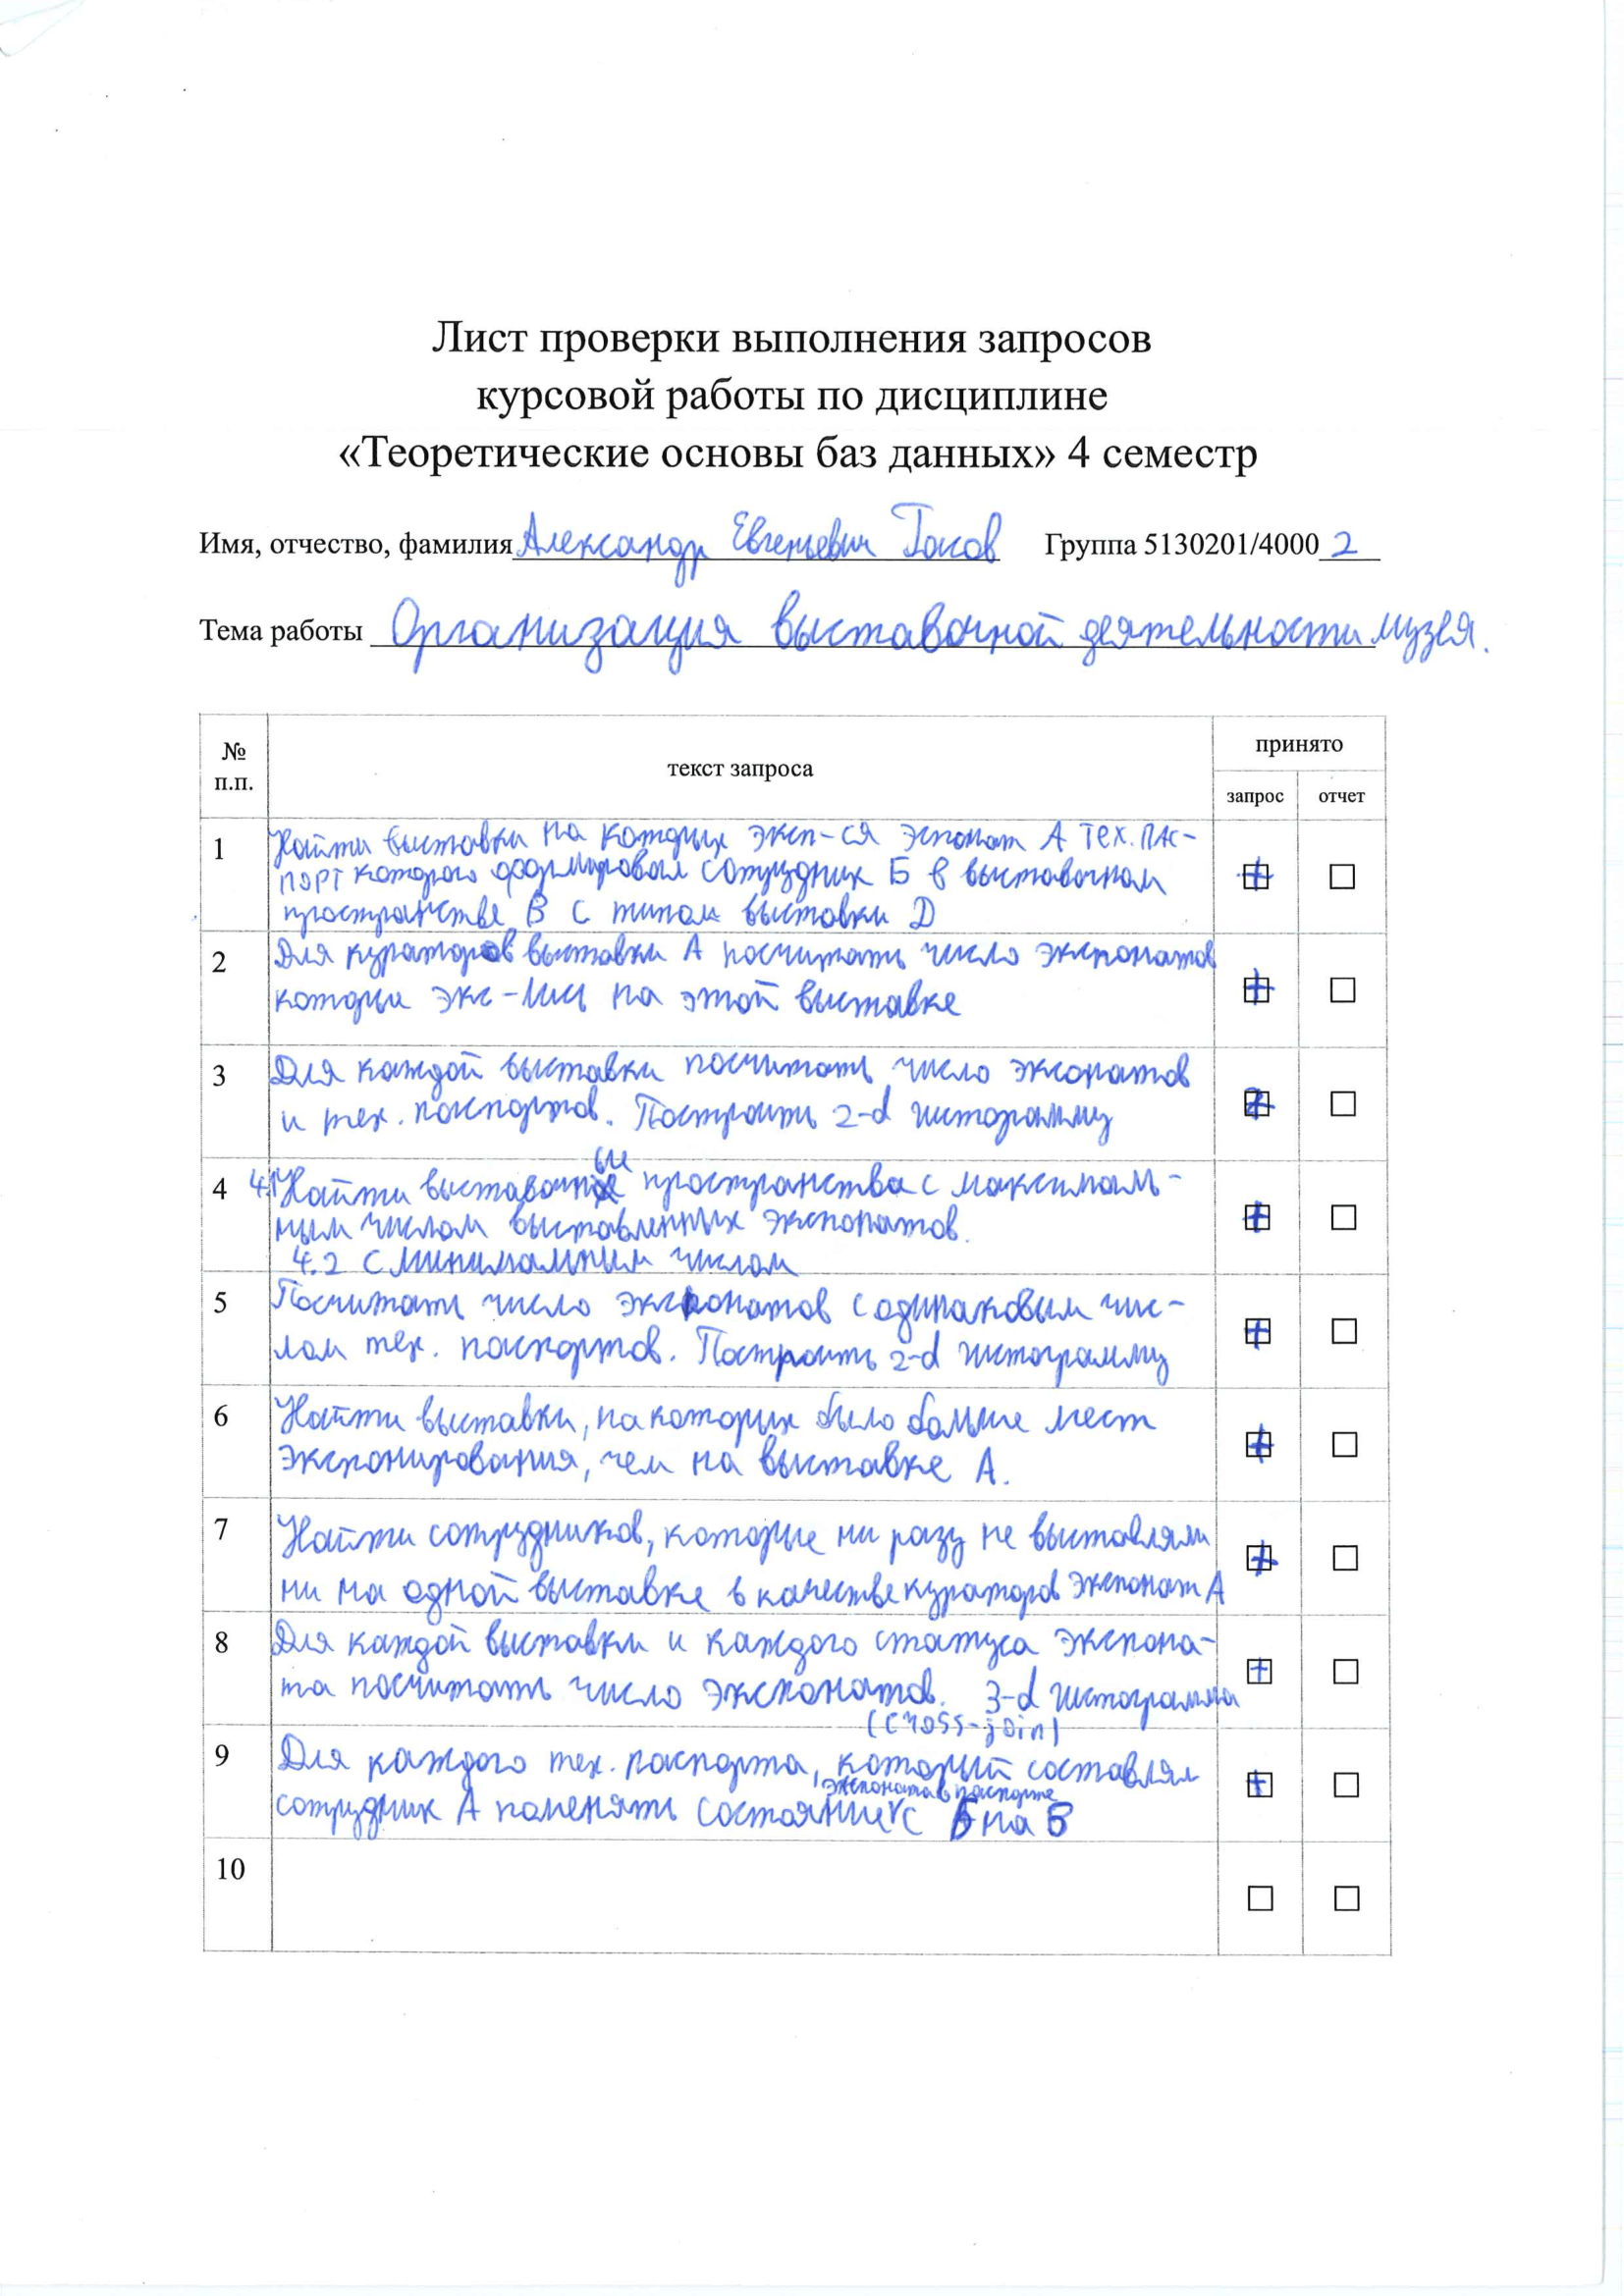
\includegraphics[width=\textwidth,height=0.90\textheight,keepaspectratio]{pic/queriesscreen.png}
    \caption{Лист проверки выполнения запросов}
    \label{queriesscreen}
\end{figure}

Для анализа запросов использовалась команда \texttt{EXPLAIN ANALYZE}. Время планирования и выполнения запросов приведено в таблице~\ref{tab:query-time}. \par

\begin{table}[H]
\centering
{\small
\begin{tabular}{|c|c|c|}
\hline
Запрос  & Planning Time, мс & Execution Time, мс \\
\hline
1 & 0.567 & 17.300 \\
\hline
2 & 0.665 & 12.473 \\
\hline
3 & 0.090 & 41.806 \\
\hline
4.1  & 0.104 & 7.288 \\
\hline
4.2  & 0.281 & 9.731 \\
\hline
5  & 0.095 & 64.808 \\
\hline
6  & 0.067 & 3.646 \\
\hline
7  & 0.174 & 2.170 \\
\hline
8  & 0.129 & 69.868 \\
\hline
9  & 0.062 & 28.464 \\
\hline
\end{tabular}}
\caption{Время планирования и выполнения запросов}
\label{tab:query-time}
\end{table}

Визуализации планов выполнения запросов были построены с помощью
сервиса explain.dalibo.com \cite{site:explain}.

\subsection{Запрос 1}

Найти выставки, на которых экспонируется экспонат А, технический паспорт которого формировал сотрудник Б, в выставочном пространстве В с типом выставки Д. Текст запроса представлен в Листинге~\ref{lst:q1}. \par

\lstinputlisting[language=SQL, caption={Запрос 1}, label={lst:q1}, basicstyle=\ttfamily\footnotesize]{../../../queries/q1.sql}

Реляционная формула запроса:
\[
\begin{gathered}
R_1 = 
\pi_{\text{exhibition\_name}}
\left(
\sigma_{\substack{
\text{exhibit\_name}=A \ \land \\
\text{employee}=B \ \land \\
\text{room\_type\_name}=C \ \land \\
\text{exhibition\_type\_name}=D
}}
\left(
\begin{gathered}
\text{exhibitions} 
\bowtie_{\text{exhibition\_id}} \\
\text{exhibit\_placements} 
\bowtie_{\text{exhibit\_id}} \\
\text{exhibits} 
\bowtie_{\text{exhibit\_id}} \\
\text{passports} 
\bowtie_{\text{employee\_id}} \\
\text{employees} 
\bowtie_{\text{display\_place\_id}} \\
\text{display\_places} 
\bowtie_{\text{exhibition\_space\_id}} \\
\text{exhibition\_spaces} 
\bowtie_{\text{room\_type\_id}} \\
\text{room\_type} 
\bowtie_{\text{exhibition\_type\_id}} \\
\text{exhibition\_type}
\end{gathered}
\right)
\right), \\
\text{где } \bowtie \text{ --- это natural join}
\end{gathered}
\]

Результат выполнения запроса 1 (выведены первые 20 строк) представлен на Рис.\ref{fig:q1-result}. \par

\begin{figure}[H]
    \centering
    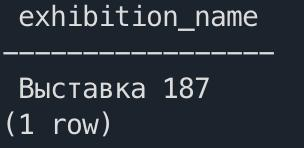
\includegraphics[width=\textwidth,height=3cm,keepaspectratio]{pic/q1.jpg}
    \caption{Результат выполнения запроса 1 (выведены первые 20 строк)}
    \label{fig:q1-result}
\end{figure}

План выполнения запроса 1 представлен на Рис.\ref{fig:q1-explain}. \par

\begin{figure}[H]
    \centering
    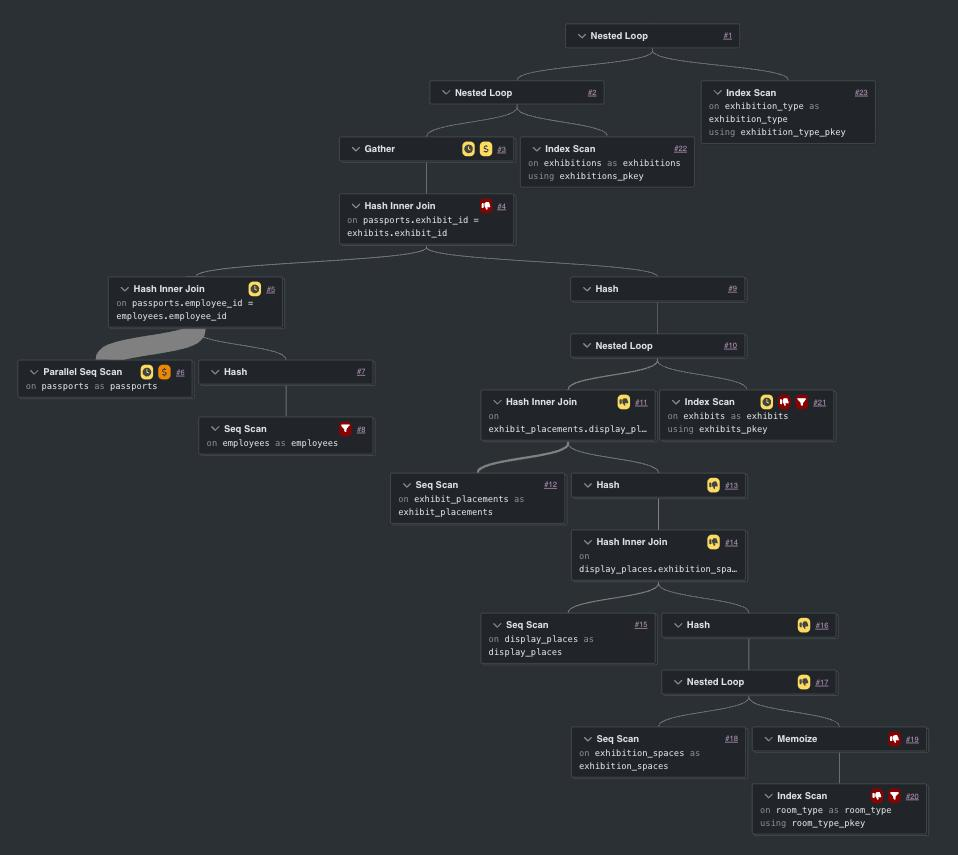
\includegraphics[width=\textwidth,height=0.75\textheight,keepaspectratio]{pic/exp1.jpg}
    \caption{План выполнения запроса 1}
    \label{fig:q1-explain}
\end{figure}

В плане выполнения запроса последовательно соединяются таблицы выставок, размещений, экспонатов, паспортов, сотрудников, мест экспонирования, выставочных пространств, типов помещений и типов выставок. Фильтрация по заданным значениям выполняется после получения связанных строк, а итоговая operation возвращает только название подходящей выставки. \par

\subsection{Запрос 2}

Для кураторов выставки А посчитать число экспонатов, которые экспонировались на этой выставке. Текст запроса представлен в Листинге~\ref{lst:q2}. \par

\lstinputlisting[language=SQL, caption={Запрос 2}, label={lst:q2}, basicstyle=\ttfamily\footnotesize]{../../../queries/q2.sql}

Реляционная формула запроса:
\[
\begin{gathered}
R_2 = 
\gamma_{\substack{\text{first\_name}, \text{last\_name}; \\ \text{COUNT}(\text{distinct } \text{exhibit\_id})}}
\left(
\sigma_{\text{exhibition\_name}=A}
\left(
\begin{gathered}
\text{employees} 
\bowtie_{\text{employee\_id}} \\
\text{exhibition\_curators} 
\bowtie_{\text{exhibition\_id}} \\
\text{exhibitions} 
\bowtie_{\text{employee\_id}} \\
\text{passports} 
\bowtie_{\text{exhibit\_id}} \\
\text{exhibits} 
\bowtie_{\substack{\text{exhibit\_id} \\ \text{exhibition\_id}}} \\
\text{exhibit\_placements}
\end{gathered}
\right)
\right), \\
\text{где } \bowtie \text{ --- это natural join}
\end{gathered}
\]

Результат выполнения запроса 2 (выведены первые 20 строк) представлен на Рис.\ref{fig:q2-result}. \par

\begin{figure}[H]
    \centering
    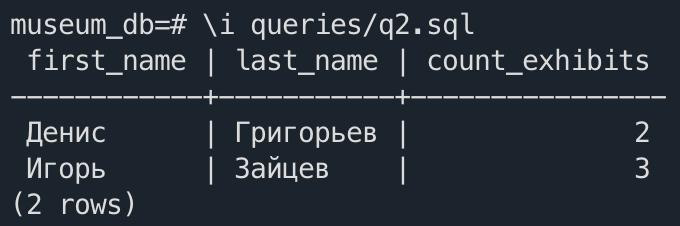
\includegraphics[width=\textwidth,height=3cm,keepaspectratio]{pic/q2.jpg}
    \caption{Результат выполнения запроса 2 (выведены первые 20 строк)}
    \label{fig:q2-result}
\end{figure}

План выполнения запроса 2 представлен на Рис.\ref{fig:q2-explain}. \par

\begin{figure}[H]
    \centering
    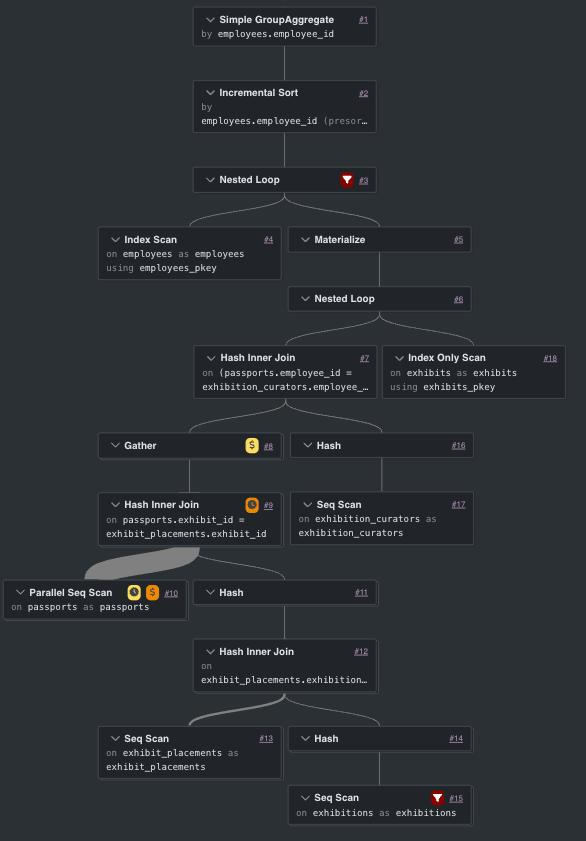
\includegraphics[width=\textwidth,height=0.9\textheight,keepaspectratio]{pic/exp2.jpg}
    \caption{План выполнения запроса 2}
    \label{fig:q2-explain}
\end{figure}

План сначала отбирает заданную выставку, затем соединяет ее с кураторами, сотрудниками, паспортами, экспонатами и размещениями. После соединений выполняется группировка по сотруднику и подсчет различных экспонатов, относящихся к выбранной выставке. \par

\subsection{Запрос 3}

Для каждой выставки посчитать число экспонатов и технических паспортов. Текст запроса представлен в Листинге~\ref{lst:q3}. \par

\lstinputlisting[language=SQL, caption={Запрос 3}, label={lst:q3}, basicstyle=\ttfamily\footnotesize]{../../../queries/q3.sql}

Реляционная формула запроса:
\[
\begin{gathered}
R_3 = 
\gamma_{\substack{\text{exhibition\_id}, \text{exhibition\_name}; \\ \text{COUNT}(\text{distinct } \text{exhibit\_id}), \\ \text{COUNT}(\text{distinct } \text{passport\_id})}}
\left(
\begin{gathered}
\text{exhibitions}
\bowtie(left)_{\text{exhibition\_id}} \\
\text{exhibit\_placements}
\bowtie(left)_{\text{exhibit\_id}} \\
\text{passports}
\end{gathered}
\right), \\
\text{где } \bowtie \text{ --- это natural join}
\end{gathered}
\]

Результат выполнения запроса 3 (выведены первые 20 строк) представлен на Рис.\ref{fig:q3-result}. \par

\begin{figure}[H]
    \centering
    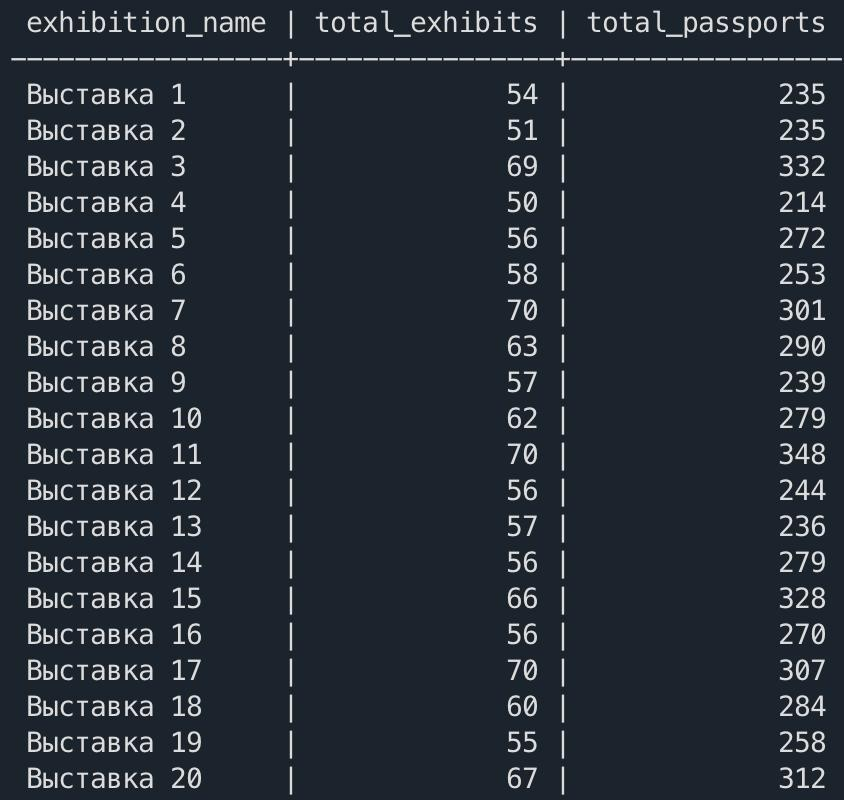
\includegraphics[width=\textwidth,height=8cm,keepaspectratio]{pic/q3.jpg}
    \caption{Результат выполнения запроса 3 (выведены первые 20 строк)}
    \label{fig:q3-result}
\end{figure}

Двумерная гистограмма, построенная по результатам запроса 3, представлена на Рис.\ref{fig:q3-histogram}. \par

\begin{figure}[H]
    \centering
    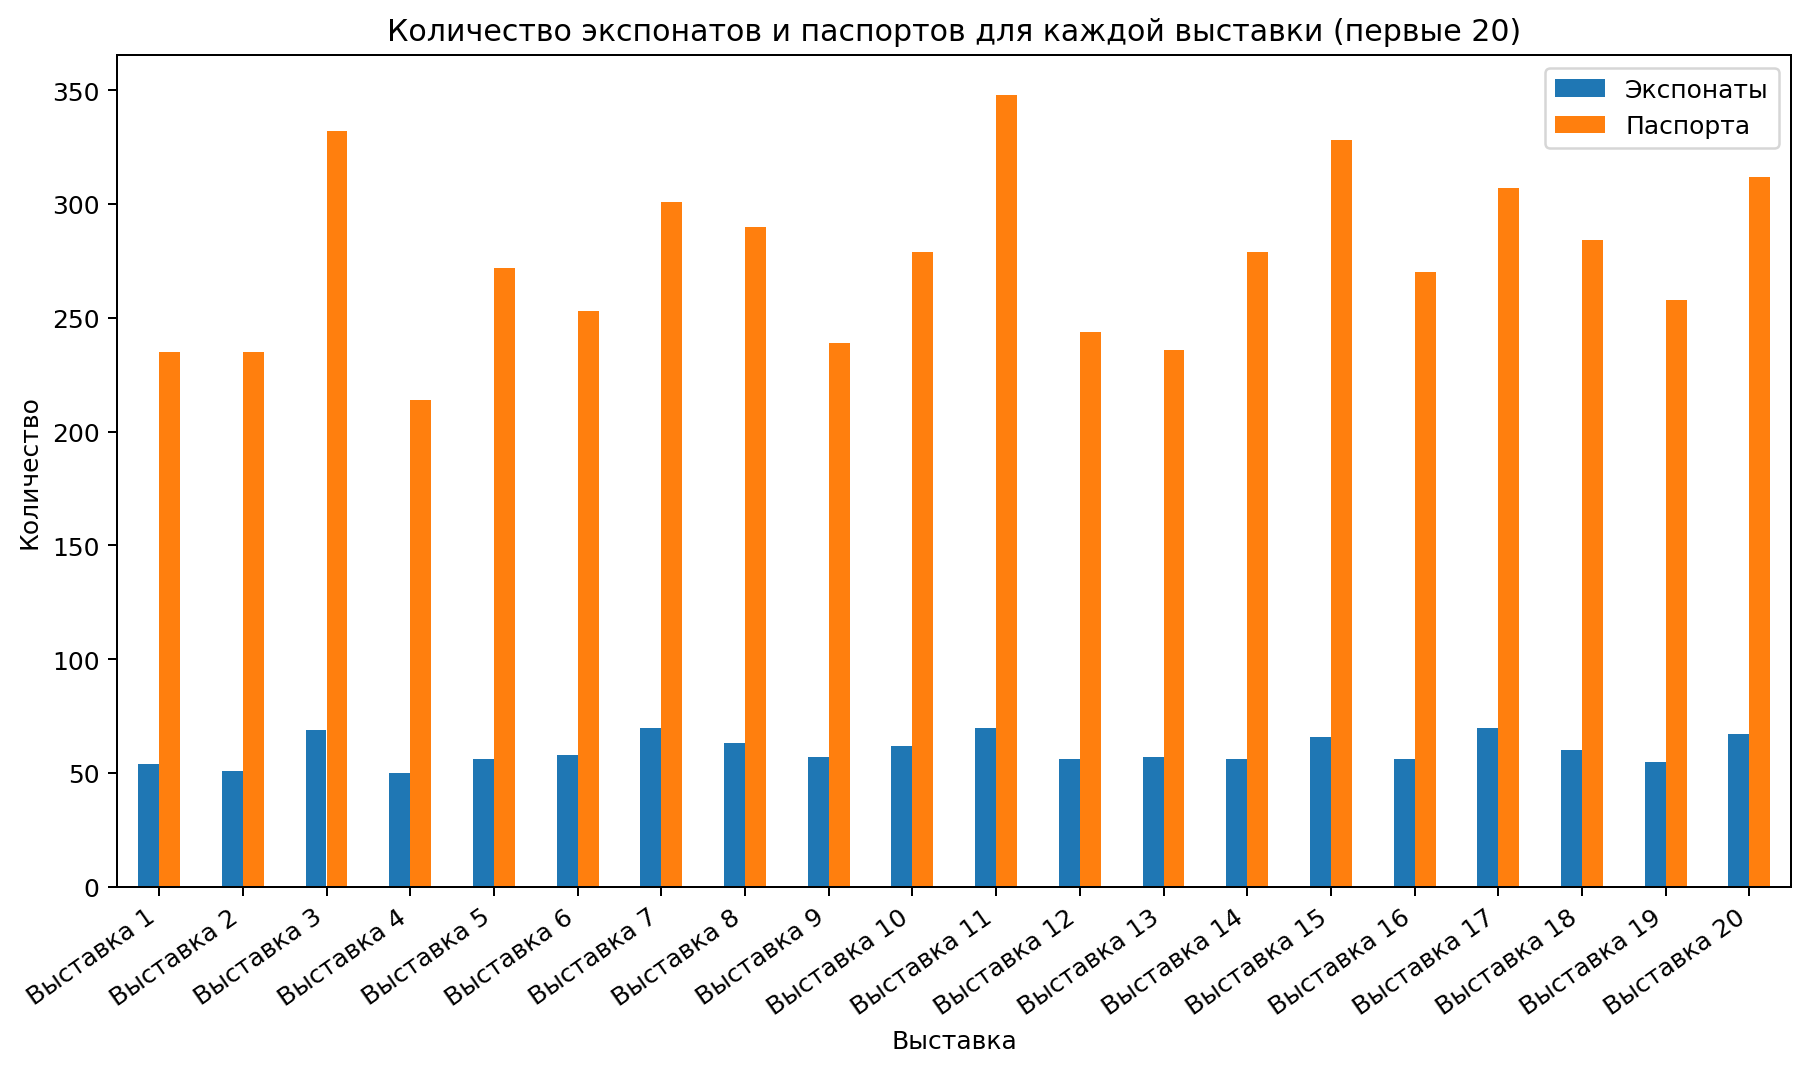
\includegraphics[width=\textwidth,height=14cm, keepaspectratio]{pic/q3_2d_histogram.png}
    \caption{Двумерная гистограмма по результатам запроса 3}
    \label{fig:q3-histogram}
\end{figure}

План выполнения запроса 3 представлен на Рис.\ref{fig:q3-explain}. \par

\begin{figure}[H]
    \centering
    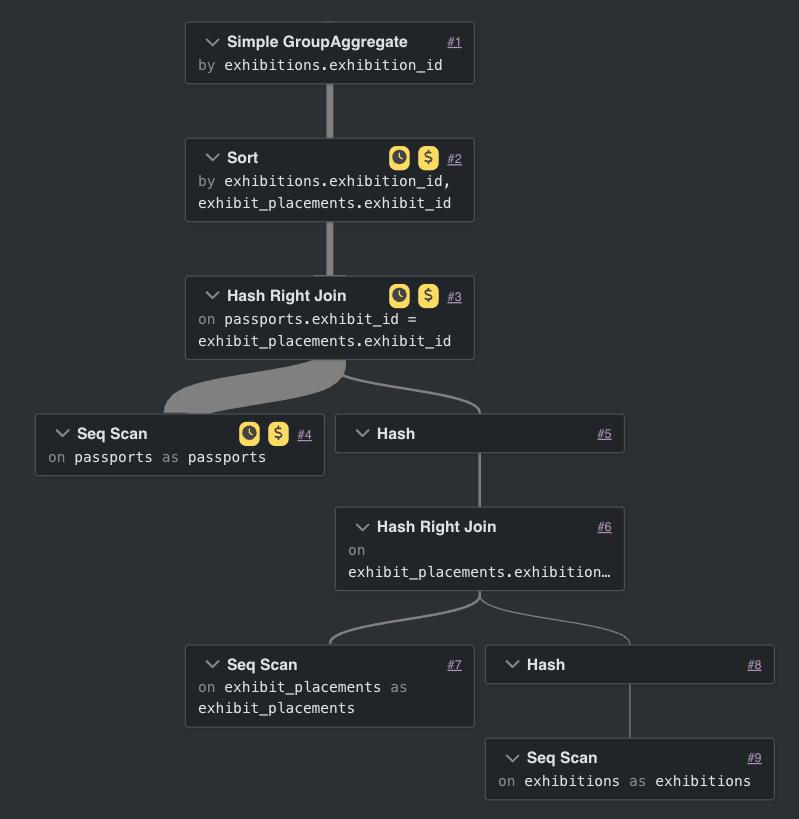
\includegraphics[width=\textwidth,height=12cm,keepaspectratio]{pic/exp3.jpg}
    \caption{План выполнения запроса 3}
    \label{fig:q3-explain}
\end{figure}

План использует внешние соединения, потому что выставка может не иметь размещенных экспонатов, а экспонат может не иметь паспорта. После соединения таблиц выполняется группировка по выставке и два агрегатных подсчета: число различных экспонатов и число различных паспортов. \par

\subsection{Запрос 4.1}

Найти выставочные пространства с максимальным числом выставленных экспонатов. Текст запроса представлен в Листинге~\ref{lst:q41}. \par

\lstinputlisting[language=SQL, caption={Запрос 4.1}, label={lst:q41}, basicstyle=\ttfamily\footnotesize]{../../../queries/q41.sql}

Реляционная формула запроса:
\[
\begin{gathered}
T = 
\gamma_{\substack{\text{exhibition\_space\_id}, \text{room\_type\_name}; \\ \text{COUNT}(\text{exhibit\_id})}}
\left(
\begin{gathered}
\text{exhibition\_spaces} 
\bowtie_{\text{room\_type\_id}} \\
\text{room\_type} 
\bowtie_{\text{exhibition\_space\_id}} \\
\text{display\_places} 
\bowtie_{\text{display\_place\_id}} \\
\text{exhibit\_placements}
\end{gathered}
\right), \\
R_{4.1} = 
\sigma_{\substack{\text{COUNT}(\text{exhibit\_id}) \ = \\ \text{MAX}(\text{COUNT}(\text{exhibit\_id}))}}(T), \\
\text{где } \bowtie \text{ --- это natural join}
\end{gathered}
\]

Результат выполнения запроса 4.1 (выведены первые 20 строк) представлен на Рис.\ref{fig:q41-result}. \par

\begin{figure}[H]
    \centering
    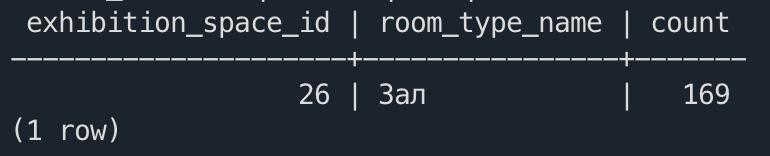
\includegraphics[width=\textwidth,height=2cm,keepaspectratio]{pic/q41.jpg}
    \caption{Результат выполнения запроса 4.1 (выведены первые 20 строк)}
    \label{fig:q41-result}
\end{figure}

План выполнения запроса 4.1 представлен на Рис.\ref{fig:q41-explain}. \par

\begin{figure}[H]
    \centering
    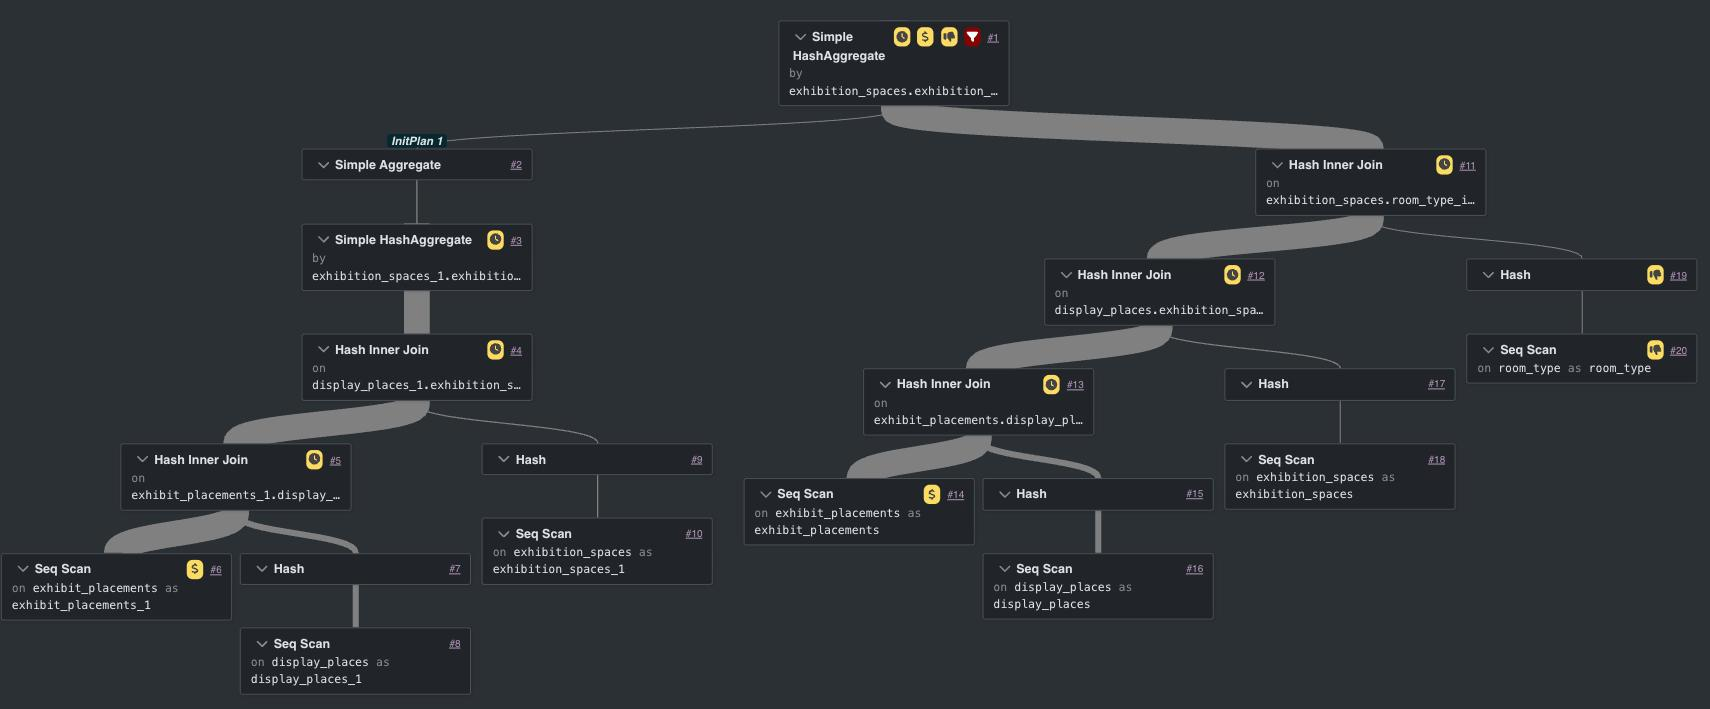
\includegraphics[width=\textwidth,height=0.9\textheight,keepaspectratio]{pic/exp4.1.jpg}
    \caption{План выполнения запроса 4.1}
    \label{fig:q41-explain}
\end{figure}

План строит агрегированную таблицу по выставочным пространствам: соединяет пространства с типами помещений, местами экспонирования и фактами размещения, затем считает число экспонатов. Отдельный подзапрос вычисляет максимальное значение этого счетчика, после чего основной результат фильтруется по равенству максимуму. \par

\subsection{Запрос 4.2}

Найти выставочные пространства с минимальным числом выставленных экспонатов. Текст запроса представлен в Листинге~\ref{lst:q42}. \par

\lstinputlisting[language=SQL, caption={Запрос 4.2}, label={lst:q42}, basicstyle=\ttfamily\footnotesize]{../../../queries/q42.sql}

Реляционная формула запроса:
\[
\begin{gathered}
T = 
\gamma_{\substack{\text{exhibition\_space\_id}, \text{room\_type\_name}; \\ \text{COUNT}(\text{exhibit\_id})}}
\left(
\begin{gathered}
\text{exhibition\_spaces} 
\bowtie_{\text{room\_type\_id}} \\
\text{room\_type} 
\bowtie_{\text{exhibition\_space\_id}} \\
\text{display\_places} 
\bowtie_{\text{display\_place\_id}} \\
\text{exhibit\_placements}
\end{gathered}
\right), \\
R_{4.2} = 
\sigma_{\substack{\text{COUNT}(\text{exhibit\_id}) \ = \\ \text{MIN}(\text{COUNT}(\text{exhibit\_id}))}}(T), \\
\text{где } \bowtie \text{ --- это natural join}
\end{gathered}
\]

Результат выполнения запроса 4.2 (выведены первые 20 строк) представлен на Рис.\ref{fig:q42-result}. \par

\begin{figure}[H]
    \centering
    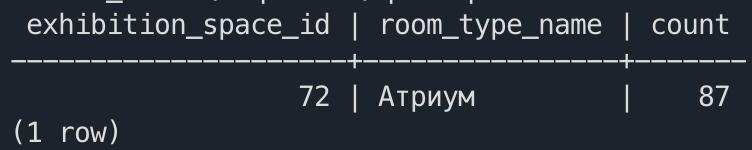
\includegraphics[width=\textwidth,height=2cm,keepaspectratio]{pic/q4.2.jpg}
    \caption{Результат выполнения запроса 4.2 (выведены первые 20 строк)}
    \label{fig:q42-result}
\end{figure}

План выполнения запроса 4.2 представлен на Рис.\ref{fig:q42-explain}. \par

\begin{figure}[H]
    \centering
    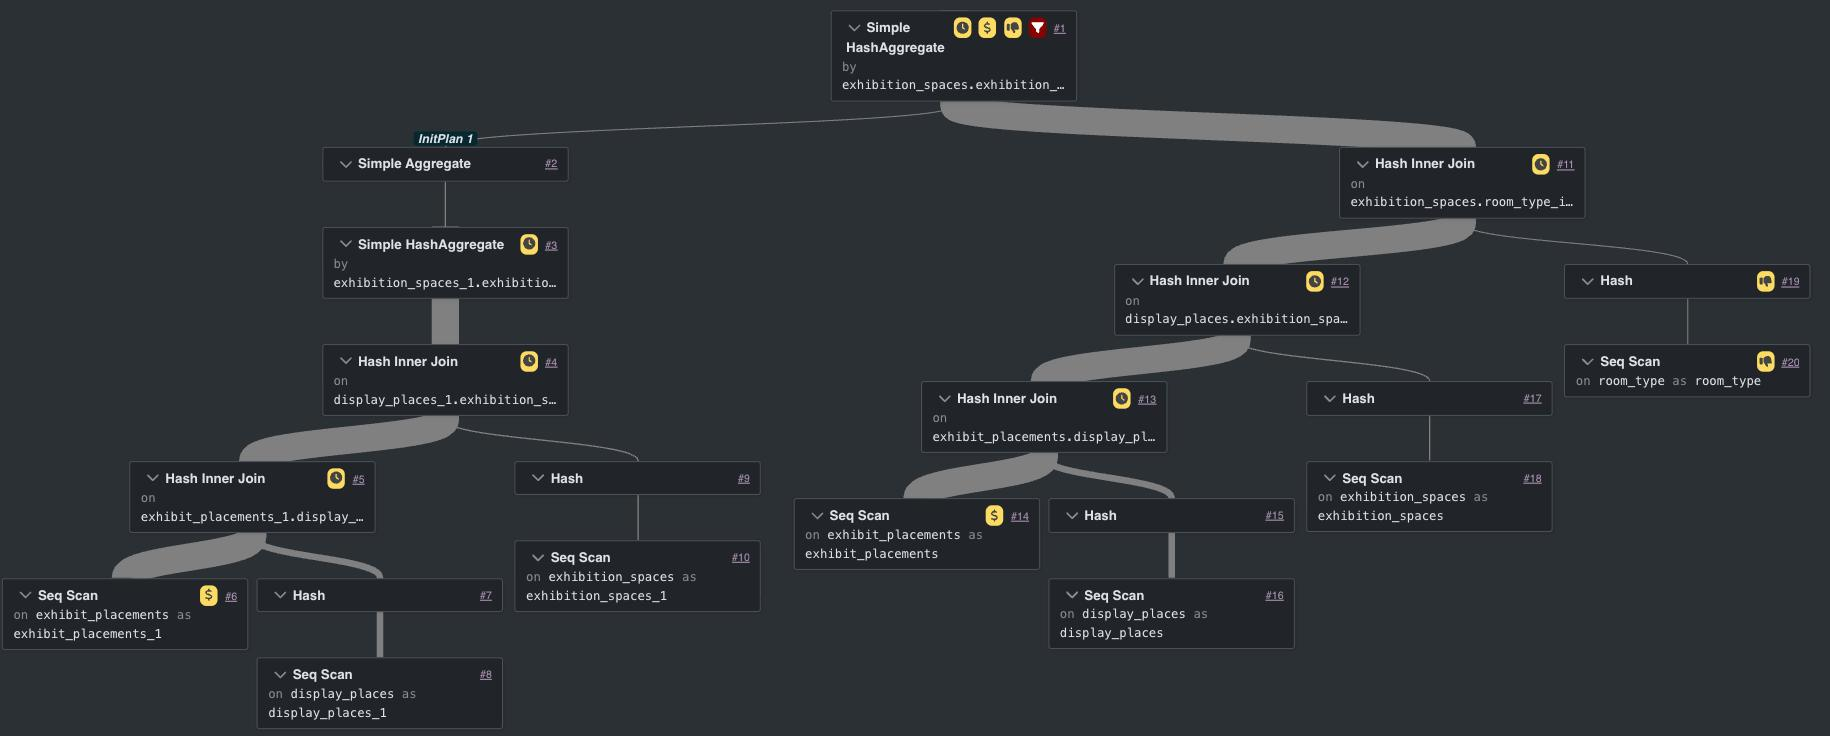
\includegraphics[width=\textwidth,height=0.9\textheight,keepaspectratio]{pic/exp4.2.jpg}
    \caption{План выполнения запроса 4.2}
    \label{fig:q42-explain}
\end{figure}

План аналогичен запросу 4.1: сначала формируется количество размещенных экспонатов по каждому выставочному пространству. Отличие состоит в подзапросе условия HAVING: вместо максимального значения вычисляет минимум, и в итог попадают пространства с минимальным числом экспонатов. \par

\subsection{Запрос 5}

Посчитать число экспонатов с одинаковым числом технических паспортов. Текст запроса представлен в Листинге~\ref{lst:q5}. \par

\lstinputlisting[language=SQL, caption={Запрос 5}, label={lst:q5}, basicstyle=\ttfamily\footnotesize]{../../../queries/q5.sql}

Реляционная формула запроса:
\[
\begin{gathered}
T = 
\gamma_{\substack{\text{exhibit\_id}; \\ \text{COUNT}(\text{passport\_id})}}
\left(
\text{exhibits} \ \bowtie(left)_{\text{exhibit\_id}} \ \text{passports}
\right), \\
R_5 = 
\gamma_{\substack{\text{COUNT}(\text{passport\_id}); \\ \text{COUNT}(\text{exhibit\_id})}}(T), \\
\text{где } \bowtie \text{ --- это natural join}
\end{gathered}
\]

Результат выполнения запроса 5 (выведены первые 20 строк) представлен на Рис.\ref{fig:q5-result}. \par

\begin{figure}[H]
    \centering
    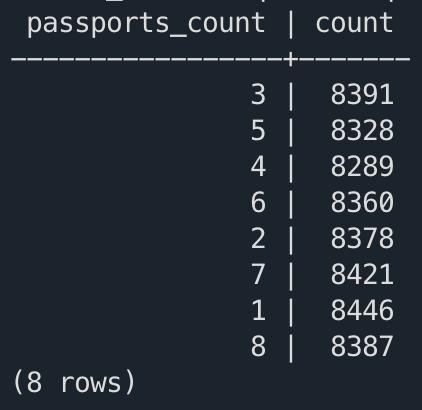
\includegraphics[width=\textwidth,height=7cm,keepaspectratio]{pic/q5.jpg}
    \caption{Результат выполнения запроса 5 (выведены первые 20 строк)}
    \label{fig:q5-result}
\end{figure}

Двумерная гистограмма, построенная по результатам запроса 5, представлена на Рис.\ref{fig:q5-histogram}. \par

\begin{figure}[H]
    \centering
    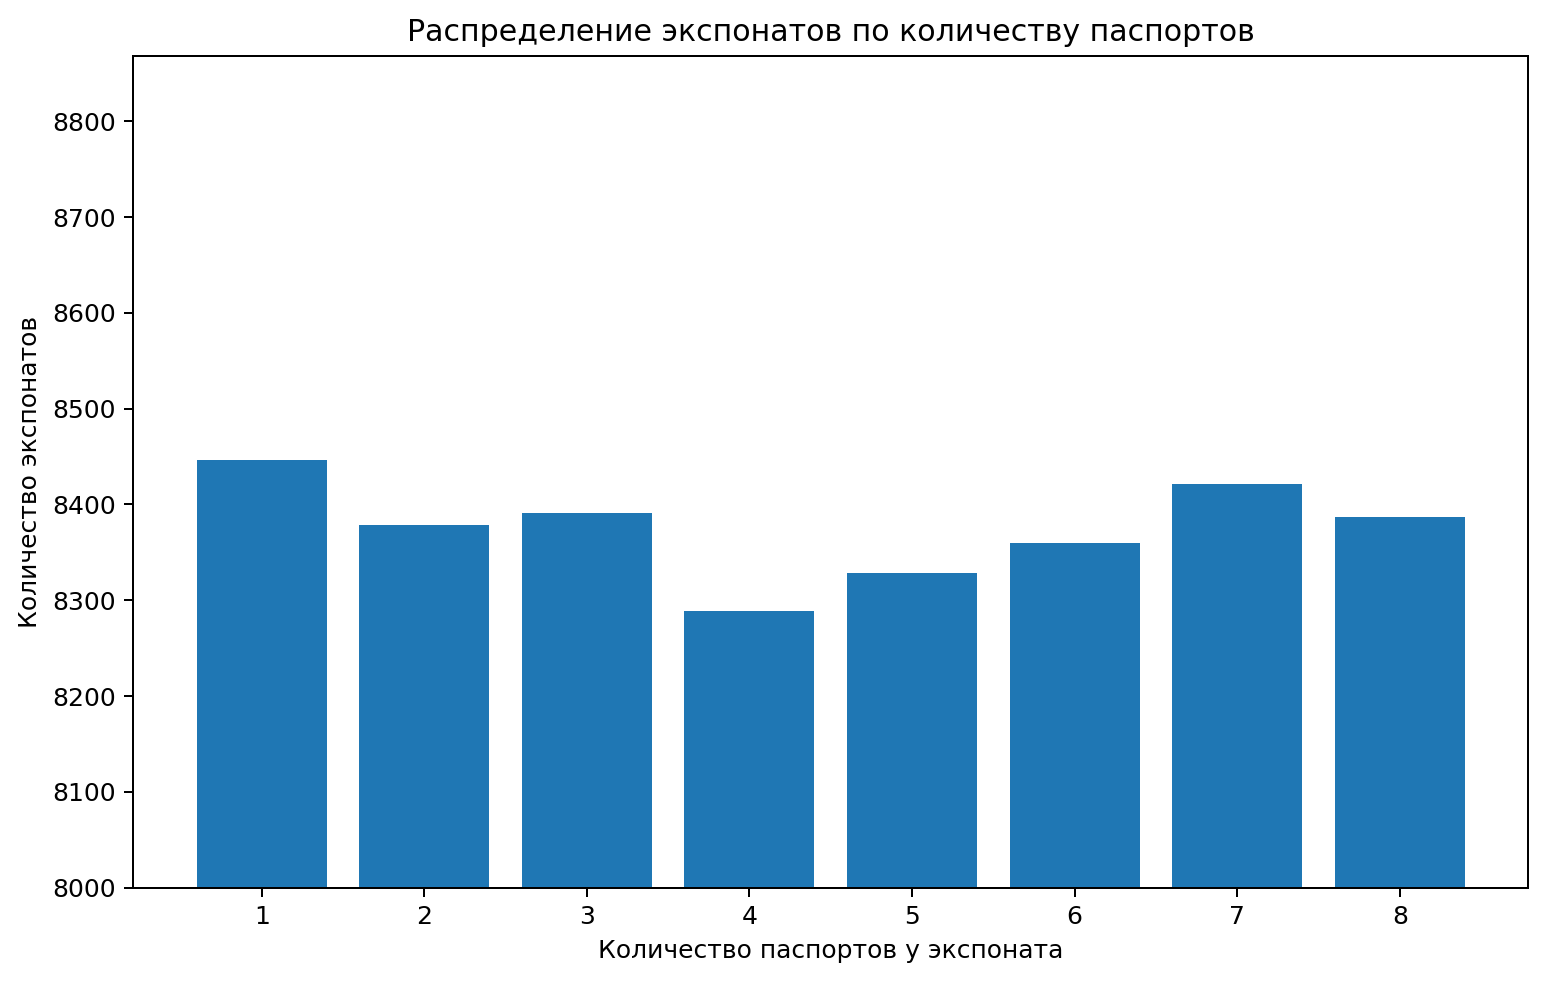
\includegraphics[width=\textwidth,height=0.6\textheight,keepaspectratio]{pic/q5_2d_histogram.png}
    \caption{Двумерная гистограмма по результатам запроса 5}
    \label{fig:q5-histogram}
\end{figure}

План выполнения запроса 5 представлен на Рис.\ref{fig:q5-explain}. \par

\begin{figure}[H]
    \centering
    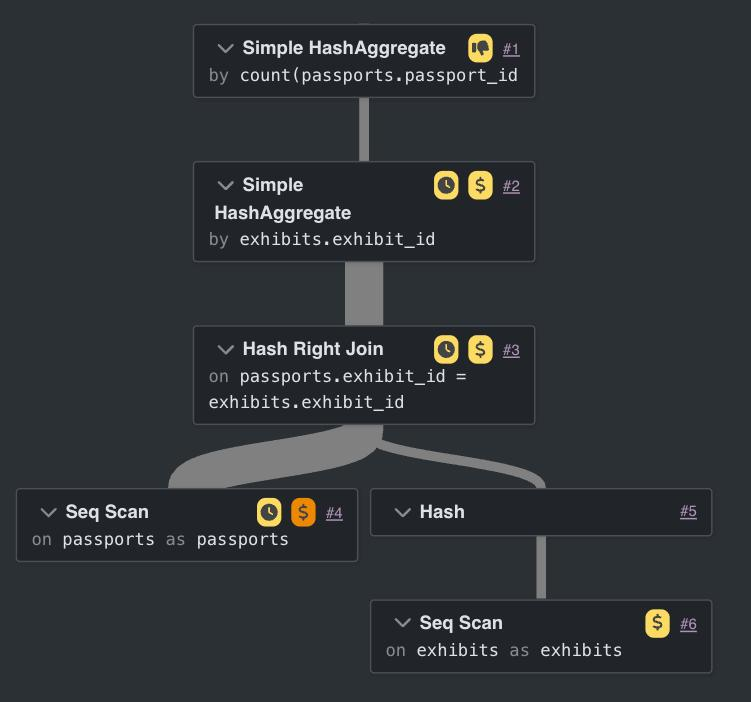
\includegraphics[width=\textwidth,height=0.4\textheight,keepaspectratio]{pic/exp5.jpg}
    \caption{План выполнения запроса 5}
    \label{fig:q5-explain}
\end{figure}

В плане сначала выполняется внешнее соединение экспонатов с паспортами, чтобы учесть в том числе экспонаты без паспортов. Затем подзапрос группирует строки по экспонату и считает паспорта, а внешний запрос группирует уже по полученному числу паспортов и считает количество экспонатов в каждой группе. \par

\subsection{Запрос 6}

Найти выставки, на которых было больше мест экспонирования, чем на выставке А. Текст запроса представлен в Листинге~\ref{lst:q6}. \par

\lstinputlisting[language=SQL, caption={Запрос 6}, label={lst:q6}, basicstyle=\ttfamily\footnotesize]{../../../queries/q6.sql}

Реляционная формула запроса:
\[
\begin{gathered}
T = 
\gamma_{\substack{\text{exhibition\_id}, \text{exhibition\_name}; \\ \text{COUNT}(\text{display\_place\_id})}}
\left(
\begin{gathered}
\text{exhibitions} 
\bowtie_{\text{exhibition\_id}} \\
\text{exhibit\_placements} 
\bowtie_{\text{display\_place\_id}} \\
\text{display\_places}
\end{gathered}
\right), \\
H = 
\gamma_{\text{COUNT}(\text{display\_place\_id})}
\left(
\sigma_{\text{exhibition\_name}=A}
\left(
\text{exhibitions} \ \bowtie_{\text{exhibition\_id}} \ \text{exhibit\_placements}
\right)
\right), \\
R_6 = 
\sigma_{\substack{\text{COUNT}(\text{display\_place\_id}) \ > H}}(T), \\
\text{где } \bowtie \text{ --- это natural join}
\end{gathered}
\]

Результат выполнения запроса 6 (выведены первые 20 строк) представлен на Рис.\ref{fig:q6-result}. \par

\begin{figure}[H]
    \centering
    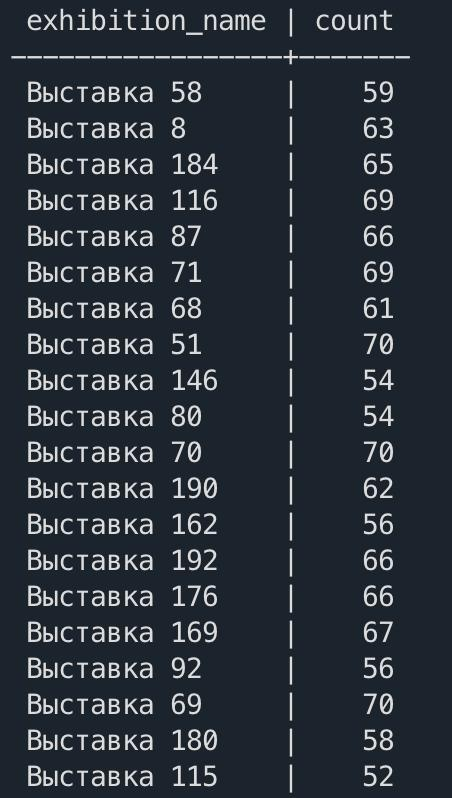
\includegraphics[width=\textwidth,height=10cm,keepaspectratio]{pic/q6.jpg}
    \caption{Результат выполнения запроса 6 (выведены первые 20 строк)}
    \label{fig:q6-result}
\end{figure}

План выполнения запроса 6 представлен на Рис.\ref{fig:q6-explain}. \par

\begin{figure}[H]
    \centering
    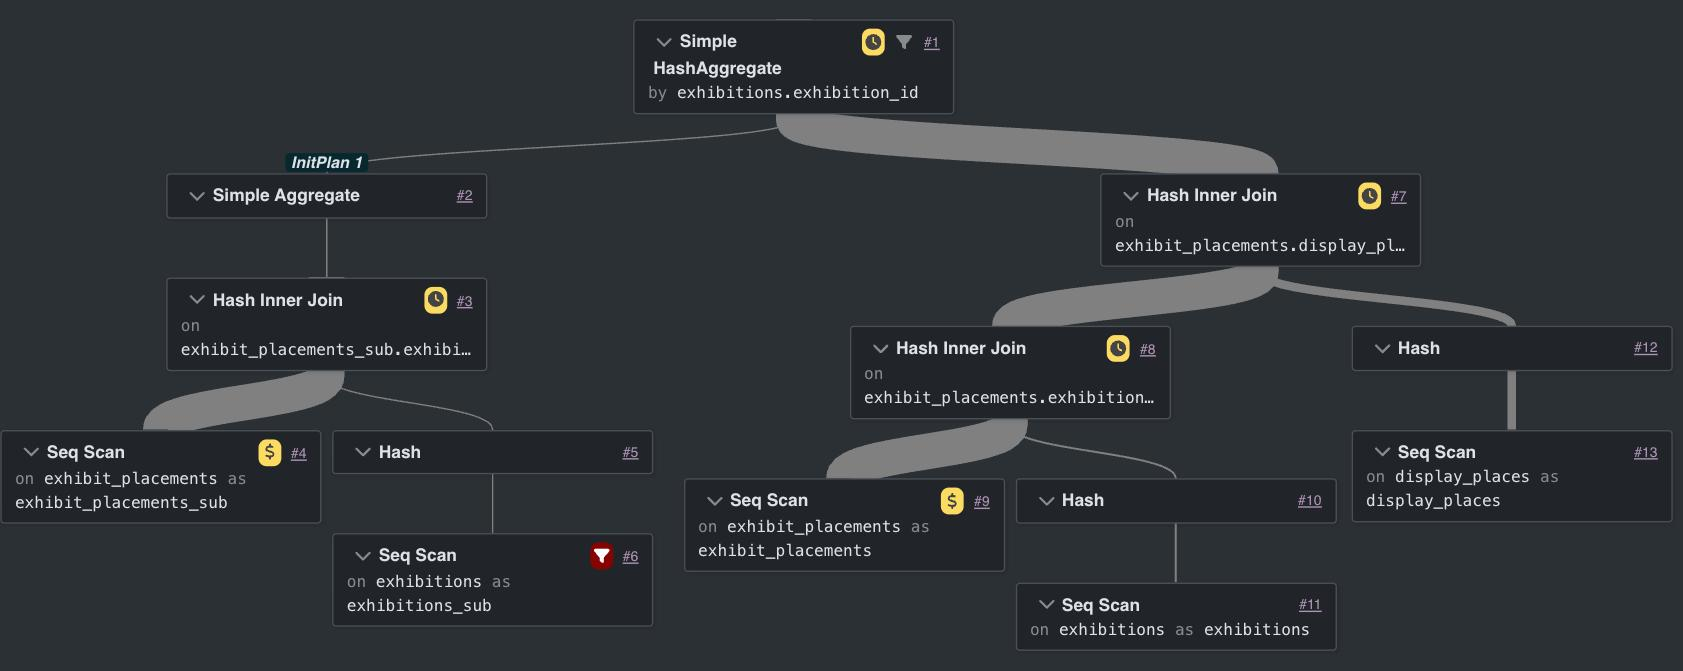
\includegraphics[width=\textwidth,height=0.75\textheight,keepaspectratio]{pic/exp6.jpg}
    \caption{План выполнения запроса 6}
    \label{fig:q6-explain}
\end{figure}

План состоит из двух агрегирующих частей. Подзапрос считает количество мест экспонирования для заданной выставки, а основной запрос считает количество мест для каждой выставки. После группировки применяется условие HAVING, оставляющее только выставки, где количество мест больше значения из подзапроса. \par

\subsection{Запрос 7}

Найти сотрудников, которые ни разу не выставляли ни на одной выставке в качестве кураторов экспонат А. Текст запроса представлен в Листинге~\ref{lst:q7}. \par

\lstinputlisting[language=SQL, caption={Запрос 7}, label={lst:q7}, basicstyle=\ttfamily\footnotesize]{../../../queries/q72.sql}

Реляционная формула запроса:
\[
\begin{gathered}
R_7 = 
\pi_{\text{first\_name}, \text{last\_name}}
\left(
\begin{gathered}
\left(
\text{employees} \ \bowtie_{\text{employee\_id}} \ \text{exhibition\_curators}
\right) - \\ - 
\pi_{\substack{\text{employee\_id}, \\ \text{first\_name}, \\ \text{last\_name}}}
\left(
\sigma_{\text{exhibit\_name}=A}
\left(
\begin{gathered}
\text{employees} \\
\bowtie_{\text{employee\_id}} \\
\text{exhibition\_curators} \\
\bowtie_{\text{exhibition\_id}} \\
\text{exhibitions} \\
\bowtie_{\text{exhibition\_id}} \\
\text{exhibit\_placements} \\
\bowtie_{\text{exhibit\_id}} \\
\text{exhibits}
\end{gathered}
\right)
\right)
\end{gathered}
\right), \\
\text{где } \bowtie \text{ --- это natural join}
\end{gathered}
\]

Результат выполнения запроса 7 (выведены первые 20 строк) представлен на Рис.\ref{fig:q7-result}. \par

\begin{figure}[H]
    \centering
    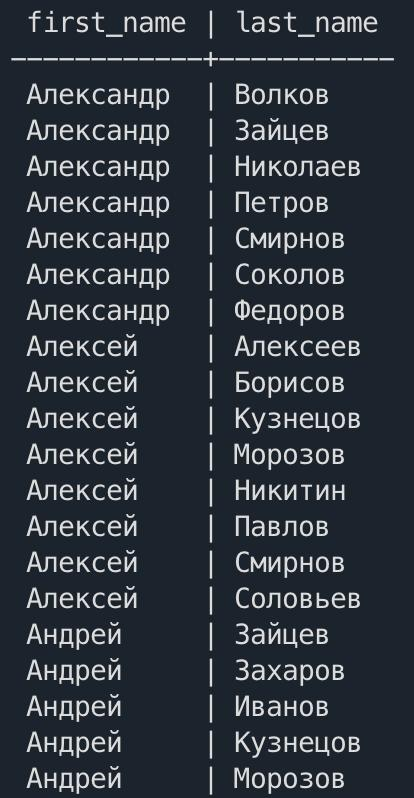
\includegraphics[width=\textwidth,height=8cm,keepaspectratio]{pic/q7.jpg}
    \caption{Результат выполнения запроса 7 (выведены первые 20 строк)}
    \label{fig:q7-result}
\end{figure}

План выполнения запроса 7 представлен на Рис.\ref{fig:q7-explain}. \par

\begin{figure}[H]
    \centering
    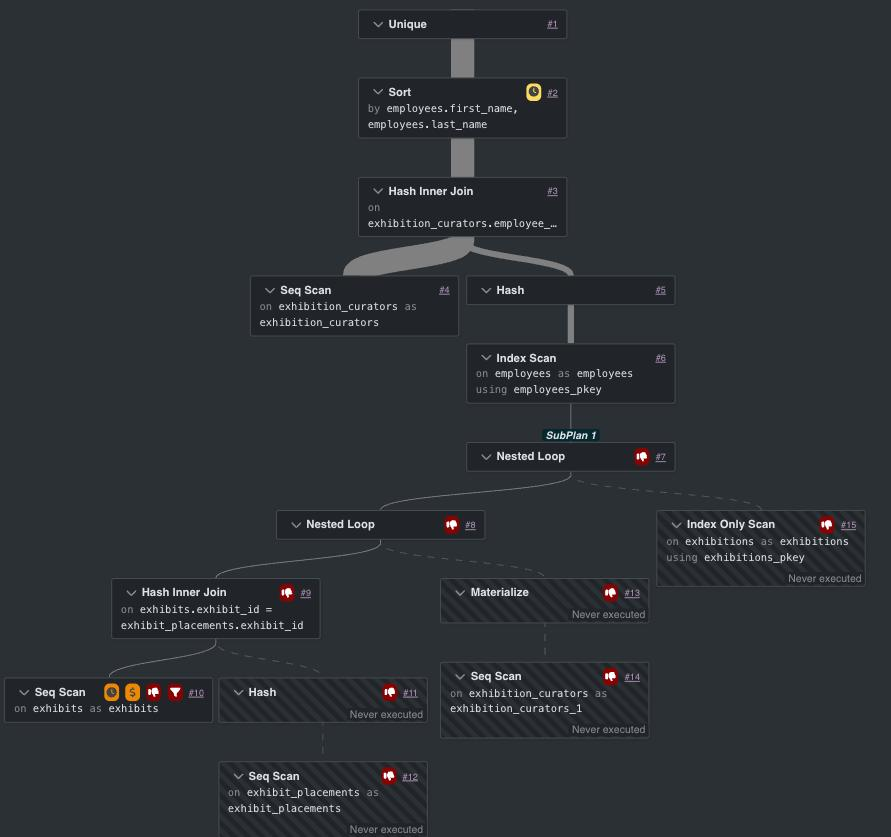
\includegraphics[width=\textwidth,height=0.75\textheight,keepaspectratio]{pic/exp7.jpg}
    \caption{План выполнения запроса 7}
    \label{fig:q7-explain}
\end{figure}

План получает множество сотрудников, которые вообще выступали кураторами, а затем исключает из него сотрудников из подзапроса. Подзапрос находит кураторов выставок, где размещался заданный экспонат. Операция DISTINCT удаляет повторения сотрудников в итоговом результате. \par

\subsection{Запрос 8}

Для каждой выставки и каждого статуса экспоната посчитать число экспонатов. Текст запроса представлен в Листинге~\ref{lst:q8}. \par

\lstinputlisting[language=SQL, caption={Запрос 8}, label={lst:q8}, basicstyle=\ttfamily\footnotesize]{../../../queries/q8.sql}

Реляционная формула запроса:
\[
\begin{gathered}
R_8 = 
\gamma_{\substack{\text{exhibition\_name}, \text{exhibit\_status\_name}; \\ \text{COUNT}(\text{real\_status\_id})}}
\left(
\begin{gathered}
\left(
\text{exhibitions} \times \text{exhibit\_status}
\right) 
\bowtie(left)_{\text{exhibition\_id}} \\
\text{exhibit\_placements} 
\bowtie(left)_{\text{exhibit\_id}} \\
\text{exhibits} 
\bowtie(left)_{\substack{\text{exhibit\_status\_id} \\ \text{exhibit\_status\_name}}} \\
\text{real\_status}
\end{gathered}
\right), \\
\text{где } \bowtie \text{ --- это natural join}
\end{gathered}
\]

Результат выполнения запроса 8 (выведены первые 20 строк) представлен на Рис.\ref{fig:q8-result}. \par

\begin{figure}[H]
    \centering
    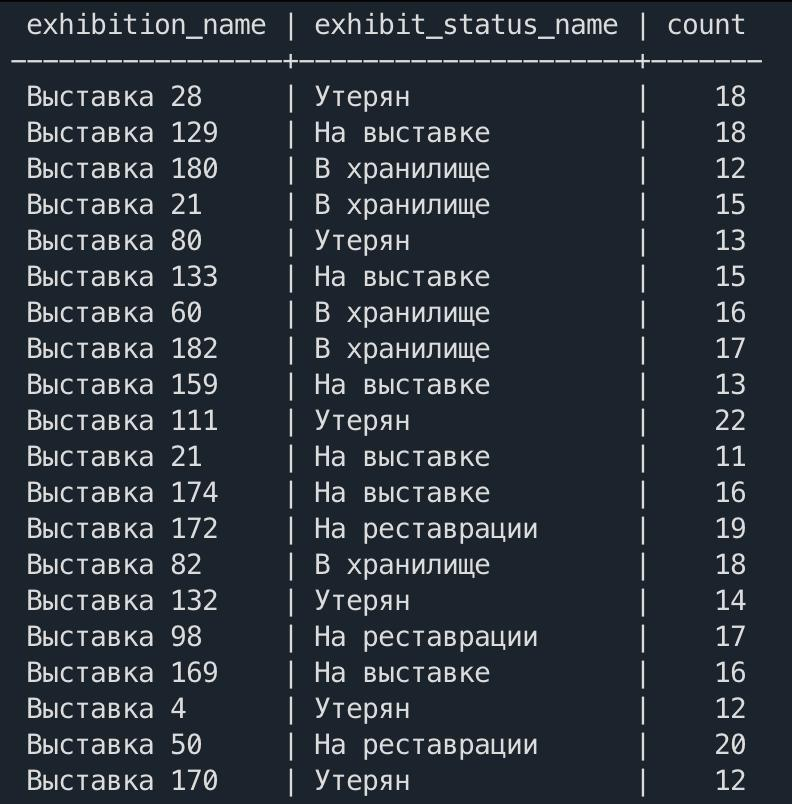
\includegraphics[width=\textwidth,height=0.8\textheight,keepaspectratio]{pic/q8.jpg}
    \caption{Результат выполнения запроса 8 (выведены первые 20 строк)}
    \label{fig:q8-result}
\end{figure}

Трехмерная гистограмма, построенная по результатам запроса 8, представлена на Рис.\ref{fig:q8-histogram}. \par

\begin{figure}[H]
    \centering
    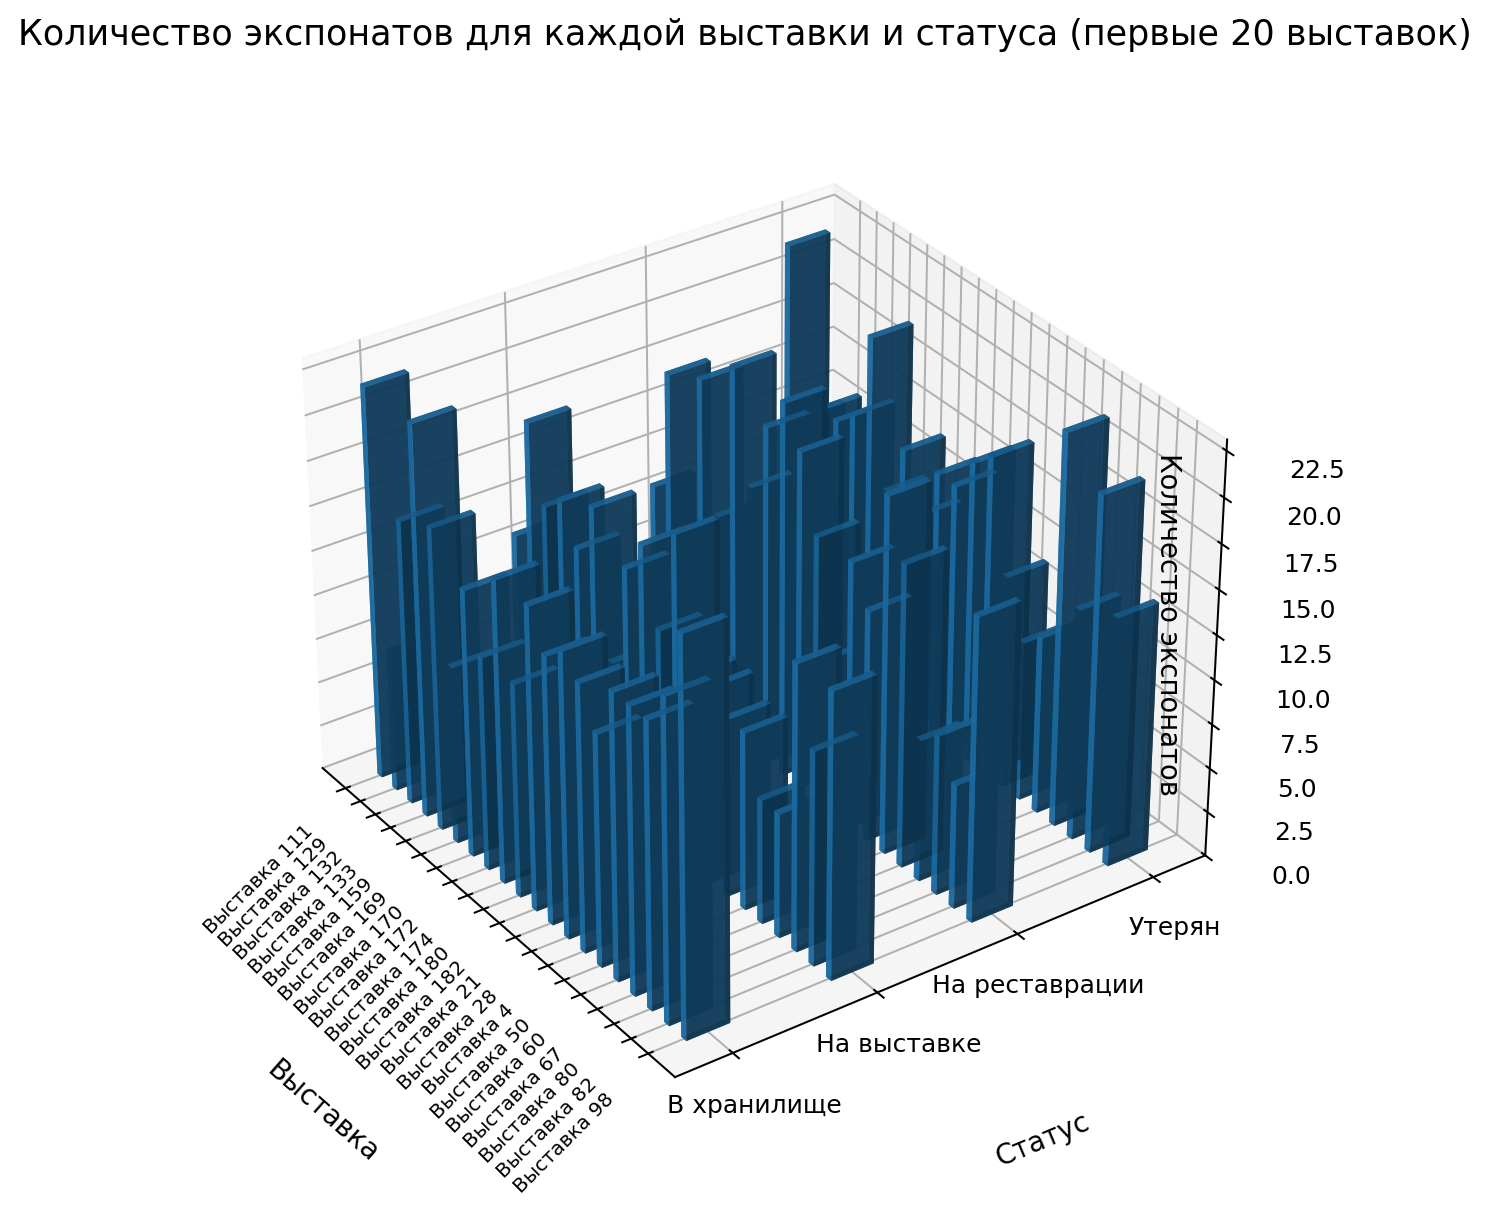
\includegraphics[width=\textwidth,height=0.6\textheight,keepaspectratio]{pic/q8_3d_histogram.png}
    \caption{Трехмерная гистограмма по результатам запроса 8}
    \label{fig:q8-histogram}
\end{figure}

План выполнения запроса 8 представлен на Рис.\ref{fig:q8-explain}. \par

\begin{figure}[H]
    \centering
    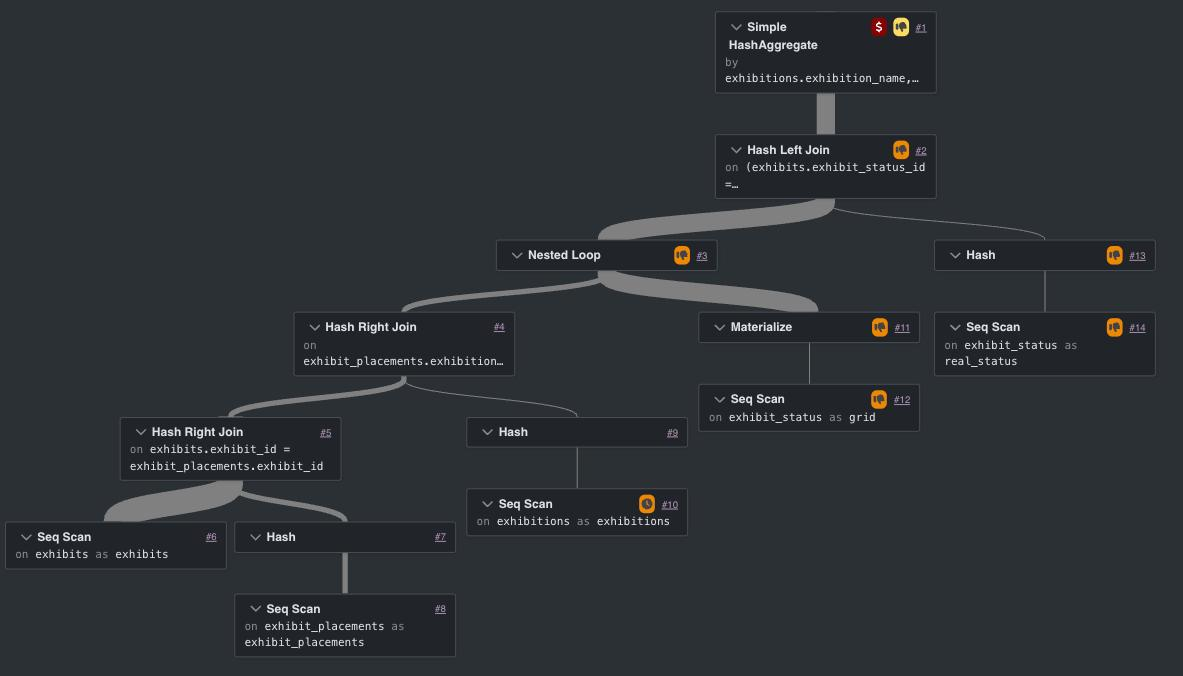
\includegraphics[width=\textwidth,height=0.75\textheight,keepaspectratio]{pic/exp8.jpg}
    \caption{План выполнения запроса 8}
    \label{fig:q8-explain}
\end{figure}

В плане сначала формируется сетка всех пар ``выставка--статус'' с помощью декартова произведения. Затем через внешние соединения добавляются размещения и экспонаты. Последнее соединение со статусом выполнено с дополнительным условием совпадения со строкой сетки, поэтому агрегирование возвращает количество экспонатов для каждой пары выставки и статуса, включая нулевые комбинации. \par

\subsection{Запрос 9}

Для каждого технического паспорта, который составлял сотрудник А, поменять состояние экспоната в паспорте с Б на В. Текст запроса представлен в Листинге~\ref{lst:q9}. \par

\lstinputlisting[language=SQL, caption={Запрос 9}, label={lst:q9}, basicstyle=\ttfamily\footnotesize]{../../../queries/q9.sql}

Реляционная формула запроса:
\[
\begin{gathered}
\text{UPDATE}_{\text{condition\_id} \leftarrow newid} 
\left( 
\text{passports}, 
\right. 
\left.
\sigma_{\text{passport\_id} \in \pi_{\text{passport\_id}}(S)}(\text{passports}) 
\right) \\
 \quad S = 
\sigma_{\substack{\text{last\_name} = A \ \land \\ \text{exhibit\_conditions\_name} = B}}
\left(
\begin{gathered}
\text{passports} 
\bowtie \text{employees} 
\bowtie \text{exhibit\_conditions}
\end{gathered}
\right) \\
newid = 
\pi_{\text{exhibit\_conditions\_id}}
\left(
\sigma_{\text{exhibit\_conditions\_name} = C}(\text{exhibit\_conditions})
\right), \\
\text{где } \bowtie \text{ --- это natural join}
\end{gathered}
\]

Результат выполнения запроса 9 (выведены первые 20 строк) представлен на Рис.\ref{fig:q9-result}. \par

\begin{figure}[H]
    \centering
    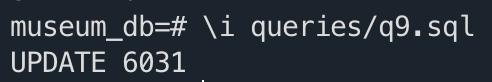
\includegraphics[width=\textwidth,height=2cm,keepaspectratio]{pic/q9.jpg}
    \caption{Результат выполнения запроса 9 (выведены первые 20 строк)}
    \label{fig:q9-result}
\end{figure}

План выполнения запроса 9 представлен на Рис.\ref{fig:q9-explain}. \par

\begin{figure}[H]
    \centering
    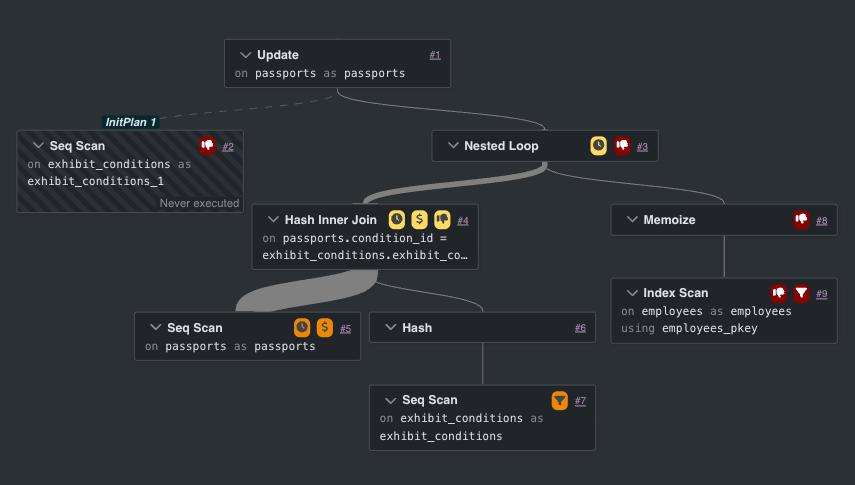
\includegraphics[width=\textwidth,height=0.75\textheight,keepaspectratio]{pic/exp9.jpg}
    \caption{План выполнения запроса 9}
    \label{fig:q9-explain}
\end{figure}

План обновления отбирает паспорта, связанные с сотрудником с заданной фамилией и текущим состоянием экспоната. Подзапрос предварительно получает идентификатор нового состояния по его названию. После отбора строк выполняется операция UPDATE, изменяющая поле \texttt{condition\_id} у найденных технических паспортов. \par

\newpage

%Заключение
\noindent
{\Large \textbf{\section*{Заключение}}} \par
\addcontentsline{toc}{section}{Заключение} \par

В ходе выполнения курсовой работы была выбрана предметная область «Организация выставочной деятельности музея». 
При ее анализе было задействовано 4 источника, указанные в списке использованных источников.
По результатам данного анализа были сформированы 3 цели функционирования базы данных:
ведение централизованного реестра музейных предметов, ведение реестра проводимых в музее выставок, хранение планов размещения выставок в залах музея.
Также было выделено 4 роли и 10 сущностей. На основании выделенных сущностей была построена ER-диаграмма в нотации Чена и схема связи объектов при помощи онлайн-ресурса draw.io.

На этапе проектирования было выделено 20 таблиц. Для атрибутов были выбраны типы SERIAL, INT, VARCHAR, DECIMAL, при этом выбор каждого типа был обоснован, опираясь на примеры и источники. 
Далее были построены схемы базы данных на русском и английском языках, а также схема заполнения уровней БД в draw.io.

На этапе программирования работа велась на ноутбуке Macbook M4 pro с 16гб оперативной памяти. В качестве IDE использовалась Visual Studio Code, для работы с БД использовалось СУБД PostgreSQL.
Далее при помощи SQL-запросов было создано 20 таблиц, их заполнение было реализовано при помощи языка Python, всего в таблицах 2 646 202 записей. После этого было реализовано 9 запросов на языке SQL.
Для каждого запроса была построена реляционная формула и план выполнения.
Для результатов запросов №3 и №5 дополнительно были построены 2-d гистограммы, а для запроса №8 - 3-d гистограмма.


\newpage

%Список литературы
\addcontentsline{toc}{section}{Список использованных источников} \par

\renewcommand{\refname}{Список использованных источников}
\begin{thebibliography}{}

    \bibitem{site:sources1} Литературно-мемориальный музей Ф.М.Достоевского [Электронный ресурс]. URL: \href{https://dostoevsky.kz/otdely-muzeya}{https://dostoevsky.kz/otdely-muzeya} (Дата обращения: 09.02.2026)
    
    \bibitem{site:sources2} Ханымейский Историко-краеведческий музей [Электронный ресурс]. \\ URL: \href{https://hikm.ru/fond.html}{https://hikm.ru/fond} (Дата обращения: 09.02.2026)

    \bibitem{site:sources3} Электронные ресурсы томского государственного педагогического университета [Электронный ресурс]. URL: \href{https://koi.tspu.ru/koi_books/galkina/otcm.htm}{https://koi.tspu.ru/koi\_books/galkina/otcm} (Дата обращения: 16.02.2026)

    \bibitem{site:sources4} Челябинский государственный музей изобразительных искусств [Электронный ресурс]. URL: \href{https://chelmusart.ru/node/19415}{https://chelmusart.ru/node/19415} (Дата обращения: 16.02.2026)

    \bibitem{site:sources5} Приказ ФНС России от 18.12.2012 N ММВ-7-11/973@ (ред. от 28.10.2022) <<Об утверждении формы и формата представления сведений о воздушных судах и об их владельцах, порядка заполнения формы>> [Электронный ресурс]. URL: \href{https://chelmusart.ru/node/19415}{https://chelmusart.ru/node/19415} (Дата обращения: 25.03.2026)

    \bibitem{site:sources6} Приказ Минкультуры СССР от 17.07.1985 № 290 <<Об утверждении Инструкции по учету и хранению музейных ценностей, находящихся в государственных музеях СССР>> [Электронный ресурс]. URL: \href{https://rags.ru/documents/dop_documents/20/gost_57114/0/prika_38610.html}{https://rags.ru/documents/dop\_documents/20/gost\_57114/0/prika\_38610.html} (Дата обращения: 25.03.2026)

    \bibitem{site:sources7} В Сибири нашли улицу с самым длинным названием в России
     [Электронный ресурс]. URL: \href{https://rg.ru/2017/07/15/reg-sibfo/v-sibiri-nashli-ulicu-s-samym-dlinnym-nazvaniem-v-rossii.html}{https://rg.ru/2017/07/15/reg-sibfo/v-sibiri-nashli-ulicu-s-samym-dlinnym-nazvaniem-v-rossii.html} (Дата обращения: 25.03.2026)

    \bibitem{site:explain} PostgreSQL execution plan visualizer
     [Электронный ресурс]. URL: \href{https://explain.dalibo.com/}{https://explain.dalibo.com/} (Дата обращения: 20.05.2026)
    %\bibitem{kniga1} Новиков Ф.А. Дискретная математика для программистов: Учебник для вузов. 3-е издание. СПб.: Питер, 2009. 384с.

    %\bibitem{kniga1} Кук Д., Бейз Г. Компьютерная математика / Пер. с англ. Г. М. Кобелькова. М.: Наука, Главная редакция физико-математической литературы, 1990. 385с.

    %\bibitem{kniga2} Павловская Т. А., Щупак Ю. А. C++ Объектно-ориентированное программирование: Практикум. СПб.: Питер, 2006. 266 с.

\end{thebibliography}
\newpage

%Приложение
%Приложение А
\noindent
{\Large \textbf{\section*{Приложение}}} \par
\addcontentsline{toc}{section}{Приложение} \par
\noindent
{\Large \textbf{\subsection*{Приложение A Исходный код создания таблиц БД}}} \par
\addcontentsline{toc}{subsection}{Приложение A Исходный код создания таблиц БД} \par

\begin{lstlisting}[caption=sqrt.c, numbers=left, breaklines=true, basicstyle=\normalsize]
-- Level 1

CREATE TABLE IF NOT EXISTS exhibition_status(
    exhibition_status_id SERIAL PRIMARY KEY NOT NULL, 
    exhibition_status_name VARCHAR(11) NOT NULL
);

CREATE TABLE IF NOT EXISTS exhibition_type(
    exhibition_type_id SERIAL PRIMARY KEY NOT NULL, 
    exhibition_type_name VARCHAR(15) NOT NULL
);

CREATE TABLE IF NOT EXISTS exhibition_subject(
    exhibition_subject_id SERIAL PRIMARY KEY NOT NULL, 
    exhibition_subject_name VARCHAR(25) NOT NULL
);

CREATE TABLE IF NOT EXISTS exhibit_status(
    exhibit_status_id SERIAL PRIMARY KEY NOT NULL, 
    exhibit_status_name VARCHAR(25) NOT NULL
);

CREATE TABLE IF NOT EXISTS materials(
    material_id SERIAL PRIMARY KEY NOT NULL, 
    material_name VARCHAR(25) NOT NULL
);

CREATE TABLE IF NOT EXISTS exhibit_conditions(
    exhibit_conditions_id SERIAL PRIMARY KEY NOT NULL, 
    exhibit_conditions_name VARCHAR(18) NOT NULL
);

CREATE TABLE IF NOT EXISTS epochs(
    epoch_id SERIAL PRIMARY KEY NOT NULL, 
    epoch_name VARCHAR(30) NOT NULL
);

CREATE TABLE IF NOT EXISTS temp_categories(
    temp_category_id SERIAL PRIMARY KEY NOT NULL, 
    temp_category_name VARCHAR(9) NOT NULL,
    min_value DECIMAL(4,2),
    max_value DECIMAL(4,2)
);

CREATE TABLE IF NOT EXISTS humidity_categories(
    humidity_category_id SERIAL PRIMARY KEY NOT NULL, 
    humidity_category_name VARCHAR(10) NOT NULL,
    min_value DECIMAL(5,2),
    max_value DECIMAL(5,2)
);

CREATE TABLE IF NOT EXISTS lighting_categories(
    lighting_category_id SERIAL PRIMARY KEY NOT NULL, 
    lighting_category_name VARCHAR(7) NOT NULL,
    min_value DECIMAL(7,2),
    max_value DECIMAL(7,2)
);

CREATE TABLE IF NOT EXISTS room_type(
    room_type_id SERIAL PRIMARY KEY NOT NULL, 
    room_type_name VARCHAR(132) NOT NULL
);

CREATE TABLE IF NOT EXISTS employees(
    employee_id SERIAL PRIMARY KEY NOT NULL, 
    first_name VARCHAR(60) NOT NULL,
    last_name VARCHAR(60) NOT NULL,
    middle_name VARCHAR(60),
    phone_number VARCHAR(15)
);


-- Level 2

CREATE TABLE IF NOT EXISTS exhibits(
    exhibit_id SERIAL PRIMARY KEY NOT NULL,
    exhibit_status_id INT NOT NULL REFERENCES exhibit_status(exhibit_status_id),
    exhibit_name VARCHAR(200) NOT NULL
);

CREATE TABLE IF NOT EXISTS exhibitions(
    exhibition_id SERIAL PRIMARY KEY NOT NULL,
    exhibition_status_id INT REFERENCES exhibition_status(exhibition_status_id),
    exhibition_type_id INT REFERENCES exhibition_type(exhibition_type_id),
    exhibition_subject_id INT REFERENCES exhibition_subject(exhibition_subject_id),
    exhibition_name VARCHAR(150) NOT NULL
);

CREATE TABLE IF NOT EXISTS exhibition_spaces(
    exhibition_space_id SERIAL PRIMARY KEY NOT NULL,
    room_type_id INT REFERENCES room_type(room_type_id),

    visitor_capacity INT,
    ceiling_height DECIMAL(4,2),
    area DECIMAL(7,2)
);

-- Level 3

CREATE TABLE IF NOT EXISTS passports(
    passport_id SERIAL PRIMARY KEY NOT NULL,

    employee_id INT NOT NULL REFERENCES employees(employee_id),
    exhibit_id INT NOT NULL REFERENCES exhibits(exhibit_id),

    condition_id INT REFERENCES exhibit_conditions(exhibit_conditions_id),
    epoch_id INT REFERENCES epochs(epoch_id),

    req_temp_category_id INT REFERENCES temp_categories(temp_category_id),
    req_humidity_category_id INT REFERENCES humidity_categories(humidity_category_id),
    req_lighting_category_id INT REFERENCES lighting_categories(lighting_category_id),

    weight DECIMAL(8,3),
    passport_version INT
);

CREATE TABLE IF NOT EXISTS  exhibition_curators(
    curator_id SERIAL PRIMARY KEY NOT NULL,
    employee_id INT NOT NULL REFERENCES employees(employee_id),
    exhibition_id INT NOT NULL REFERENCES exhibitions(exhibition_id)
);

CREATE TABLE IF NOT EXISTS display_places(
    display_place_id SERIAL PRIMARY KEY NOT NULL,
    exhibition_space_id INT NOT NULL REFERENCES exhibition_spaces(exhibition_space_id),

    temp_category_id INT REFERENCES temp_categories(temp_category_id),
    humidity_category_id INT REFERENCES humidity_categories(humidity_category_id),
    lighting_category_id INT REFERENCES lighting_categories(lighting_category_id),

    place_name VARCHAR(50)
);

-- Level 4

CREATE TABLE IF NOT EXISTS exhibit_materials(
    material_in_passport_id SERIAL PRIMARY KEY NOT NULL, 
    passport_id INT NOT NULL REFERENCES passports(passport_id),
    material_id INT NOT NULL REFERENCES materials(material_id)
);

CREATE TABLE IF NOT EXISTS exhibit_placements(
    exhibit_placement_id SERIAL PRIMARY KEY NOT NULL, 
    exhibit_id INT NOT NULL REFERENCES exhibits(exhibit_id),
    exhibition_id INT NOT NULL REFERENCES exhibitions(exhibition_id),
    display_place_id INT NOT NULL REFERENCES display_places(display_place_id)
);

\end{lstlisting}


\newpage
\vspace{-60pt}

\noindent
%Приложение Б
{\Large \textbf{\subsection*{Приложение Б Исходный код заполнения БД}}} \par
\addcontentsline{toc}{subsection}{Приложение Б Исходный код заполнения БД} \par

\lstinputlisting[language=Python, caption={level1.py}, basicstyle=\ttfamily\footnotesize]{../../../src/levels/level1.py}

\lstinputlisting[language=Python, caption={level2.py}, basicstyle=\ttfamily\footnotesize]{../../../src/levels/level2.py}


\lstinputlisting[language=Python, caption={level3.py}, basicstyle=\ttfamily\footnotesize]{../../../src/levels/level3.py}


\lstinputlisting[language=Python, caption={level4.py}, basicstyle=\ttfamily\footnotesize]{../../../src/levels/level4.py}



\end{document}
